%%%%%%%%%%%%%%%%%%%%%%%%%%%%%%%%%%%%%%%%%
% Short Sectioned Assignment LaTeX Template Version 1.0 (5/5/12)
% This template has been downloaded from: http://www.LaTeXTemplates.com
% Original author:  Frits Wenneker (http://www.howtotex.com)
% License: CC BY-NC-SA 3.0 (http://creativecommons.org/licenses/by-nc-sa/3.0/)
%%%%%%%%%%%%%%%%%%%%%%%%%%%%%%%%%%%%%%%%%

%----------------------------------------------------------------------------------------
%	PACKAGES AND OTHER DOCUMENT CONFIGURATIONS
%----------------------------------------------------------------------------------------

\documentclass[12pt]{article} % A4 paper

% ---- Entrada y salida de texto -----

\usepackage[T1]{fontenc} % Use 8-bit encoding that has 256 glyphs
\usepackage[utf8]{inputenc}
%\usepackage{fourier} % Use the Adobe Utopia font for the document - comment this line to return to the LaTeX default

% ---- Idioma --------

\usepackage[spanish, es-tabla]{babel} % Selecciona el español para palabras introducidas automáticamente, p.ej. "septiembre" en la fecha y especifica que se use la palabra Tabla en vez de Cuadro

% ---- Otros paquetes ----

\usepackage{url} % ,href} %para incluir URLs e hipervínculos dentro del texto (aunque hay que instalar href)
\usepackage{amsmath,amsfonts,amsthm} % Math packages
%\usepackage{graphics,graphicx, floatrow} %para incluir imágenes y notas en las imágenes
\usepackage{graphics,graphicx, float} %para incluir imágenes y colocarlas
\usepackage{algpseudocode}
\usepackage{algorithmicx}
\usepackage{algorithm}
\usepackage{dirtree}
\usepackage{booktabs}
\usepackage{multirow}
\usepackage[table,xcdraw]{xcolor}
\usepackage{caption}
\captionsetup[table]{position=bottom} 

% Para hacer tablas comlejas
%\usepackage{multirow}
%\usepackage{threeparttable}

%\usepackage{sectsty} % Allows customizing section commands
%\allsectionsfont{\centering \normalfont\scshape} % Make all sections centered, the default font and small caps

\usepackage{fancyhdr} % Custom headers and footers
\pagestyle{fancyplain} % Makes all pages in the document conform to the custom headers and footers
\fancyhead{} % No page header - if you want one, create it in the same way as the footers below
\fancyfoot[L]{} % Empty left footer
\fancyfoot[C]{} % Empty center footer
\fancyfoot[L]{\thepage} % Page numbering for right footer
\renewcommand{\headrulewidth}{0pt} % Remove header underlines
\renewcommand{\footrulewidth}{0pt} % Remove footer underlines
%\setlength{\headheight}{-10pt} % Customize the height of the header

\numberwithin{equation}{section} % Number equations within sections (i.e. 1.1, 1.2, 2.1, 2.2 instead of 1, 2, 3, 4)
\numberwithin{figure}{section} % Number figures within sections (i.e. 1.1, 1.2, 2.1, 2.2 instead of 1, 2, 3, 4)
\numberwithin{table}{section} % Number tables within sections (i.e. 1.1, 1.2, 2.1, 2.2 instead of 1, 2, 3, 4)

\setlength\parindent{0.7cm} % Removes all indentation from paragraphs - comment this line for an assignment with lots of text
\setlength\parskip{0.3cm}

\newcommand{\horrule}[1]{\rule{\linewidth}{#1}} % Create horizontal rule command with 1 argument of height

\let\stdpart\part
\renewcommand\part{\newpage\stdpart}
\newcommand{\pluseq}{\mathrel{+}=}

\usepackage[
    a4paper,
    left=2.8cm,
    right=2.5cm,
    top=3cm,
    bottom=3cm
]{geometry}


%----------------------------------------------------------------------------------------
%	TÍTULO Y DATOS DEL ALUMNO
%----------------------------------------------------------------------------------------

\title{	
\normalfont \normalsize 
\huge{\textbf{Metaheurísticas (Curso 2021-2022)}\linebreak \linebreak Grado en Ingeniería Informática \\ Universidad de Granada} \\ [23pt] % Your university, school and/or department name(s)

\begin{figure}[H]
    \centering
        
\includegraphics[scale=0.4]{img/ugr.png}
\end{figure}

\horrule{0.5pt} \\[0.4cm] % Thin top horizontal rule
\huge Práctica final: Metaheurística  \linebreak 
\huge Big Bang - Big Crunch (BB-BC) \linebreak % The assignment title
\horrule{2pt} \\[0.5cm] % Thick bottom horizontal rule
\vspace{2cm}

\Large{Pedro Bedmar López - 75935296Z} \\
\Large{pedrobedmar@correo.ugr.es} \linebreak

}

\date{}

%----------------------------------------------------------------------------------------
% DOCUMENTO
%----------------------------------------------------------------------------------------

\begin{document}

\clearpage
\maketitle % Muestra el Título
\thispagestyle{empty}

\newpage %inserta un salto de página

\tableofcontents % para generar el índice de contenidos

\newpage



%----------------------------------------------------------------------------------------
%	Cuestión 1
%----------------------------------------------------------------------------------------

\part{Resumen de la metaheurística}

En la creación de nuevas metaheurísticas, una fuente de inspiración es la naturaleza. Por sí misma, la naturaleza contiene procesos muy interesantes desde el punto de vista de la optimización. Como ejemplo, la evolución es uno de estos mecanismos que permite a los sistemas biológicos mejorar en cada generación, debido a la selección natural que sufren los individuos.

En este trabajo vamos a estudiar el comportamiento de una metaheurística basada en la naturaleza, concretamente en la física. Una de las teorías que intenta explicar la creación del universo miles de millones de años atrás se conoce como Big Bang, donde tras una gran explosión en un punto concreto del espacio, comienza la expansión de materia y energía por todo este. La expansión se producirá en todas las direcciones y cúmulos de materia cercana darán lugar a las galaxias. 

Hoy en día el universo sigue en expansión, pero algunos científicos sostienen que esta está comenzando a enlentecerse. Y es que existe otra teoría conocida como Big Crunch donde se defiende que este volverá a contraerse al estado original anterior al Big Bang, entrando en un proceso cíclico de expansión-contracción del universo.

La metaheurística Big Bang - Big Crunch \cite{EROL2006106} toma esta idea para trasladarla al ámbito de optimización de problemas. El funcionamiento que sigue es similar al de un algoritmo genético, se parte de una población inicial de determinado tamaño generada de forma aleatoria siguiendo una distribución uniforme. Cada individuo de esta población tendrá un número de dimensiones o genes determinado que lo caracterizarán.

\begin{figure}[H]
    \centering
        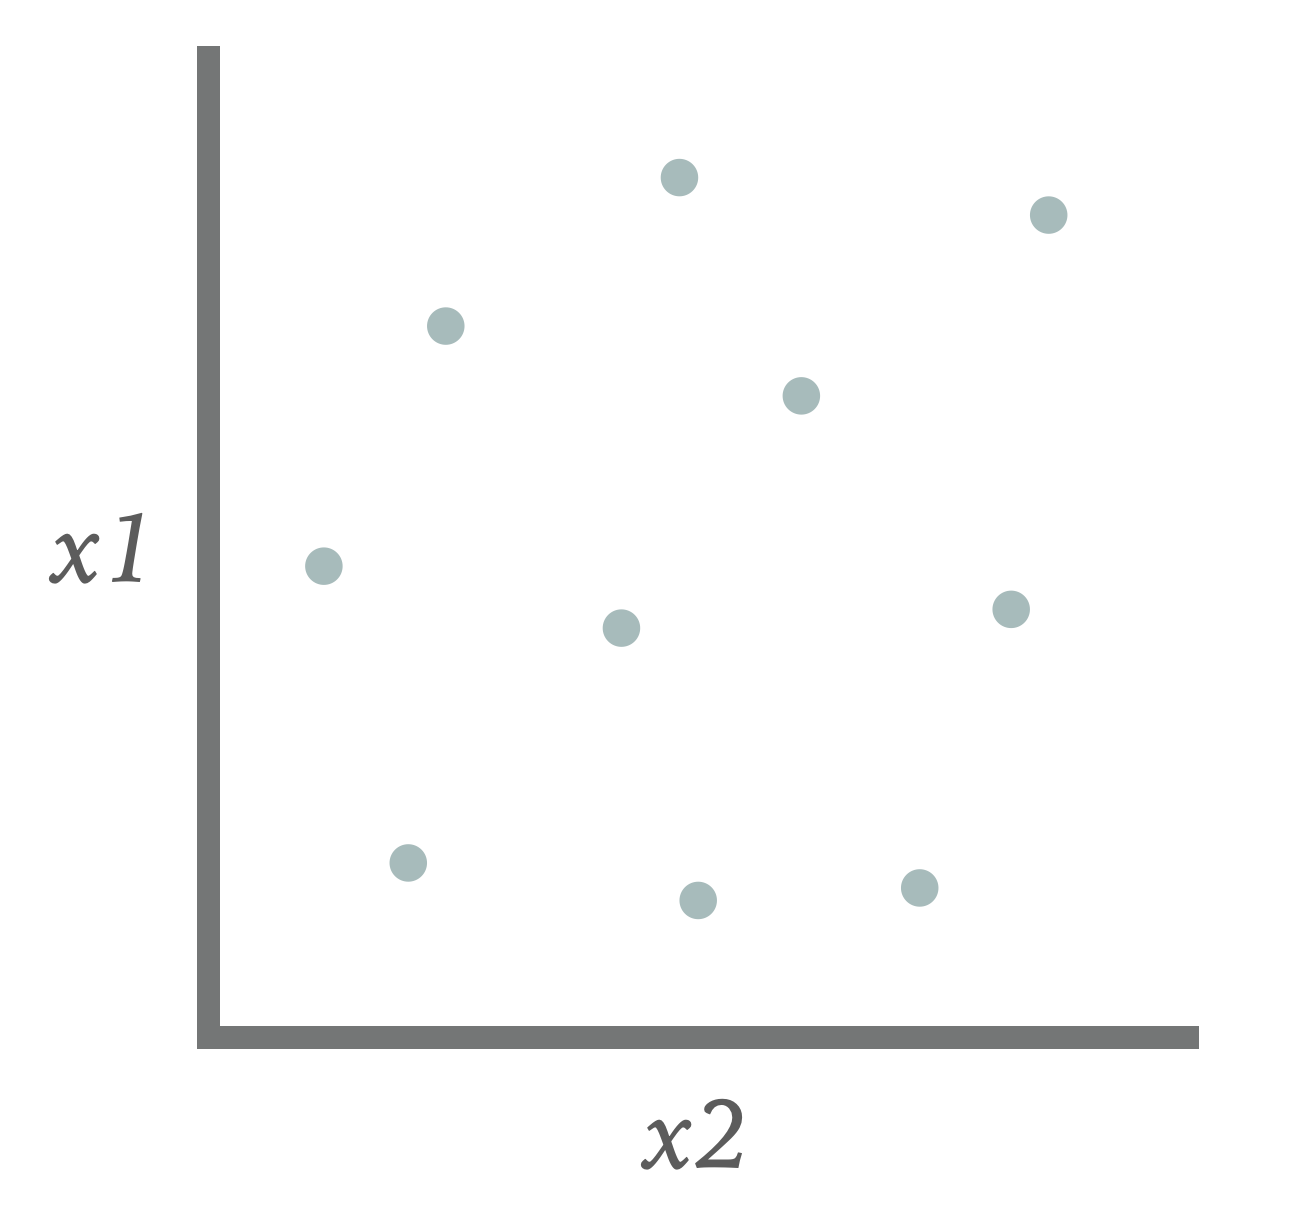
\includegraphics[scale=0.23]{img/initial_big_bang.png}
        \caption{Población tras la fase Big Bang inicial}
\end{figure}

Esta será la primera fase Big Bang, donde la población se habrá expandido uniformemente por todo el espacio.

A continuación ocurre la fase Big Crunch. Actúa como operador de convergencia, donde a partir de todos los individuos de la población se genera una única salida llamada centro de masas. El término masa en este ámbito se refiere a la inversa del valor que toma la función de fitness. Este centro de masas se representa como $\vec{x}^c$ y se calcula con la siguiente fórmula:

\begin{equation}
    \label{eqn:centromasas}
    \vec{x}^c = \frac{\sum^{N}_{i=1}\frac{1}{f^i}\vec{x}^i}{\sum^{N}_{i=1}\frac{1}{f^i}}
\end{equation}

Donde $f^i$ representa el valor fitness del individuo $\vec{x}^i$. Los autores también proponen escoger como centro de masas el individuo con mejor fitness en vez de utilizar esta ecuación. Discutiremos e implementaremos ambas versiones en los siguientes apartados.

\begin{figure}[H]
\centering
    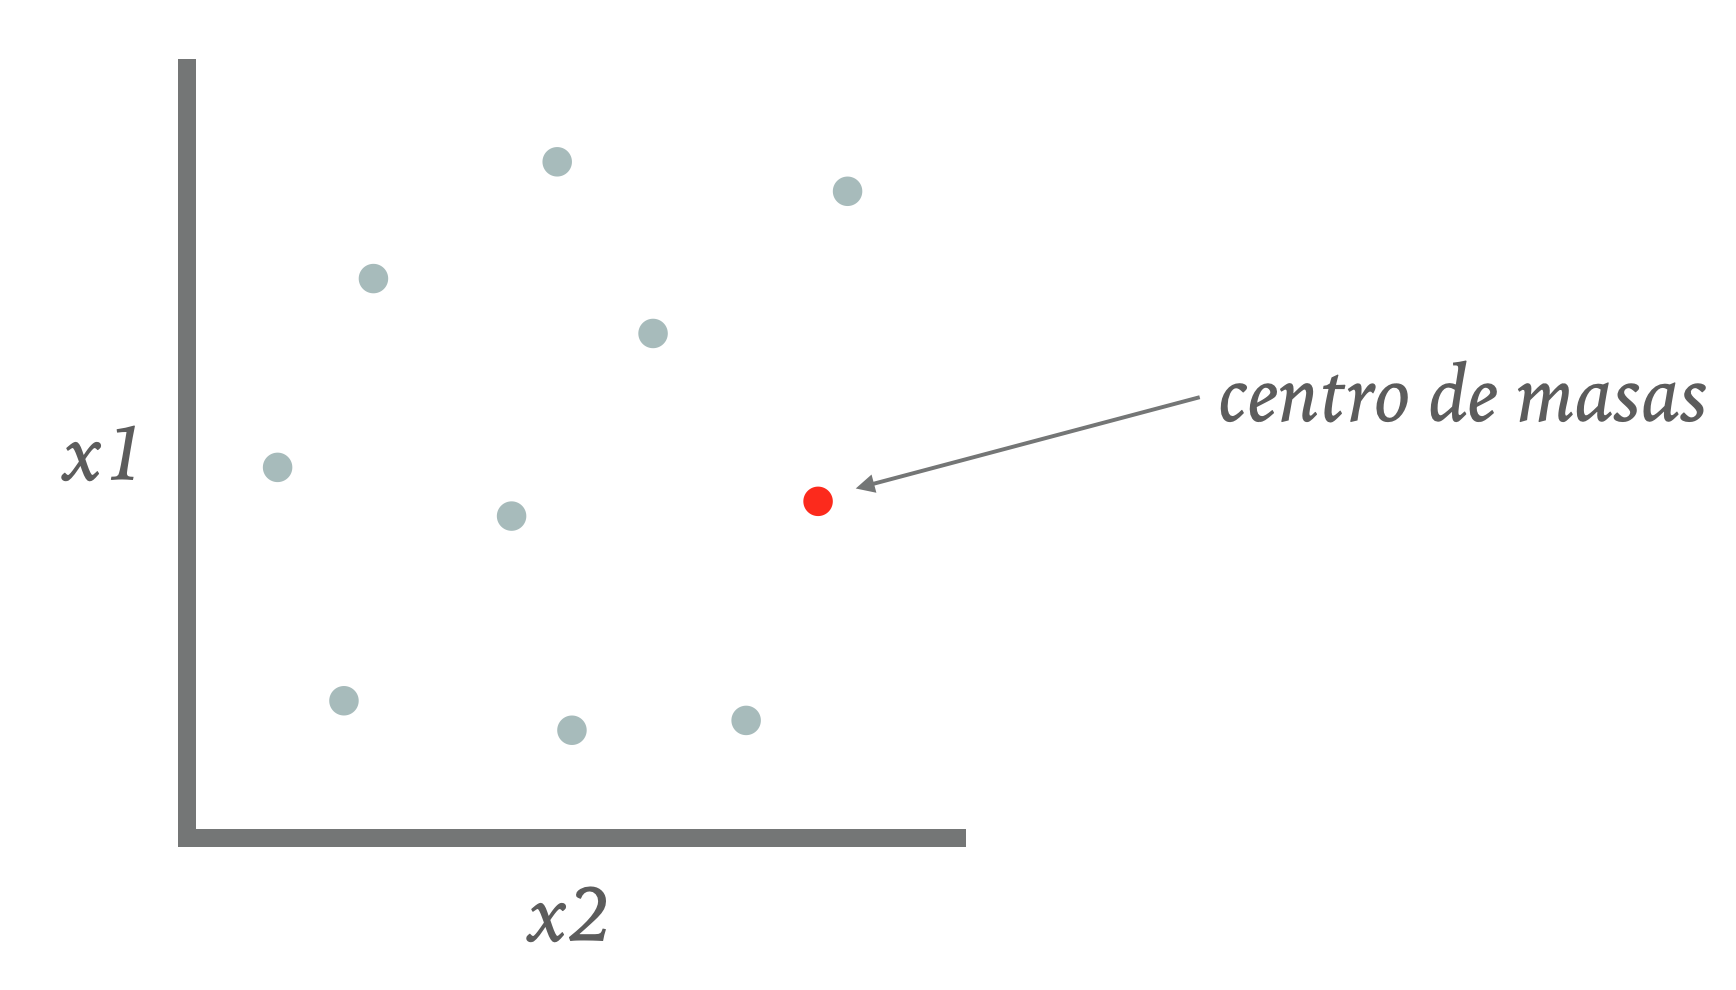
\includegraphics[scale=0.28]{img/big_crunch.png}
    \caption{Elección del centro de masas en la fase Big Crunch}
\end{figure}

Tras la fase Big Crunch, se vuelve a producir otro Big Bang que genera nuevos individuos que reemplazan a la población anterior. Una política de sustitución podría ser la que se utiliza en el Big Bang inicial, generar individuos aleatorios de forma uniforme, pero entonces estaríamos siguiendo una búsqueda aleatoria. Por ello, en la publicación proponen generar los individuos basándose en una distribución normal centrada en el centro de masas. La desviación de los individuos generados irá disminuyendo conforme se lleva a cabo la ejecución, de forma que los puntos se generen cada vez más cerca del centro de masas para que el algoritmo converja. 

\begin{figure}[H]
    \centering
        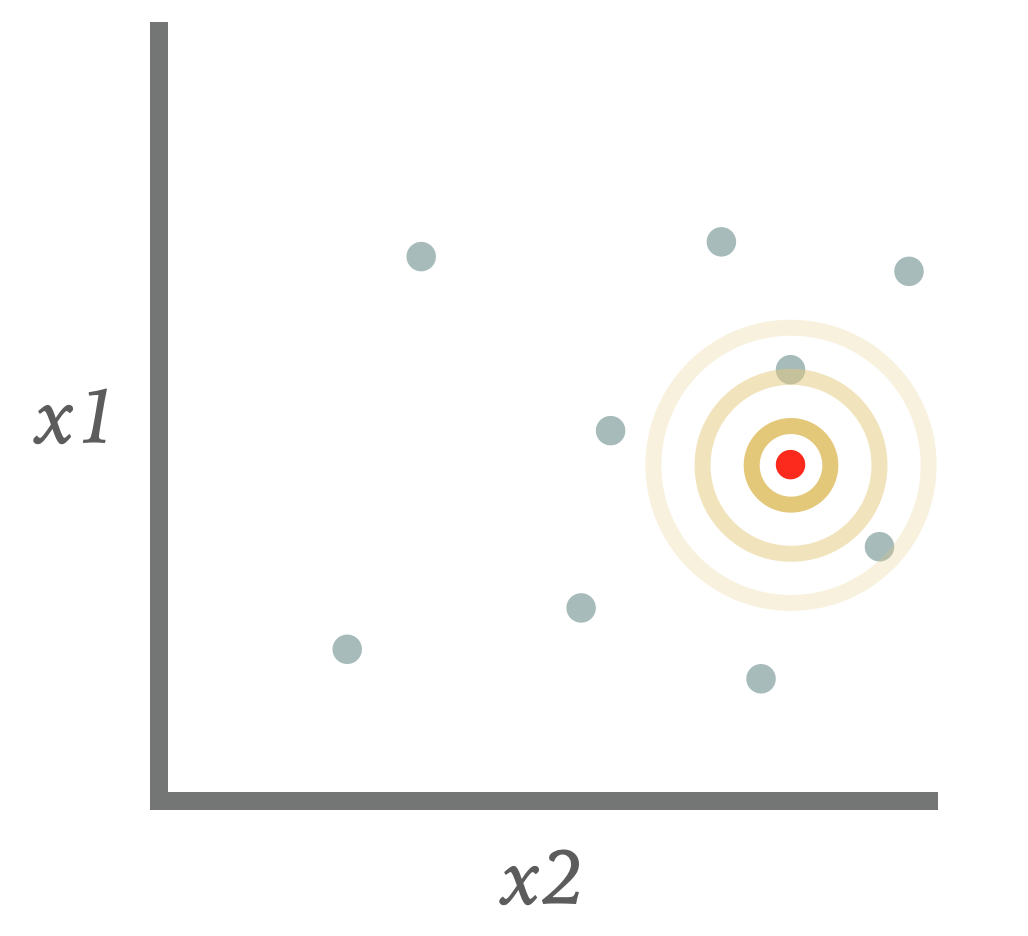
\includegraphics[scale=0.28]{img/big_bang.png}
        \caption{Fase Big Bang genera individuos alrededor de un centro de masas}
    \end{figure}

A nivel de implementación, la generación de nuevos individuos en la fase Big Bang viene dada por la siguiente ecuación, donde $x^c$ es el centro de masas, l el valor máximo que puede tomar un cromosoma, r un valor aleatorio de una distribución normal y k la iteración actual.

\begin{equation}
    \label{eqn:desv}
    x^{new} = x^c + lr/k
\end{equation}

Al realizar este proceso, se debe comprobar que \noindent $x^{new}$ toma valores dentro del dominio permitido (en nuestro caso, [-100, 100]). 

Este proceso Big Bang - Big Crunch se repetirá de forma continuada durante la ejecución del algoritmo, hasta que la condición de parada lo indique. En nuestro caso, el número de evaluaciones de la función objetivo, aunque también podría tomarse el número de iteraciones que se realizan. Con este proceso se espera que la población se reúna en torno a un centro de masas que coincida o sea cercano al óptimo global. Al terminar, se devuelve el mejor individuo de la población. 

\begin{figure}[H]
\centering
    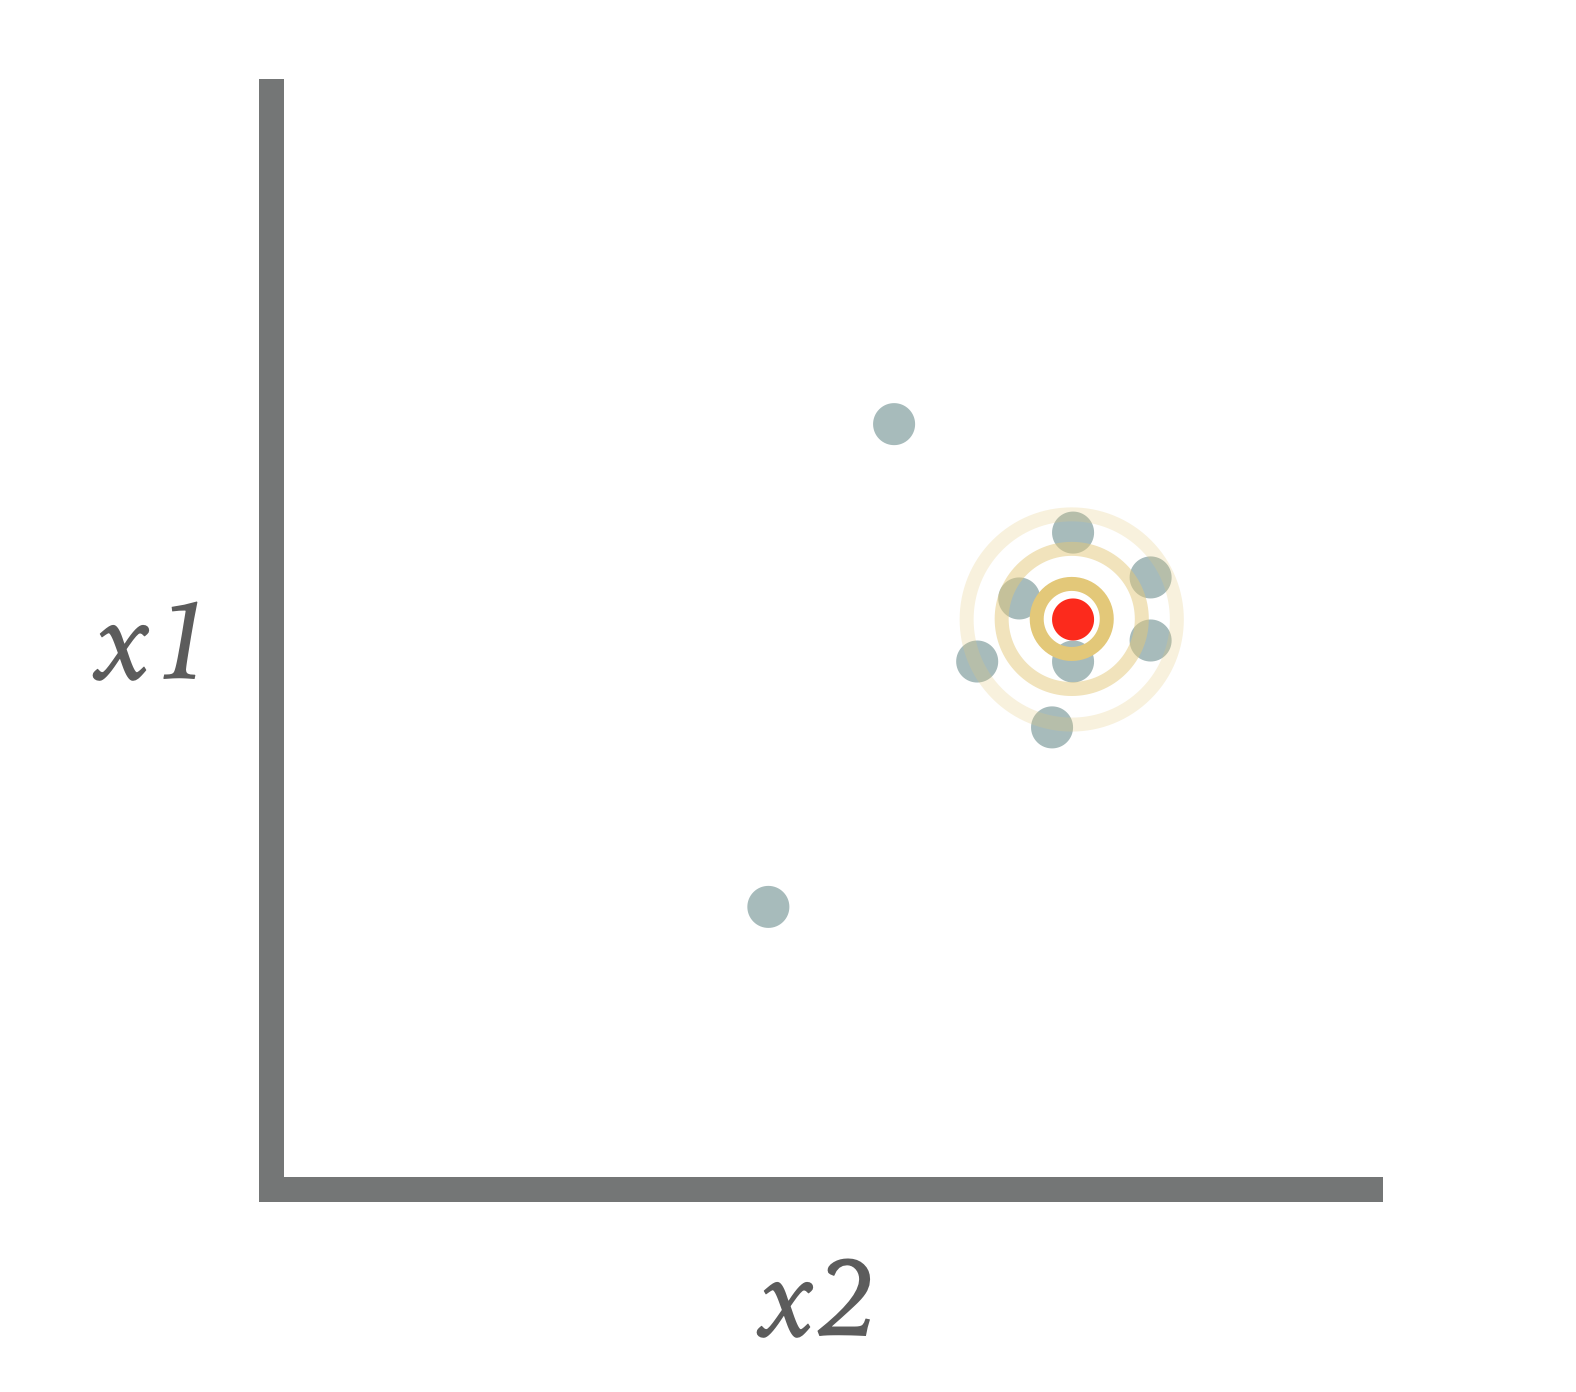
\includegraphics[scale=0.23]{img/end.png}
    \caption{Estado tras la finalización del algoritmo}
\end{figure}

Cada una de las fases del algoritmo trata una de las componentes que son necesarias en este tipo de algoritmos de optimización, la exploración y la explotación. La fase Big Bang coincide con exploración, se generan individuos por todo el espacio de búsqueda, reduciéndose la probabilidad de converger hacia óptimos locales. La fase Big Crunch se encarga de que el algoritmo converja hacia un centro de masas supuestamente cercano a un óptimo. Al inicio de la ejecución, la fase Big Bang puede generar individuos en todo el espacio de búsqueda, pero conforme avanza la generación será de individuos cada vez más cercanos al centro de masas. 

En definitiva, se busca un equilibrio entre exploración y explotación que permita al algoritmo encontrar buenas soluciones.

\part{Pseudocódigo de la Metaheurística}
Explicamos dos versiones, mostrando diferentes formas de implementar el centro de masas. Ambas están contempladas en la publicación original.

Pero antes, mostramos como se inicializa la población en la fase Big Bang inicial:

\begin{algorithm}[H]
\caption{Procedimiento encargado de generar la primera fase Big Bang, generando una población de individuos aleatorios a partir de una distribución uniforme.}
\begin{algorithmic}[1]
\Procedure{InitialBigBang}{population\_size, dim, eval}
  \State population = [ ]
  \For{i = 0 \textbf{to} population\_size - 1}
    \State individual = [ ]
    \For{j = 0 \textbf{to} dim - 1}
      \State individual[j] = RandUniformFloat(-100, 100)
    \EndFor
    \State
    \State individual.fitness = Fitness(individual)
    \State population += {individual}
    \State eval += 1
  \EndFor
  \State
  \State \textbf{return} population, eval
\EndProcedure
\end{algorithmic}
\end{algorithm}

\newpage
\section{Big Bang - Big Crunch (Ecuación \ref{eqn:centromasas})}
En esta primera versión, implementamos el algoritmo con la ecuación \ref{eqn:centromasas} explicada en el apartado anterior. En esta versión, el centro de masas se calcula como una media ponderada del resto de individuos de la población. La ponderación viene dada por la inversa del valor de fitness, de forma que cuanto menor coste tenga el individuo más contribuirá a definir el centro de masas.

\begin{algorithm}[H]
\caption{Big Bang - Big Crunch (Ecuación \ref{eqn:centromasas}): Se implementa el algoritmo Big Bang calculando el centro de masas mediante la ecuación descrita en la publicación.}
\begin{algorithmic}[1]
\Procedure{BigBangBigCrunch\_Equation}{population\_size, dim, MAX\_EVAL}
  \State iter = 1
  \State eval = 0
  \State population, eval = InitialBigBang(population\_size, dim, eval)
  \State
  \While{eval < MAX\_EVAL}
    \State mass\_center, eval = ComputeMassCenter(population, eval, population\_size, dim)
    \State
    \For{i = 0 \textbf{to} population\_size - 1}
      \For{j = 0 \textbf{to} dim - 1}
        \State distance = 100*RandNormalFloat(mean: 0, std: 1)/iter
        \State new\_gen = mass\_center[j] + distance
        \State
        \If{new\_gen > upper\_limit}
          \State new\_gen = upper\_limit
        \EndIf
        \If{new\_gen > lower\_limit}
          \State new\_gen = lower\_limit
        \EndIf
        \State
        \State population[i][j] = new\_gen
      \EndFor
      \State population[i].fitness = Fitness(population[i])
      \State eval += 1
    \EndFor
    \State iter += 1 
  \EndWhile
  \State
  \State SortByFitness(population)
  \State \textbf{return} population[0]
\EndProcedure
\end{algorithmic}
\end{algorithm}

\begin{algorithm}[H]
\caption{Cálculo del centro de masas según la ecuación \ref{eqn:centromasas}.}
\begin{algorithmic}[1]
\Procedure{ComputeMassCenter}{population, eval, population\_size, dim}
  \State mass\_center = [ ] \Comment{Sus elementos se inicializan a 0}
  \State inverted\_fitness = [ ]
  \State sum\_inverted\_fitness = 0
  \State 
  \For{individual $\in$ population}
    \State inverted\_fitness += {1/individual.fitness}
    \State sum\_inverted\_fitness += 1/individual.fitness
  \EndFor
  \State
  \For{i = 0 \textbf{to} population\_size - 1}
    \For{j = 0 \textbf{to} dim - 1}
      \State mass\_center[j] += inverted\_fitness[i] * population[i][j]
    \EndFor
  \EndFor
  \State
  \For{j = 0 \textbf{to} dim - 1}
    \State mass\_center[i] = mass\_center[i]/sum\_inverted\_fitness
  \EndFor
  \State
  \State eval += 1
  \State mass\_center.fitness = Fitness(mass\_center)
  \State \textbf{return} mass\_center, eval
\EndProcedure
\end{algorithmic}
\end{algorithm}

\newpage
\section{Big Bang - Big Crunch (Mejor individuo)}
A continuación, mostramos el pseudocódigo de la versión utilizando el mejor individuo de la población como centro de masas. Es muy similar a la anterior, sólo cambia la parte correspondiente esta elección.
\begin{algorithm}[H]
\caption{Big Bang - Big Crunch (Mejor Individuo): Se implementa el algoritmo Big Bang calculando el centro de masas como el mejor individuo de la población.}
\begin{algorithmic}[1]
\Procedure{BigBangBigCrunch\_BestIndividual}{population\_size, dim, MAX\_EVAL}
  \State iter = 1
  \State eval = 0
  \State population, eval = InitialBigBang(population\_size, dim, eval)
  \State
  \While{eval < MAX\_EVAL}
    \State SortByFitness(population)
    \State mass\_center = population[0]
    \State
    \For{i = 0 \textbf{to} population\_size - 1}
      \For{j = 0 \textbf{to} dim - 1}
        \State distance = 100*RandNormalFloat(mean: 0, std: 1)/iter
        \State new\_gen = mass\_center[j] + distance
        \State
        \If{new\_gen > upper\_limit}
          \State new\_gen = upper\_limit
        \EndIf
        \If{new\_gen > lower\_limit}
          \State new\_gen = lower\_limit
        \EndIf
        \State
        \State population[i][j] = new\_gen
      \EndFor
      \State population[i].fitness = Fitness(population[i])
      \State eval += 1
    \EndFor
    \State iter += 1 
  \EndWhile
  \State
  \State SortByFitness(population)
  \State \textbf{return} population[0]
\EndProcedure
\end{algorithmic}
\end{algorithm}


\part{Experimentación}
En este apartado, tras haber implementado la metaheurística, evaluamos su comportamiento. Para ello utilizamos la suite CEC'2017 que nos permite obtener unos resultados de error estandarizados, para su posterior comparación con otros algoritmos. Las pruebas se realizarán llevando a cabo 10 ejecuciones diferentes y se promediarán los resultados, de forma que se reduzca el efecto de los valores atípicos. 

A continuación, los resultados obtenidos se procesarán en TACOlab \cite{tacolab} donde serán comparados con los de otros algoritmos. TACOlab permite elegir con qué algoritmos se va a realizar la comparación, nosotros elegimos PSO (\textit{Particle Swarm Optimization}, Optimización por enjambre de partículas) y DE (\textit{Differential Evolution}, Evolución diferencial).

PSO es una metaheurística basada en adaptación social que emula el comportamiento de grupos de individuos en la naturaleza, como pueden ser los bancos de peces o una colmena de abejas. Estos seres, de forma individual, tienen un comportamiento simple y no fiable. En cambio al trabajar en grupo, cooperan y se comunican para obtener un resultado de calidad.

Por otro lado, DE es una metaheurística basada en poblaciones. Al igual que otras de esta categoría, parte de una población inicial donde sus individuos se cruzan y mutan simulando la evolución natural.

La experimentación se llevará a cabo con individuos de 4 dimensiones diferentes (10, 30, 50 y 100). Estas dimensiones representan el tamaño de los individuos, el número de genes que los caracterizan. También, se realizarán mediciones en diferentes puntos de la ejecución: cuando se haya completado el 10\% de las evaluaciones, el 50\% y el 100\%.


\section{Metaheurística original}
En esta primera sección evaluamos el rendimiento de la metaheurística original, tal y como viene descrita en el paper. Recordamos que se proponen dos formas de calcular el centro de masas, utilizando la ecuación \ref{eqn:centromasas} o tomando el mejor individuo. Vamos a evaluar los resultados de ambas.

\subsection{Versión 1: Centro de masas calculado como en la ecuación \ref{eqn:centromasas}}

\subsubsection*{10\% de las evaluaciones}

\begin{table}[H]
    \begin{minipage}{.5\linewidth}
      \caption{Dimensión 10}
      \centering
      \begin{tabular}{llll}
        \toprule
        {} &     BB-BC &        DE &       PSO \\
        \midrule
        F01  &  2.39e+09 &  3.14e+07 &  8.30e+08 \\
        F02  &  9.27e+06 &  6.05e+03 &  1.00e+00 \\
        F03  &  4.45e+04 &  1.39e+03 &  1.28e+04 \\
        F04  &  6.86e+01 &  9.80e+00 &  1.16e+02 \\
        F05  &  1.46e+02 &  1.17e+02 &  7.09e+01 \\
        F06  &  8.31e+01 &  5.06e+01 &  2.59e+01 \\
        F07  &  1.36e+02 &  7.78e+01 &  8.90e+01 \\
        F08  &  6.43e+01 &  3.08e+01 &  5.69e+01 \\
        F09  &  1.00e+02 &  8.09e+02 &  2.95e+02 \\
        F10  &  2.13e+03 &  1.37e+03 &  1.59e+03 \\
        F11  &  7.93e+02 &  2.45e+01 &  1.16e+02 \\
        F12  &  2.76e+05 &  4.77e+04 &  2.63e+07 \\
        F13  &  8.92e+03 &  4.17e+02 &  1.48e+05 \\
        F14  &  1.62e+03 &  3.50e+01 &  5.51e+02 \\
        F15  &  1.40e+04 &  1.50e+01 &  8.78e+03 \\
        F16  &  3.87e+02 &  4.62e+02 &  3.42e+02 \\
        F17  &  1.63e+02 &  5.31e+01 &  1.31e+02 \\
        F18  &  7.93e+03 &  1.13e+02 &  2.36e+05 \\
        F19  &  2.67e+04 &  9.46e+00 &  2.36e+04 \\
        F20  &  2.44e+02 &  3.91e+02 &  1.78e+02 \\
        F21  &  2.75e+02 &  2.09e+02 &  1.89e+02 \\
        F22  &  6.50e+02 &  1.14e+02 &  1.61e+02 \\
        F23  &  4.85e+02 &  8.28e+02 &  3.58e+02 \\
        F24  &  4.97e+02 &  1.11e+02 &  2.66e+02 \\
        F25  &  1.09e+03 &  4.12e+02 &  4.84e+02 \\
        F26  &  2.21e+03 &  3.28e+02 &  6.01e+02 \\
        F27  &  6.13e+02 &  4.01e+02 &  4.49e+02 \\
        F28  &  9.46e+02 &  4.10e+02 &  7.36e+02 \\
        F29  &  5.18e+02 &  3.25e+02 &  4.30e+02 \\
        F30  &  1.32e+07 &  1.23e+05 &  3.77e+06 \\
        Best &         1 &        22 &         7 \\
        \bottomrule
        \end{tabular}
        
    \end{minipage}%
    \begin{minipage}{.5\linewidth}
      \centering
        \caption{Dimensión 30}
        \begin{tabular}{llll}
            \toprule
            {} &     BB-BC &        DE &       PSO \\
            \midrule
            F01  &  3.67e+10 &  5.81e+09 &  1.39e+10 \\
            F02  &  4.51e+25 &  3.90e+32 &  1.00e+00 \\
            F03  &  2.85e+05 &  5.87e+04 &  1.18e+05 \\
            F04  &  5.57e+03 &  7.58e+02 &  3.36e+03 \\
            F05  &  4.49e+02 &  3.51e+02 &  3.23e+02 \\
            F06  &  1.04e+02 &  7.81e+01 &  6.37e+01 \\
            F07  &  5.98e+02 &  3.29e+02 &  5.15e+02 \\
            F08  &  3.94e+02 &  2.82e+02 &  2.89e+02 \\
            F09  &  3.94e+03 &  9.91e+03 &  7.07e+03 \\
            F10  &  7.89e+03 &  5.59e+03 &  7.89e+03 \\
            F11  &  1.65e+04 &  5.10e+02 &  3.21e+03 \\
            F12  &  6.99e+09 &  3.39e+08 &  1.86e+09 \\
            F13  &  3.59e+04 &  2.22e+07 &  1.02e+09 \\
            F14  &  3.04e+06 &  1.32e+03 &  1.01e+06 \\
            F15  &  1.34e+04 &  5.93e+04 &  1.20e+07 \\
            F16  &  3.59e+03 &  2.01e+03 &  2.51e+03 \\
            F17  &  1.13e+03 &  8.71e+02 &  9.47e+02 \\
            F18  &  3.53e+06 &  2.43e+05 &  1.34e+07 \\
            F19  &  4.55e+05 &  4.29e+05 &  2.15e+07 \\
            F20  &  1.42e+03 &  5.70e+02 &  9.21e+02 \\
            F21  &  6.79e+02 &  4.05e+02 &  5.19e+02 \\
            F22  &  7.79e+03 &  9.19e+02 &  2.33e+03 \\
            F23  &  1.44e+03 &  6.29e+02 &  7.58e+02 \\
            F24  &  1.89e+03 &  6.87e+02 &  8.11e+02 \\
            F25  &  1.68e+03 &  6.30e+02 &  1.16e+03 \\
            F26  &  7.76e+03 &  2.09e+03 &  4.60e+03 \\
            F27  &  2.33e+03 &  6.23e+02 &  1.08e+03 \\
            F28  &  4.39e+03 &  8.20e+02 &  1.84e+03 \\
            F29  &  4.09e+03 &  1.61e+03 &  2.24e+03 \\
            F30  &  2.24e+07 &  3.83e+06 &  6.12e+07 \\
            Best &         3 &        24 &         3 \\
            \bottomrule
            \end{tabular}
            
    \end{minipage} 
\end{table}

\begin{table}[H]
    \begin{minipage}{.5\linewidth}
      \caption{Dimensión 50}
      \centering
      \begin{tabular}{llll}
        \toprule
        {} &     BB-BC &        DE &       PSO \\
        \midrule
        F01  &  7.53e+10 &  2.53e+10 &  4.33e+10 \\
        F02  &  2.36e+37 &  2.37e+62 &  1.00e+00 \\
        F03  &  5.80e+05 &  1.41e+05 &  2.41e+05 \\
        F04  &  1.97e+04 &  3.86e+03 &  9.35e+03 \\
        F05  &  6.81e+02 &  5.86e+02 &  5.97e+02 \\
        F06  &  1.10e+02 &  9.23e+01 &  7.93e+01 \\
        F07  &  1.42e+03 &  6.94e+02 &  1.08e+03 \\
        F08  &  7.21e+02 &  6.14e+02 &  5.57e+02 \\
        F09  &  1.81e+04 &  3.54e+04 &  3.00e+04 \\
        F10  &  1.41e+04 &  1.22e+04 &  1.42e+04 \\
        F11  &  5.06e+04 &  2.91e+03 &  1.04e+04 \\
        F12  &  4.97e+10 &  5.93e+09 &  1.55e+10 \\
        F13  &  1.26e+10 &  8.60e+08 &  4.03e+09 \\
        F14  &  3.51e+05 &  4.35e+05 &  9.94e+06 \\
        F15  &  2.00e+08 &  1.84e+07 &  2.00e+08 \\
        F16  &  4.89e+03 &  3.92e+03 &  4.10e+03 \\
        F17  &  2.33e+03 &  2.39e+03 &  2.53e+03 \\
        F18  &  6.24e+07 &  3.77e+06 &  3.86e+07 \\
        F19  &  2.17e+05 &  1.82e+07 &  1.65e+08 \\
        F20  &  2.01e+03 &  1.33e+03 &  2.29e+03 \\
        F21  &  1.09e+03 &  7.45e+02 &  8.49e+02 \\
        F22  &  1.64e+04 &  1.33e+04 &  1.42e+04 \\
        F23  &  2.58e+03 &  1.10e+03 &  1.27e+03 \\
        F24  &  2.50e+03 &  1.10e+03 &  1.43e+03 \\
        F25  &  9.63e+03 &  2.47e+03 &  5.77e+03 \\
        F26  &  1.44e+04 &  4.38e+03 &  9.44e+03 \\
        F27  &  5.19e+03 &  1.29e+03 &  2.32e+03 \\
        F28  &  8.42e+03 &  2.70e+03 &  4.72e+03 \\
        F29  &  5.83e+03 &  3.61e+03 &  5.58e+03 \\
        F30  &  5.20e+08 &  2.03e+08 &  8.37e+08 \\
        Best &         4 &        23 &         3 \\
        \bottomrule
        \end{tabular}
        
    \end{minipage}%
    \begin{minipage}{.5\linewidth}
      \centering
      \caption{Dimensión 100}
      \begin{tabular}{llll}
        \toprule
        {} &      BB-BC &         DE &       PSO \\
        \midrule
        F01  &   2.61e+11 &   1.05e+11 &  1.64e+11 \\
        F02  &  7.39e+124 &  2.11e+145 &  1.00e+00 \\
        F03  &   7.52e+05 &   3.20e+05 &  5.12e+05 \\
        F04  &   5.82e+04 &   2.30e+04 &  3.70e+04 \\
        F05  &   1.50e+03 &   1.39e+03 &  1.48e+03 \\
        F06  &   1.11e+02 &   1.03e+02 &  9.71e+01 \\
        F07  &   3.20e+03 &   1.94e+03 &  2.94e+03 \\
        F08  &   1.78e+03 &   1.31e+03 &  1.50e+03 \\
        F09  &   3.14e+04 &   7.68e+04 &  8.35e+04 \\
        F10  &   3.02e+04 &   2.73e+04 &  3.12e+04 \\
        F11  &   2.08e+05 &   1.37e+05 &  1.82e+05 \\
        F12  &   1.73e+11 &   4.40e+10 &  6.31e+10 \\
        F13  &   3.19e+10 &   5.42e+09 &  9.41e+09 \\
        F14  &   1.09e+07 &   7.47e+06 &  4.61e+07 \\
        F15  &   1.30e+10 &   1.14e+09 &  2.27e+09 \\
        F16  &   1.97e+04 &   1.04e+04 &  1.21e+04 \\
        F17  &   5.74e+03 &   8.08e+03 &  1.36e+04 \\
        F18  &   1.32e+07 &   1.43e+07 &  1.01e+08 \\
        F19  &   1.48e+10 &   1.22e+09 &  2.58e+09 \\
        F20  &   6.15e+03 &   5.03e+03 &  5.86e+03 \\
        F21  &   3.08e+03 &   1.86e+03 &  2.00e+03 \\
        F22  &   3.34e+04 &   2.98e+04 &  3.26e+04 \\
        F23  &   4.89e+03 &   2.34e+03 &  2.72e+03 \\
        F24  &   9.32e+03 &   3.50e+03 &  4.11e+03 \\
        F25  &   1.95e+04 &   1.02e+04 &  1.42e+04 \\
        F26  &   4.89e+04 &   2.16e+04 &  2.88e+04 \\
        F27  &   1.28e+04 &   3.08e+03 &  4.28e+03 \\
        F28  &   2.60e+04 &   1.43e+04 &  1.67e+04 \\
        F29  &   1.30e+04 &   1.13e+04 &  1.49e+04 \\
        F30  &   3.10e+10 &   2.13e+09 &  6.92e+09 \\
        Best &          3 &         25 &         2 \\
        \bottomrule
        \end{tabular}
        
    \end{minipage} 
\end{table}


\subsubsection*{50\% de las evaluaciones}

\begin{table}[H]
    \begin{minipage}{.5\linewidth}
      \caption{Dimensión 10}
      \centering
      \begin{tabular}{llll}
        \toprule
        {} &     BB-BC &        DE &       PSO \\
        \midrule
        F01  &  2.39e+09 &  2.00e-05 &  1.85e+08 \\
        F02  &  8.16e+06 &  0.00e+00 &  1.00e+00 \\
        F03  &  4.45e+04 &  2.81e-08 &  3.46e+03 \\
        F04  &  6.86e+01 &  2.36e-01 &  6.36e+01 \\
        F05  &  1.46e+02 &  1.15e+02 &  4.73e+01 \\
        F06  &  8.31e+01 &  3.47e+01 &  1.36e+01 \\
        F07  &  1.36e+02 &  4.38e+01 &  5.70e+01 \\
        F08  &  6.43e+01 &  2.98e+01 &  2.97e+01 \\
        F09  &  9.12e+01 &  2.09e+02 &  8.36e+01 \\
        F10  &  2.13e+03 &  5.31e+02 &  1.32e+03 \\
        F11  &  7.93e+02 &  5.90e+00 &  5.04e+01 \\
        F12  &  2.66e+05 &  7.66e+01 &  4.64e+06 \\
        F13  &  8.38e+03 &  1.11e+01 &  1.23e+04 \\
        F14  &  1.60e+03 &  1.54e+01 &  1.64e+02 \\
        F15  &  1.40e+04 &  4.37e-01 &  3.23e+03 \\
        F16  &  3.87e+02 &  4.56e+02 &  1.85e+02 \\
        F17  &  1.63e+02 &  3.12e+01 &  7.63e+01 \\
        F18  &  7.93e+03 &  1.67e-01 &  2.65e+04 \\
        F19  &  2.67e+04 &  4.60e-01 &  5.86e+03 \\
        F20  &  2.39e+02 &  3.84e+02 &  1.10e+02 \\
        F21  &  2.75e+02 &  1.92e+02 &  1.42e+02 \\
        F22  &  6.50e+02 &  1.02e+02 &  1.03e+02 \\
        F23  &  4.85e+02 &  8.12e+02 &  3.37e+02 \\
        F24  &  4.97e+02 &  1.00e+02 &  2.04e+02 \\
        F25  &  1.09e+03 &  4.04e+02 &  4.54e+02 \\
        F26  &  2.21e+03 &  2.71e+02 &  4.17e+02 \\
        F27  &  6.13e+02 &  3.90e+02 &  4.20e+02 \\
        F28  &  9.46e+02 &  3.52e+02 &  5.24e+02 \\
        F29  &  5.18e+02 &  2.51e+02 &  3.51e+02 \\
        F30  &  1.32e+07 &  8.05e+04 &  1.48e+06 \\
        Best &         0 &        22 &         8 \\
        \bottomrule
        \end{tabular}
        
        
    \end{minipage}%
    \begin{minipage}{.5\linewidth}
      \centering
        \caption{Dimensión 30}
        \begin{tabular}{llll}
            \toprule
            {} &     BB-BC &        DE &       PSO \\
            \midrule
            F01  &  3.67e+10 &  1.79e+07 &  7.70e+09 \\
            F02  &  3.62e+25 &  5.44e+23 &  1.00e+00 \\
            F03  &  2.85e+05 &  1.37e+04 &  7.12e+04 \\
            F04  &  5.57e+03 &  9.42e+01 &  1.66e+03 \\
            F05  &  4.49e+02 &  2.20e+02 &  2.60e+02 \\
            F06  &  1.04e+02 &  2.14e+01 &  4.67e+01 \\
            F07  &  5.98e+02 &  2.52e+02 &  4.10e+02 \\
            F08  &  3.94e+02 &  2.09e+02 &  2.16e+02 \\
            F09  &  3.37e+03 &  2.78e+03 &  4.10e+03 \\
            F10  &  7.89e+03 &  4.42e+03 &  7.43e+03 \\
            F11  &  1.65e+04 &  1.12e+02 &  1.56e+03 \\
            F12  &  6.99e+09 &  5.64e+06 &  6.94e+08 \\
            F13  &  3.10e+04 &  1.51e+03 &  2.36e+08 \\
            F14  &  3.04e+06 &  8.11e+01 &  4.77e+05 \\
            F15  &  1.28e+04 &  1.14e+02 &  1.26e+06 \\
            F16  &  3.59e+03 &  1.51e+03 &  1.86e+03 \\
            F17  &  1.13e+03 &  5.82e+02 &  5.51e+02 \\
            F18  &  3.53e+06 &  3.29e+02 &  4.17e+06 \\
            F19  &  4.33e+05 &  4.63e+01 &  2.33e+06 \\
            F20  &  1.42e+03 &  3.11e+02 &  6.19e+02 \\
            F21  &  6.79e+02 &  3.50e+02 &  4.49e+02 \\
            F22  &  7.79e+03 &  1.18e+02 &  1.35e+03 \\
            F23  &  1.44e+03 &  5.52e+02 &  6.91e+02 \\
            F24  &  1.89e+03 &  6.21e+02 &  7.47e+02 \\
            F25  &  1.68e+03 &  3.90e+02 &  7.75e+02 \\
            F26  &  7.76e+03 &  4.90e+02 &  3.73e+03 \\
            F27  &  2.33e+03 &  5.15e+02 &  8.85e+02 \\
            F28  &  4.39e+03 &  4.37e+02 &  1.29e+03 \\
            F29  &  4.09e+03 &  1.17e+03 &  1.61e+03 \\
            F30  &  2.22e+07 &  1.57e+04 &  2.02e+07 \\
            Best &         0 &        28 &         2 \\
            \bottomrule
            \end{tabular}
            
    \end{minipage} 
\end{table}

\begin{table}[H]
    \begin{minipage}{.5\linewidth}
      \caption{Dimensión 50}
      \centering
      \begin{tabular}{llll}
        \toprule
        {} &     BB-BC &        DE &       PSO \\
        \midrule
        F01  &  7.53e+10 &  2.17e+09 &  2.77e+10 \\
        F02  &  1.19e+37 &  4.83e+55 &  1.00e+00 \\
        F03  &  5.80e+05 &  9.97e+04 &  1.56e+05 \\
        F04  &  1.97e+04 &  4.73e+02 &  5.62e+03 \\
        F05  &  6.81e+02 &  4.20e+02 &  5.04e+02 \\
        F06  &  1.10e+02 &  3.05e+01 &  6.43e+01 \\
        F07  &  1.42e+03 &  5.14e+02 &  9.02e+02 \\
        F08  &  7.21e+02 &  4.28e+02 &  4.62e+02 \\
        F09  &  1.19e+04 &  2.76e+04 &  2.12e+04 \\
        F10  &  1.41e+04 &  1.15e+04 &  1.37e+04 \\
        F11  &  5.06e+04 &  3.58e+02 &  4.51e+03 \\
        F12  &  4.97e+10 &  4.92e+08 &  8.92e+09 \\
        F13  &  1.26e+10 &  1.17e+06 &  1.63e+09 \\
        F14  &  3.36e+05 &  2.68e+02 &  2.88e+06 \\
        F15  &  1.42e+08 &  4.14e+03 &  2.74e+07 \\
        F16  &  4.89e+03 &  3.28e+03 &  3.13e+03 \\
        F17  &  2.33e+03 &  1.99e+03 &  1.82e+03 \\
        F18  &  6.24e+07 &  2.09e+05 &  1.80e+07 \\
        F19  &  2.17e+05 &  3.56e+03 &  3.43e+07 \\
        F20  &  2.01e+03 &  9.67e+02 &  1.58e+03 \\
        F21  &  1.09e+03 &  6.43e+02 &  7.51e+02 \\
        F22  &  1.64e+04 &  6.64e+02 &  1.33e+04 \\
        F23  &  2.58e+03 &  8.76e+02 &  1.16e+03 \\
        F24  &  2.50e+03 &  9.11e+02 &  1.27e+03 \\
        F25  &  9.63e+03 &  7.40e+02 &  3.76e+03 \\
        F26  &  1.44e+04 &  1.48e+03 &  8.46e+03 \\
        F27  &  5.19e+03 &  6.95e+02 &  1.91e+03 \\
        F28  &  8.42e+03 &  6.62e+02 &  3.88e+03 \\
        F29  &  5.83e+03 &  2.48e+03 &  4.27e+03 \\
        F30  &  4.97e+08 &  8.86e+06 &  4.57e+08 \\
        Best &         1 &        26 &         3 \\
        \bottomrule
        \end{tabular}
        
    \end{minipage}%
    \begin{minipage}{.5\linewidth}
      \centering
      \caption{Dimensión 100}
      \begin{tabular}{llll}
        \toprule
        {} &      BB-BC &         DE &       PSO \\
        \midrule
        F01  &   2.61e+11 &   3.27e+10 &  1.33e+11 \\
        F02  &  6.04e+124 &  6.15e+138 &  1.00e+00 \\
        F03  &   7.52e+05 &   2.69e+05 &  3.67e+05 \\
        F04  &   5.82e+04 &   3.95e+03 &  2.77e+04 \\
        F05  &   1.50e+03 &   1.04e+03 &  1.32e+03 \\
        F06  &   1.11e+02 &   5.46e+01 &  8.43e+01 \\
        F07  &   3.20e+03 &   1.39e+03 &  2.54e+03 \\
        F08  &   1.78e+03 &   1.05e+03 &  1.35e+03 \\
        F09  &   2.70e+04 &   7.18e+04 &  6.80e+04 \\
        F10  &   3.02e+04 &   2.63e+04 &  3.06e+04 \\
        F11  &   2.08e+05 &   5.86e+04 &  8.64e+04 \\
        F12  &   1.73e+11 &   1.05e+10 &  4.69e+10 \\
        F13  &   3.19e+10 &   2.98e+08 &  6.05e+09 \\
        F14  &   1.09e+07 &   1.17e+06 &  2.72e+07 \\
        F15  &   1.30e+10 &   1.15e+07 &  6.84e+08 \\
        F16  &   1.97e+04 &   8.95e+03 &  9.97e+03 \\
        F17  &   5.63e+03 &   5.87e+03 &  7.20e+03 \\
        F18  &   1.30e+07 &   6.53e+06 &  3.11e+07 \\
        F19  &   1.48e+10 &   3.44e+07 &  1.19e+09 \\
        F20  &   6.15e+03 &   4.26e+03 &  5.45e+03 \\
        F21  &   3.08e+03 &   1.35e+03 &  1.81e+03 \\
        F22  &   3.34e+04 &   7.25e+03 &  3.19e+04 \\
        F23  &   4.89e+03 &   1.65e+03 &  2.48e+03 \\
        F24  &   9.32e+03 &   2.04e+03 &  3.65e+03 \\
        F25  &   1.95e+04 &   4.07e+03 &  1.10e+04 \\
        F26  &   4.89e+04 &   1.47e+04 &  2.65e+04 \\
        F27  &   1.28e+04 &   1.41e+03 &  3.57e+03 \\
        F28  &   2.60e+04 &   3.67e+03 &  1.41e+04 \\
        F29  &   1.30e+04 &   7.58e+03 &  1.20e+04 \\
        F30  &   3.10e+10 &   5.22e+07 &  4.51e+09 \\
        Best &          2 &         27 &         1 \\
        \bottomrule
        \end{tabular}
        
    \end{minipage} 
\end{table}


\subsubsection*{100\% de las evaluaciones}

\begin{table}[H]
    \begin{minipage}{.5\linewidth}
      \caption{Dimensión 10}
      \centering
      \begin{tabular}{llll}
        \toprule
        {} &     BB-BC &        DE &       PSO \\
        \midrule
        F01  &  2.39e+09 &  0.00e+00 &  5.26e+07 \\
        F02  &  7.58e+06 &  0.00e+00 &  1.00e+00 \\
        F03  &  4.45e+04 &  0.00e+00 &  1.99e+03 \\
        F04  &  6.86e+01 &  1.11e-04 &  4.68e+01 \\
        F05  &  1.46e+02 &  1.15e+02 &  3.21e+01 \\
        F06  &  8.31e+01 &  3.46e+01 &  1.00e+01 \\
        F07  &  1.36e+02 &  3.85e+01 &  4.28e+01 \\
        F08  &  6.43e+01 &  2.98e+01 &  2.20e+01 \\
        F09  &  9.12e+01 &  1.94e+02 &  5.69e+01 \\
        F10  &  2.13e+03 &  3.60e+02 &  1.08e+03 \\
        F11  &  7.93e+02 &  1.94e-02 &  3.84e+01 \\
        F12  &  2.61e+05 &  4.93e+00 &  2.52e+06 \\
        F13  &  8.32e+03 &  5.99e+00 &  8.41e+03 \\
        F14  &  1.60e+03 &  5.24e-02 &  9.99e+01 \\
        F15  &  1.40e+04 &  6.06e-02 &  2.07e+03 \\
        F16  &  3.87e+02 &  4.56e+02 &  1.41e+02 \\
        F17  &  1.63e+02 &  2.35e+01 &  6.50e+01 \\
        F18  &  7.93e+03 &  3.63e-02 &  1.48e+04 \\
        F19  &  2.67e+04 &  5.19e-03 &  3.22e+03 \\
        F20  &  2.39e+02 &  3.84e+02 &  8.44e+01 \\
        F21  &  2.75e+02 &  1.89e+02 &  1.32e+02 \\
        F22  &  6.50e+02 &  1.00e+02 &  7.74e+01 \\
        F23  &  4.85e+02 &  8.10e+02 &  3.30e+02 \\
        F24  &  4.97e+02 &  1.00e+02 &  1.81e+02 \\
        F25  &  1.09e+03 &  4.04e+02 &  4.48e+02 \\
        F26  &  2.21e+03 &  2.71e+02 &  3.73e+02 \\
        F27  &  6.13e+02 &  3.90e+02 &  4.13e+02 \\
        F28  &  9.46e+02 &  3.52e+02 &  4.70e+02 \\
        F29  &  5.18e+02 &  2.38e+02 &  3.19e+02 \\
        F30  &  1.32e+07 &  8.05e+04 &  6.35e+05 \\
        Best &         0 &        21 &         9 \\
        \bottomrule
        \end{tabular}
        
    \end{minipage}%
    \begin{minipage}{.5\linewidth}
      \centering
        \caption{Dimensión 30}
        \begin{tabular}{llll}
            \toprule
            {} &     BB-BC &        DE &       PSO \\
            \midrule
            F01  &  3.67e+10 &  4.91e+04 &  4.18e+09 \\
            F02  &  3.47e+25 &  1.31e+19 &  1.00e+00 \\
            F03  &  2.85e+05 &  3.48e+03 &  5.45e+04 \\
            F04  &  5.57e+03 &  8.43e+01 &  1.18e+03 \\
            F05  &  4.49e+02 &  2.01e+02 &  2.17e+02 \\
            F06  &  1.04e+02 &  6.32e+00 &  3.69e+01 \\
            F07  &  5.98e+02 &  2.33e+02 &  3.60e+02 \\
            F08  &  3.94e+02 &  1.89e+02 &  1.75e+02 \\
            F09  &  3.37e+03 &  6.53e+01 &  2.84e+03 \\
            F10  &  7.89e+03 &  3.76e+03 &  6.94e+03 \\
            F11  &  1.65e+04 &  7.96e+01 &  1.21e+03 \\
            F12  &  6.99e+09 &  3.26e+05 &  3.59e+08 \\
            F13  &  3.10e+04 &  1.54e+02 &  4.51e+07 \\
            F14  &  3.04e+06 &  7.10e+01 &  3.06e+05 \\
            F15  &  1.27e+04 &  6.26e+01 &  2.74e+05 \\
            F16  &  3.59e+03 &  1.32e+03 &  1.57e+03 \\
            F17  &  1.13e+03 &  4.81e+02 &  4.73e+02 \\
            F18  &  3.51e+06 &  6.12e+01 &  2.17e+06 \\
            F19  &  4.33e+05 &  3.57e+01 &  1.26e+06 \\
            F20  &  1.42e+03 &  2.75e+02 &  4.62e+02 \\
            F21  &  6.79e+02 &  3.25e+02 &  4.11e+02 \\
            F22  &  7.79e+03 &  1.00e+02 &  1.03e+03 \\
            F23  &  1.44e+03 &  5.35e+02 &  6.40e+02 \\
            F24  &  1.89e+03 &  6.06e+02 &  7.10e+02 \\
            F25  &  1.68e+03 &  3.87e+02 &  6.86e+02 \\
            F26  &  7.76e+03 &  4.04e+02 &  3.37e+03 \\
            F27  &  2.33e+03 &  4.93e+02 &  8.07e+02 \\
            F28  &  4.39e+03 &  3.94e+02 &  1.11e+03 \\
            F29  &  4.09e+03 &  1.03e+03 &  1.41e+03 \\
            F30  &  2.22e+07 &  3.66e+03 &  1.36e+07 \\
            Best &         0 &        27 &         3 \\
            \bottomrule
            \end{tabular}
            
    \end{minipage} 
\end{table}

\begin{table}[H]
    \begin{minipage}{.5\linewidth}
      \caption{Dimensión 50}
      \centering
      \begin{tabular}{llll}
        \toprule
        {} &     BB-BC &        DE &       PSO \\
        \midrule
        F01  &  7.53e+10 &  2.04e+08 &  1.82e+10 \\
        F02  &  1.19e+37 &  5.16e+52 &  1.00e+00 \\
        F03  &  5.80e+05 &  7.60e+04 &  1.01e+05 \\
        F04  &  1.97e+04 &  2.32e+02 &  4.09e+03 \\
        F05  &  6.81e+02 &  3.98e+02 &  4.33e+02 \\
        F06  &  1.10e+02 &  1.18e+01 &  5.45e+01 \\
        F07  &  1.42e+03 &  4.78e+02 &  8.20e+02 \\
        F08  &  7.21e+02 &  4.07e+02 &  4.08e+02 \\
        F09  &  1.17e+04 &  3.76e+03 &  1.62e+04 \\
        F10  &  1.41e+04 &  1.13e+04 &  1.29e+04 \\
        F11  &  5.06e+04 &  2.17e+02 &  3.15e+03 \\
        F12  &  4.97e+10 &  1.38e+08 &  6.06e+09 \\
        F13  &  1.26e+10 &  2.73e+04 &  5.26e+08 \\
        F14  &  3.34e+05 &  1.68e+02 &  1.56e+06 \\
        F15  &  1.35e+08 &  5.09e+02 &  5.79e+06 \\
        F16  &  4.89e+03 &  3.05e+03 &  2.74e+03 \\
        F17  &  2.33e+03 &  1.83e+03 &  1.65e+03 \\
        F18  &  6.24e+07 &  2.42e+04 &  1.20e+07 \\
        F19  &  2.17e+05 &  1.32e+02 &  1.34e+07 \\
        F20  &  2.01e+03 &  9.38e+02 &  1.28e+03 \\
        F21  &  1.09e+03 &  6.18e+02 &  6.66e+02 \\
        F22  &  1.64e+04 &  1.71e+02 &  1.26e+04 \\
        F23  &  2.58e+03 &  8.43e+02 &  1.10e+03 \\
        F24  &  2.50e+03 &  8.85e+02 &  1.21e+03 \\
        F25  &  9.63e+03 &  5.67e+02 &  3.07e+03 \\
        F26  &  1.44e+04 &  5.75e+02 &  7.89e+03 \\
        F27  &  5.19e+03 &  5.77e+02 &  1.74e+03 \\
        F28  &  8.42e+03 &  5.01e+02 &  3.47e+03 \\
        F29  &  5.83e+03 &  2.22e+03 &  3.57e+03 \\
        F30  &  4.97e+08 &  2.39e+06 &  3.37e+08 \\
        Best &         0 &        27 &         3 \\
        \bottomrule
        \end{tabular}
        
    \end{minipage}%
    \begin{minipage}{.5\linewidth}
      \centering
      \caption{Dimensión 100}
      \begin{tabular}{llll}
        \toprule
        {} &      BB-BC &         DE &       PSO \\
        \midrule
        F01  &   2.61e+11 &   1.03e+10 &  1.10e+11 \\
        F02  &  6.04e+124 &  7.02e+135 &  1.00e+00 \\
        F03  &   7.52e+05 &   2.28e+05 &  2.92e+05 \\
        F04  &   5.82e+04 &   1.49e+03 &  2.26e+04 \\
        F05  &   1.50e+03 &   9.97e+02 &  1.16e+03 \\
        F06  &   1.11e+02 &   3.60e+01 &  7.54e+01 \\
        F07  &   3.20e+03 &   1.18e+03 &  2.37e+03 \\
        F08  &   1.78e+03 &   9.97e+02 &  1.23e+03 \\
        F09  &   2.70e+04 &   3.09e+04 &  5.58e+04 \\
        F10  &   3.02e+04 &   2.60e+04 &  2.97e+04 \\
        F11  &   2.08e+05 &   2.78e+04 &  6.68e+04 \\
        F12  &   1.73e+11 &   4.40e+09 &  3.66e+10 \\
        F13  &   3.19e+10 &   3.04e+07 &  3.72e+09 \\
        F14  &   1.09e+07 &   2.13e+05 &  1.88e+07 \\
        F15  &   1.30e+10 &   7.51e+05 &  9.41e+07 \\
        F16  &   1.97e+04 &   8.58e+03 &  8.69e+03 \\
        F17  &   5.61e+03 &   5.53e+03 &  5.96e+03 \\
        F18  &   1.29e+07 &   4.45e+06 &  1.16e+07 \\
        F19  &   1.48e+10 &   4.17e+06 &  5.26e+08 \\
        F20  &   6.15e+03 &   3.94e+03 &  4.93e+03 \\
        F21  &   3.08e+03 &   1.26e+03 &  1.68e+03 \\
        F22  &   3.34e+04 &   1.98e+03 &  3.15e+04 \\
        F23  &   4.89e+03 &   1.55e+03 &  2.37e+03 \\
        F24  &   9.32e+03 &   1.90e+03 &  3.46e+03 \\
        F25  &   1.95e+04 &   2.28e+03 &  9.64e+03 \\
        F26  &   4.89e+04 &   1.36e+04 &  2.54e+04 \\
        F27  &   1.28e+04 &   1.11e+03 &  3.21e+03 \\
        F28  &   2.60e+04 &   1.69e+03 &  1.27e+04 \\
        F29  &   1.30e+04 &   6.96e+03 &  1.07e+04 \\
        F30  &   3.10e+10 &   8.92e+06 &  3.02e+09 \\
        Best &          1 &         28 &         1 \\
        \bottomrule
        \end{tabular}
        
    \end{minipage} 
\end{table}



\newpage
\subsection{Versión 2: Centro de masas calculado como el mejor individuo}

\subsubsection*{10\% de las evaluaciones}

\begin{table}[H]
    \begin{minipage}{.5\linewidth}
      \caption{Dimensión 10}
      \centering
      \begin{tabular}{llll}
        \toprule
        {} &     BB-BC &        DE &       PSO \\
        \midrule
        F01  &  2.92e+05 &  3.14e+07 &  8.30e+08 \\
        F02  &  8.00e+00 &  6.05e+03 &  1.00e+00 \\
        F03  &  3.71e-01 &  1.39e+03 &  1.28e+04 \\
        F04  &  1.99e+00 &  9.80e+00 &  1.16e+02 \\
        F05  &  2.89e+01 &  1.17e+02 &  7.09e+01 \\
        F06  &  4.64e-01 &  5.06e+01 &  2.59e+01 \\
        F07  &  2.30e+01 &  7.78e+01 &  8.90e+01 \\
        F08  &  4.09e+01 &  3.08e+01 &  5.69e+01 \\
        F09  &  1.10e+03 &  8.09e+02 &  2.95e+02 \\
        F10  &  8.18e+02 &  1.37e+03 &  1.59e+03 \\
        F11  &  1.40e+02 &  2.45e+01 &  1.16e+02 \\
        F12  &  6.19e+05 &  4.77e+04 &  2.63e+07 \\
        F13  &  8.89e+03 &  4.17e+02 &  1.48e+05 \\
        F14  &  8.29e+01 &  3.50e+01 &  5.51e+02 \\
        F15  &  2.47e+04 &  1.50e+01 &  8.78e+03 \\
        F16  &  4.26e+02 &  4.62e+02 &  3.42e+02 \\
        F17  &  5.57e+01 &  5.31e+01 &  1.31e+02 \\
        F18  &  4.68e+04 &  1.13e+02 &  2.36e+05 \\
        F19  &  1.98e+02 &  9.46e+00 &  2.36e+04 \\
        F20  &  1.08e+02 &  3.91e+02 &  1.78e+02 \\
        F21  &  2.28e+02 &  2.09e+02 &  1.89e+02 \\
        F22  &  1.06e+02 &  1.14e+02 &  1.61e+02 \\
        F23  &  3.23e+02 &  8.28e+02 &  3.58e+02 \\
        F24  &  3.64e+02 &  1.11e+02 &  2.66e+02 \\
        F25  &  3.99e+02 &  4.12e+02 &  4.84e+02 \\
        F26  &  4.37e+02 &  3.28e+02 &  6.01e+02 \\
        F27  &  4.10e+02 &  4.01e+02 &  4.49e+02 \\
        F28  &  9.36e+02 &  4.10e+02 &  7.36e+02 \\
        F29  &  3.68e+02 &  3.25e+02 &  4.30e+02 \\
        F30  &  1.36e+04 &  1.23e+05 &  3.77e+06 \\
        Best &        12 &        14 &         4 \\
        \bottomrule
        \end{tabular}
        
    \end{minipage}%
    \begin{minipage}{.5\linewidth}
      \centering
        \caption{Dimensión 30}
        \begin{tabular}{llll}
            \toprule
            {} &     BB-BC &        DE &       PSO \\
            \midrule
            F01  &  1.08e+06 &  5.81e+09 &  1.39e+10 \\
            F02  &  1.84e+09 &  3.90e+32 &  1.00e+00 \\
            F03  &  3.85e+04 &  5.87e+04 &  1.18e+05 \\
            F04  &  8.53e+01 &  7.58e+02 &  3.36e+03 \\
            F05  &  9.03e+01 &  3.51e+02 &  3.23e+02 \\
            F06  &  3.06e+01 &  7.81e+01 &  6.37e+01 \\
            F07  &  1.62e+02 &  3.29e+02 &  5.15e+02 \\
            F08  &  1.31e+02 &  2.82e+02 &  2.89e+02 \\
            F09  &  7.26e+03 &  9.91e+03 &  7.07e+03 \\
            F10  &  2.63e+03 &  5.59e+03 &  7.89e+03 \\
            F11  &  3.56e+02 &  5.10e+02 &  3.21e+03 \\
            F12  &  4.16e+06 &  3.39e+08 &  1.86e+09 \\
            F13  &  6.29e+04 &  2.22e+07 &  1.02e+09 \\
            F14  &  9.50e+03 &  1.32e+03 &  1.01e+06 \\
            F15  &  7.42e+04 &  5.93e+04 &  1.20e+07 \\
            F16  &  1.58e+03 &  2.01e+03 &  2.51e+03 \\
            F17  &  1.22e+03 &  8.71e+02 &  9.47e+02 \\
            F18  &  2.66e+05 &  2.43e+05 &  1.34e+07 \\
            F19  &  1.92e+05 &  4.29e+05 &  2.15e+07 \\
            F20  &  7.92e+02 &  5.70e+02 &  9.21e+02 \\
            F21  &  3.67e+02 &  4.05e+02 &  5.19e+02 \\
            F22  &  1.12e+02 &  9.19e+02 &  2.33e+03 \\
            F23  &  5.97e+02 &  6.29e+02 &  7.58e+02 \\
            F24  &  5.78e+02 &  6.87e+02 &  8.11e+02 \\
            F25  &  3.87e+02 &  6.30e+02 &  1.16e+03 \\
            F26  &  2.65e+03 &  2.09e+03 &  4.60e+03 \\
            F27  &  5.77e+02 &  6.23e+02 &  1.08e+03 \\
            F28  &  4.14e+02 &  8.20e+02 &  1.84e+03 \\
            F29  &  1.01e+03 &  1.61e+03 &  2.24e+03 \\
            F30  &  2.55e+05 &  3.83e+06 &  6.12e+07 \\
            Best &        22 &         6 &         2 \\
            \bottomrule
            \end{tabular}
            
    \end{minipage} 
\end{table}

\begin{table}[H]
    \begin{minipage}{.5\linewidth}
      \caption{Dimensión 50}
      \centering
      \begin{tabular}{llll}
        \toprule
        {} &     BB-BC &        DE &       PSO \\
        \midrule
        F01  &  4.20e+06 &  2.53e+10 &  4.33e+10 \\
        F02  &  1.49e+22 &  2.37e+62 &  1.00e+00 \\
        F03  &  7.23e+04 &  1.41e+05 &  2.41e+05 \\
        F04  &  8.89e+01 &  3.86e+03 &  9.35e+03 \\
        F05  &  2.18e+02 &  5.86e+02 &  5.97e+02 \\
        F06  &  4.53e+01 &  9.23e+01 &  7.93e+01 \\
        F07  &  4.02e+02 &  6.94e+02 &  1.08e+03 \\
        F08  &  3.63e+02 &  6.14e+02 &  5.57e+02 \\
        F09  &  3.41e+04 &  3.54e+04 &  3.00e+04 \\
        F10  &  6.16e+03 &  1.22e+04 &  1.42e+04 \\
        F11  &  2.29e+02 &  2.91e+03 &  1.04e+04 \\
        F12  &  2.74e+07 &  5.93e+09 &  1.55e+10 \\
        F13  &  6.09e+05 &  8.60e+08 &  4.03e+09 \\
        F14  &  4.37e+04 &  4.35e+05 &  9.94e+06 \\
        F15  &  2.70e+05 &  1.84e+07 &  2.00e+08 \\
        F16  &  2.34e+03 &  3.92e+03 &  4.10e+03 \\
        F17  &  1.09e+03 &  2.39e+03 &  2.53e+03 \\
        F18  &  2.27e+05 &  3.77e+06 &  3.86e+07 \\
        F19  &  4.11e+05 &  1.82e+07 &  1.65e+08 \\
        F20  &  1.25e+03 &  1.33e+03 &  2.29e+03 \\
        F21  &  4.93e+02 &  7.45e+02 &  8.49e+02 \\
        F22  &  6.41e+03 &  1.33e+04 &  1.42e+04 \\
        F23  &  7.75e+02 &  1.10e+03 &  1.27e+03 \\
        F24  &  8.36e+02 &  1.10e+03 &  1.43e+03 \\
        F25  &  5.11e+02 &  2.47e+03 &  5.77e+03 \\
        F26  &  5.48e+03 &  4.38e+03 &  9.44e+03 \\
        F27  &  9.35e+02 &  1.29e+03 &  2.32e+03 \\
        F28  &  8.60e+02 &  2.70e+03 &  4.72e+03 \\
        F29  &  2.33e+03 &  3.61e+03 &  5.58e+03 \\
        F30  &  9.81e+06 &  2.03e+08 &  8.37e+08 \\
        Best &        27 &         1 &         2 \\
        \bottomrule
        \end{tabular}
        
    \end{minipage}%
    \begin{minipage}{.5\linewidth}
      \centering
      \caption{Dimensión 100}
      \begin{tabular}{llll}
        \toprule
        {} &     BB-BC &         DE &       PSO \\
        \midrule
        F01  &  1.13e+07 &   1.05e+11 &  1.64e+11 \\
        F02  &  2.94e+76 &  2.11e+145 &  1.00e+00 \\
        F03  &  3.30e+05 &   3.20e+05 &  5.12e+05 \\
        F04  &  2.93e+02 &   2.30e+04 &  3.70e+04 \\
        F05  &  6.35e+02 &   1.39e+03 &  1.48e+03 \\
        F06  &  5.96e+01 &   1.03e+02 &  9.71e+01 \\
        F07  &  1.09e+03 &   1.94e+03 &  2.94e+03 \\
        F08  &  8.72e+02 &   1.31e+03 &  1.50e+03 \\
        F09  &  5.55e+04 &   7.68e+04 &  8.35e+04 \\
        F10  &  1.27e+04 &   2.73e+04 &  3.12e+04 \\
        F11  &  2.49e+03 &   1.37e+05 &  1.82e+05 \\
        F12  &  5.55e+07 &   4.40e+10 &  6.31e+10 \\
        F13  &  7.23e+05 &   5.42e+09 &  9.41e+09 \\
        F14  &  7.57e+05 &   7.47e+06 &  4.61e+07 \\
        F15  &  2.62e+05 &   1.14e+09 &  2.27e+09 \\
        F16  &  3.93e+03 &   1.04e+04 &  1.21e+04 \\
        F17  &  3.71e+03 &   8.08e+03 &  1.36e+04 \\
        F18  &  7.65e+05 &   1.43e+07 &  1.01e+08 \\
        F19  &  2.80e+06 &   1.22e+09 &  2.58e+09 \\
        F20  &  3.07e+03 &   5.03e+03 &  5.86e+03 \\
        F21  &  1.08e+03 &   1.86e+03 &  2.00e+03 \\
        F22  &  1.43e+04 &   2.98e+04 &  3.26e+04 \\
        F23  &  1.36e+03 &   2.34e+03 &  2.72e+03 \\
        F24  &  2.02e+03 &   3.50e+03 &  4.11e+03 \\
        F25  &  8.92e+02 &   1.02e+04 &  1.42e+04 \\
        F26  &  1.50e+04 &   2.16e+04 &  2.88e+04 \\
        F27  &  1.35e+03 &   3.08e+03 &  4.28e+03 \\
        F28  &  8.47e+02 &   1.43e+04 &  1.67e+04 \\
        F29  &  5.08e+03 &   1.13e+04 &  1.49e+04 \\
        F30  &  1.80e+07 &   2.13e+09 &  6.92e+09 \\
        Best &        28 &          1 &         1 \\
        \bottomrule
        \end{tabular}
        
    \end{minipage} 
\end{table}


\subsubsection*{50\% de las evaluaciones}

\begin{table}[H]
    \begin{minipage}{.5\linewidth}
      \caption{Dimensión 10}
      \centering
      \begin{tabular}{llll}
        \toprule
        {} &     BB-BC &        DE &       PSO \\
        \midrule
        F01  &  5.32e+03 &  2.00e-05 &  1.85e+08 \\
        F02  &  0.00e+00 &  0.00e+00 &  1.00e+00 \\
        F03  &  1.75e-02 &  2.81e-08 &  3.46e+03 \\
        F04  &  9.55e-03 &  2.36e-01 &  6.36e+01 \\
        F05  &  2.89e+01 &  1.15e+02 &  4.73e+01 \\
        F06  &  6.97e-02 &  3.47e+01 &  1.36e+01 \\
        F07  &  2.11e+01 &  4.38e+01 &  5.70e+01 \\
        F08  &  4.08e+01 &  2.98e+01 &  2.97e+01 \\
        F09  &  1.06e+03 &  2.09e+02 &  8.36e+01 \\
        F10  &  8.15e+02 &  5.31e+02 &  1.32e+03 \\
        F11  &  1.38e+02 &  5.90e+00 &  5.04e+01 \\
        F12  &  5.30e+04 &  7.66e+01 &  4.64e+06 \\
        F13  &  8.89e+03 &  1.11e+01 &  1.23e+04 \\
        F14  &  8.29e+01 &  1.54e+01 &  1.64e+02 \\
        F15  &  9.69e+03 &  4.37e-01 &  3.23e+03 \\
        F16  &  4.21e+02 &  4.56e+02 &  1.85e+02 \\
        F17  &  5.39e+01 &  3.12e+01 &  7.63e+01 \\
        F18  &  4.15e+04 &  1.67e-01 &  2.65e+04 \\
        F19  &  1.98e+02 &  4.60e-01 &  5.86e+03 \\
        F20  &  1.07e+02 &  3.84e+02 &  1.10e+02 \\
        F21  &  2.28e+02 &  1.92e+02 &  1.42e+02 \\
        F22  &  1.02e+02 &  1.02e+02 &  1.03e+02 \\
        F23  &  3.23e+02 &  8.12e+02 &  3.37e+02 \\
        F24  &  3.64e+02 &  1.00e+02 &  2.04e+02 \\
        F25  &  3.98e+02 &  4.04e+02 &  4.54e+02 \\
        F26  &  4.37e+02 &  2.71e+02 &  4.17e+02 \\
        F27  &  4.10e+02 &  3.90e+02 &  4.20e+02 \\
        F28  &  9.36e+02 &  3.52e+02 &  5.24e+02 \\
        F29  &  3.55e+02 &  2.51e+02 &  3.51e+02 \\
        F30  &  5.00e+03 &  8.05e+04 &  1.48e+06 \\
        Best &         9 &        18 &         4 \\
        \bottomrule
        \end{tabular}
        
    \end{minipage}%
    \begin{minipage}{.5\linewidth}
      \centering
        \caption{Dimensión 30}
        \begin{tabular}{llll}
            \toprule
            {} &     BB-BC &        DE &       PSO \\
            \midrule
            F01  &  5.03e+04 &  1.79e+07 &  7.70e+09 \\
            F02  &  4.08e+06 &  5.44e+23 &  1.00e+00 \\
            F03  &  2.00e-01 &  1.37e+04 &  7.12e+04 \\
            F04  &  3.86e+00 &  9.42e+01 &  1.66e+03 \\
            F05  &  8.96e+01 &  2.20e+02 &  2.60e+02 \\
            F06  &  2.91e+01 &  2.14e+01 &  4.67e+01 \\
            F07  &  1.54e+02 &  2.52e+02 &  4.10e+02 \\
            F08  &  1.30e+02 &  2.09e+02 &  2.16e+02 \\
            F09  &  6.06e+03 &  2.78e+03 &  4.10e+03 \\
            F10  &  2.61e+03 &  4.42e+03 &  7.43e+03 \\
            F11  &  3.54e+02 &  1.12e+02 &  1.56e+03 \\
            F12  &  2.96e+05 &  5.64e+06 &  6.94e+08 \\
            F13  &  2.31e+04 &  1.51e+03 &  2.36e+08 \\
            F14  &  5.20e+03 &  8.11e+01 &  4.77e+05 \\
            F15  &  6.54e+04 &  1.14e+02 &  1.26e+06 \\
            F16  &  1.44e+03 &  1.51e+03 &  1.86e+03 \\
            F17  &  1.21e+03 &  5.82e+02 &  5.51e+02 \\
            F18  &  1.13e+05 &  3.29e+02 &  4.17e+06 \\
            F19  &  5.32e+04 &  4.63e+01 &  2.33e+06 \\
            F20  &  7.87e+02 &  3.11e+02 &  6.19e+02 \\
            F21  &  3.66e+02 &  3.50e+02 &  4.49e+02 \\
            F22  &  1.01e+02 &  1.18e+02 &  1.35e+03 \\
            F23  &  5.96e+02 &  5.52e+02 &  6.91e+02 \\
            F24  &  5.78e+02 &  6.21e+02 &  7.47e+02 \\
            F25  &  3.87e+02 &  3.90e+02 &  7.75e+02 \\
            F26  &  2.64e+03 &  4.90e+02 &  3.73e+03 \\
            F27  &  5.76e+02 &  5.15e+02 &  8.85e+02 \\
            F28  &  4.03e+02 &  4.37e+02 &  1.29e+03 \\
            F29  &  9.84e+02 &  1.17e+03 &  1.61e+03 \\
            F30  &  1.25e+05 &  1.57e+04 &  2.02e+07 \\
            Best &        14 &        14 &         2 \\
            \bottomrule
            \end{tabular}
            
    \end{minipage} 
\end{table}

\begin{table}[H]
    \begin{minipage}{.5\linewidth}
      \caption{Dimensión 50}
      \centering
      \begin{tabular}{llll}
        \toprule
        {} &     BB-BC &        DE &       PSO \\
        \midrule
        F01  &  1.97e+05 &  2.17e+09 &  2.77e+10 \\
        F02  &  6.28e+15 &  4.83e+55 &  1.00e+00 \\
        F03  &  1.50e+00 &  9.97e+04 &  1.56e+05 \\
        F04  &  6.62e+01 &  4.73e+02 &  5.62e+03 \\
        F05  &  2.15e+02 &  4.20e+02 &  5.04e+02 \\
        F06  &  4.21e+01 &  3.05e+01 &  6.43e+01 \\
        F07  &  3.60e+02 &  5.14e+02 &  9.02e+02 \\
        F08  &  3.60e+02 &  4.28e+02 &  4.62e+02 \\
        F09  &  2.47e+04 &  2.76e+04 &  2.12e+04 \\
        F10  &  6.03e+03 &  1.15e+04 &  1.37e+04 \\
        F11  &  2.07e+02 &  3.58e+02 &  4.51e+03 \\
        F12  &  2.41e+06 &  4.92e+08 &  8.92e+09 \\
        F13  &  2.83e+05 &  1.17e+06 &  1.63e+09 \\
        F14  &  1.32e+04 &  2.68e+02 &  2.88e+06 \\
        F15  &  2.04e+05 &  4.14e+03 &  2.74e+07 \\
        F16  &  2.23e+03 &  3.28e+03 &  3.13e+03 \\
        F17  &  1.08e+03 &  1.99e+03 &  1.82e+03 \\
        F18  &  1.08e+05 &  2.09e+05 &  1.80e+07 \\
        F19  &  1.02e+05 &  3.56e+03 &  3.43e+07 \\
        F20  &  1.24e+03 &  9.67e+02 &  1.58e+03 \\
        F21  &  4.90e+02 &  6.43e+02 &  7.51e+02 \\
        F22  &  6.35e+03 &  6.64e+02 &  1.33e+04 \\
        F23  &  7.71e+02 &  8.76e+02 &  1.16e+03 \\
        F24  &  8.34e+02 &  9.11e+02 &  1.27e+03 \\
        F25  &  5.06e+02 &  7.40e+02 &  3.76e+03 \\
        F26  &  5.43e+03 &  1.48e+03 &  8.46e+03 \\
        F27  &  9.30e+02 &  6.95e+02 &  1.91e+03 \\
        F28  &  5.17e+02 &  6.62e+02 &  3.88e+03 \\
        F29  &  2.15e+03 &  2.48e+03 &  4.27e+03 \\
        F30  &  4.48e+06 &  8.86e+06 &  4.57e+08 \\
        Best &        20 &         8 &         2 \\
        \bottomrule
        \end{tabular}
        
    \end{minipage}%
    \begin{minipage}{.5\linewidth}
      \centering
      \caption{Dimensión 100}
      \begin{tabular}{llll}
        \toprule
        {} &     BB-BC &         DE &       PSO \\
        \midrule
        F01  &  4.08e+05 &   3.27e+10 &  1.33e+11 \\
        F02  &  1.37e+69 &  6.15e+138 &  1.00e+00 \\
        F03  &  7.83e+04 &   2.69e+05 &  3.67e+05 \\
        F04  &  2.44e+02 &   3.95e+03 &  2.77e+04 \\
        F05  &  6.29e+02 &   1.04e+03 &  1.32e+03 \\
        F06  &  5.58e+01 &   5.46e+01 &  8.43e+01 \\
        F07  &  9.90e+02 &   1.39e+03 &  2.54e+03 \\
        F08  &  8.66e+02 &   1.05e+03 &  1.35e+03 \\
        F09  &  3.76e+04 &   7.18e+04 &  6.80e+04 \\
        F10  &  1.25e+04 &   2.63e+04 &  3.06e+04 \\
        F11  &  2.06e+03 &   5.86e+04 &  8.64e+04 \\
        F12  &  1.12e+07 &   1.05e+10 &  4.69e+10 \\
        F13  &  1.23e+05 &   2.98e+08 &  6.05e+09 \\
        F14  &  1.31e+05 &   1.17e+06 &  2.72e+07 \\
        F15  &  7.33e+04 &   1.15e+07 &  6.84e+08 \\
        F16  &  3.68e+03 &   8.95e+03 &  9.97e+03 \\
        F17  &  3.65e+03 &   5.87e+03 &  7.20e+03 \\
        F18  &  2.20e+05 &   6.53e+06 &  3.11e+07 \\
        F19  &  4.69e+05 &   3.44e+07 &  1.19e+09 \\
        F20  &  3.03e+03 &   4.26e+03 &  5.45e+03 \\
        F21  &  1.07e+03 &   1.35e+03 &  1.81e+03 \\
        F22  &  1.40e+04 &   7.25e+03 &  3.19e+04 \\
        F23  &  1.35e+03 &   1.65e+03 &  2.48e+03 \\
        F24  &  2.02e+03 &   2.04e+03 &  3.65e+03 \\
        F25  &  7.40e+02 &   4.07e+03 &  1.10e+04 \\
        F26  &  1.49e+04 &   1.47e+04 &  2.65e+04 \\
        F27  &  1.34e+03 &   1.41e+03 &  3.57e+03 \\
        F28  &  6.36e+02 &   3.67e+03 &  1.41e+04 \\
        F29  &  4.74e+03 &   7.58e+03 &  1.20e+04 \\
        F30  &  2.83e+06 &   5.22e+07 &  4.51e+09 \\
        Best &        26 &          3 &         1 \\
        \bottomrule
        \end{tabular}
        
    \end{minipage} 
\end{table}


\subsubsection*{100\% de las evaluaciones}

\begin{table}[H]
    \begin{minipage}{.5\linewidth}
      \caption{Dimensión 10}
      \centering
      \begin{tabular}{llll}
        \toprule
        {} &     BB-BC &        DE &       PSO \\
        \midrule
        F01  &  2.40e+03 &  0.00e+00 &  5.26e+07 \\
        F02  &  0.00e+00 &  0.00e+00 &  1.00e+00 \\
        F03  &  3.71e-03 &  0.00e+00 &  1.99e+03 \\
        F04  &  2.48e-04 &  1.11e-04 &  4.68e+01 \\
        F05  &  2.89e+01 &  1.15e+02 &  3.21e+01 \\
        F06  &  2.08e-02 &  3.46e+01 &  1.00e+01 \\
        F07  &  2.11e+01 &  3.85e+01 &  4.28e+01 \\
        F08  &  4.08e+01 &  2.98e+01 &  2.20e+01 \\
        F09  &  1.06e+03 &  1.94e+02 &  5.69e+01 \\
        F10  &  8.15e+02 &  3.60e+02 &  1.08e+03 \\
        F11  &  1.37e+02 &  1.94e-02 &  3.84e+01 \\
        F12  &  5.26e+04 &  4.93e+00 &  2.52e+06 \\
        F13  &  7.95e+03 &  5.99e+00 &  8.41e+03 \\
        F14  &  8.29e+01 &  5.24e-02 &  9.99e+01 \\
        F15  &  4.52e+03 &  6.06e-02 &  2.07e+03 \\
        F16  &  4.21e+02 &  4.56e+02 &  1.41e+02 \\
        F17  &  5.38e+01 &  2.35e+01 &  6.50e+01 \\
        F18  &  3.72e+04 &  3.63e-02 &  1.48e+04 \\
        F19  &  1.62e+02 &  5.19e-03 &  3.22e+03 \\
        F20  &  1.07e+02 &  3.84e+02 &  8.44e+01 \\
        F21  &  2.28e+02 &  1.89e+02 &  1.32e+02 \\
        F22  &  1.02e+02 &  1.00e+02 &  7.74e+01 \\
        F23  &  3.23e+02 &  8.10e+02 &  3.30e+02 \\
        F24  &  3.64e+02 &  1.00e+02 &  1.81e+02 \\
        F25  &  3.98e+02 &  4.04e+02 &  4.48e+02 \\
        F26  &  4.37e+02 &  2.71e+02 &  3.73e+02 \\
        F27  &  4.10e+02 &  3.90e+02 &  4.13e+02 \\
        F28  &  9.36e+02 &  3.52e+02 &  4.70e+02 \\
        F29  &  3.55e+02 &  2.38e+02 &  3.19e+02 \\
        F30  &  3.11e+03 &  8.05e+04 &  6.35e+05 \\
        Best &         7 &        18 &         6 \\
        \bottomrule
        \end{tabular}
        
    \end{minipage}%
    \begin{minipage}{.5\linewidth}
      \centering
        \caption{Dimensión 30}
        \begin{tabular}{llll}
            \toprule
            {} &     BB-BC &        DE &       PSO \\
            \midrule
            F01  &  1.14e+04 &  4.91e+04 &  4.18e+09 \\
            F02  &  1.42e+06 &  1.31e+19 &  1.00e+00 \\
            F03  &  5.23e-02 &  3.48e+03 &  5.45e+04 \\
            F04  &  1.21e-01 &  8.43e+01 &  1.18e+03 \\
            F05  &  8.96e+01 &  2.01e+02 &  2.17e+02 \\
            F06  &  2.89e+01 &  6.32e+00 &  3.69e+01 \\
            F07  &  1.54e+02 &  2.33e+02 &  3.60e+02 \\
            F08  &  1.30e+02 &  1.89e+02 &  1.75e+02 \\
            F09  &  6.03e+03 &  6.53e+01 &  2.84e+03 \\
            F10  &  2.61e+03 &  3.76e+03 &  6.94e+03 \\
            F11  &  3.54e+02 &  7.96e+01 &  1.21e+03 \\
            F12  &  1.71e+05 &  3.26e+05 &  3.59e+08 \\
            F13  &  2.30e+04 &  1.54e+02 &  4.51e+07 \\
            F14  &  2.61e+03 &  7.10e+01 &  3.06e+05 \\
            F15  &  6.54e+04 &  6.26e+01 &  2.74e+05 \\
            F16  &  1.43e+03 &  1.32e+03 &  1.57e+03 \\
            F17  &  1.21e+03 &  4.81e+02 &  4.73e+02 \\
            F18  &  8.38e+04 &  6.12e+01 &  2.17e+06 \\
            F19  &  3.58e+04 &  3.57e+01 &  1.26e+06 \\
            F20  &  7.87e+02 &  2.75e+02 &  4.62e+02 \\
            F21  &  3.66e+02 &  3.25e+02 &  4.11e+02 \\
            F22  &  1.00e+02 &  1.00e+02 &  1.03e+03 \\
            F23  &  5.96e+02 &  5.35e+02 &  6.40e+02 \\
            F24  &  5.78e+02 &  6.06e+02 &  7.10e+02 \\
            F25  &  3.87e+02 &  3.87e+02 &  6.86e+02 \\
            F26  &  2.64e+03 &  4.04e+02 &  3.37e+03 \\
            F27  &  5.76e+02 &  4.93e+02 &  8.07e+02 \\
            F28  &  4.03e+02 &  3.94e+02 &  1.11e+03 \\
            F29  &  9.83e+02 &  1.03e+03 &  1.41e+03 \\
            F30  &  9.09e+04 &  3.66e+03 &  1.36e+07 \\
            Best &        11 &        17 &         2 \\
            \bottomrule
            \end{tabular}
            
    \end{minipage} 
\end{table}

\begin{table}[H]
    \begin{minipage}{.5\linewidth}
      \caption{Dimensión 50}
      \centering
      \begin{tabular}{llll}
        \toprule
        {} &     BB-BC &        DE &       PSO \\
        \midrule
        F01  &  6.91e+04 &  2.04e+08 &  1.82e+10 \\
        F02  &  1.53e+15 &  5.16e+52 &  1.00e+00 \\
        F03  &  2.05e-01 &  7.60e+04 &  1.01e+05 \\
        F04  &  1.98e-01 &  2.32e+02 &  4.09e+03 \\
        F05  &  2.15e+02 &  3.98e+02 &  4.33e+02 \\
        F06  &  4.18e+01 &  1.18e+01 &  5.45e+01 \\
        F07  &  3.59e+02 &  4.78e+02 &  8.20e+02 \\
        F08  &  3.60e+02 &  4.07e+02 &  4.08e+02 \\
        F09  &  2.43e+04 &  3.76e+03 &  1.62e+04 \\
        F10  &  6.02e+03 &  1.13e+04 &  1.29e+04 \\
        F11  &  2.06e+02 &  2.17e+02 &  3.15e+03 \\
        F12  &  1.23e+06 &  1.38e+08 &  6.06e+09 \\
        F13  &  2.64e+05 &  2.73e+04 &  5.26e+08 \\
        F14  &  4.52e+03 &  1.68e+02 &  1.56e+06 \\
        F15  &  1.90e+05 &  5.09e+02 &  5.79e+06 \\
        F16  &  2.19e+03 &  3.05e+03 &  2.74e+03 \\
        F17  &  1.08e+03 &  1.83e+03 &  1.65e+03 \\
        F18  &  8.07e+04 &  2.42e+04 &  1.20e+07 \\
        F19  &  5.22e+04 &  1.32e+02 &  1.34e+07 \\
        F20  &  1.24e+03 &  9.38e+02 &  1.28e+03 \\
        F21  &  4.90e+02 &  6.18e+02 &  6.66e+02 \\
        F22  &  6.35e+03 &  1.71e+02 &  1.26e+04 \\
        F23  &  7.71e+02 &  8.43e+02 &  1.10e+03 \\
        F24  &  8.34e+02 &  8.85e+02 &  1.21e+03 \\
        F25  &  4.61e+02 &  5.67e+02 &  3.07e+03 \\
        F26  &  5.43e+03 &  5.75e+02 &  7.89e+03 \\
        F27  &  9.30e+02 &  5.77e+02 &  1.74e+03 \\
        F28  &  4.85e+02 &  5.01e+02 &  3.47e+03 \\
        F29  &  2.10e+03 &  2.22e+03 &  3.57e+03 \\
        F30  &  3.47e+06 &  2.39e+06 &  3.37e+08 \\
        Best &        17 &        12 &         1 \\
        \bottomrule
        \end{tabular}
        
    \end{minipage}%
    \begin{minipage}{.5\linewidth}
      \centering
      \caption{Dimensión 100}
      \begin{tabular}{llll}
        \toprule
        {} &     BB-BC &         DE &       PSO \\
        \midrule
        F01  &  1.20e+05 &   1.03e+10 &  1.10e+11 \\
        F02  &  6.25e+68 &  7.02e+135 &  1.00e+00 \\
        F03  &  2.10e+04 &   2.28e+05 &  2.92e+05 \\
        F04  &  2.35e+02 &   1.49e+03 &  2.26e+04 \\
        F05  &  6.29e+02 &   9.97e+02 &  1.16e+03 \\
        F06  &  5.55e+01 &   3.60e+01 &  7.54e+01 \\
        F07  &  9.87e+02 &   1.18e+03 &  2.37e+03 \\
        F08  &  8.66e+02 &   9.97e+02 &  1.23e+03 \\
        F09  &  3.68e+04 &   3.09e+04 &  5.58e+04 \\
        F10  &  1.25e+04 &   2.60e+04 &  2.97e+04 \\
        F11  &  1.91e+03 &   2.78e+04 &  6.68e+04 \\
        F12  &  4.59e+06 &   4.40e+09 &  3.66e+10 \\
        F13  &  1.14e+05 &   3.04e+07 &  3.72e+09 \\
        F14  &  4.17e+04 &   2.13e+05 &  1.88e+07 \\
        F15  &  6.98e+04 &   7.51e+05 &  9.41e+07 \\
        F16  &  3.58e+03 &   8.58e+03 &  8.69e+03 \\
        F17  &  3.65e+03 &   5.53e+03 &  5.96e+03 \\
        F18  &  1.56e+05 &   4.45e+06 &  1.16e+07 \\
        F19  &  2.14e+05 &   4.17e+06 &  5.26e+08 \\
        F20  &  3.02e+03 &   3.94e+03 &  4.93e+03 \\
        F21  &  1.07e+03 &   1.26e+03 &  1.68e+03 \\
        F22  &  1.40e+04 &   1.98e+03 &  3.15e+04 \\
        F23  &  1.35e+03 &   1.55e+03 &  2.37e+03 \\
        F24  &  2.01e+03 &   1.90e+03 &  3.46e+03 \\
        F25  &  7.39e+02 &   2.28e+03 &  9.64e+03 \\
        F26  &  1.49e+04 &   1.36e+04 &  2.54e+04 \\
        F27  &  1.34e+03 &   1.11e+03 &  3.21e+03 \\
        F28  &  6.32e+02 &   1.69e+03 &  1.27e+04 \\
        F29  &  4.69e+03 &   6.96e+03 &  1.07e+04 \\
        F30  &  1.35e+06 &   8.92e+06 &  3.02e+09 \\
        Best &        23 &          6 &         1 \\
        \bottomrule
        \end{tabular}
        
    \end{minipage} 
\end{table}

\newpage
Como se puede observar, en el caso en que se utiliza la fórmula descrita en la publicación como centro de masas los resultados obtenidos por BB-BC no son buenos. Cuando el número de evaluaciones es bajo, la metaheurística es capaz de superar en rendimiento a los otros algoritmos hasta en 4/30 funciones. Al aumentar el número de evaluaciones al 50\%, este rendimiento desciende para sólamente superar a los otros algoritmos en 2/30. Finalmente, al alcanzar el 100\% de evaluaciones sólamente ocurre esto en 1/30 funciones. De las tres metaheurísticas, la que mejor funciona es DE, superando a las otras dos en más de 20 funciones para cualquier número de evaluaciones y dimensión. 

Si utilizamos como centro el mejor individuo de la población, los resultados mejoran en gran medida. Aunque se observa la misma tendencia de empeoramiento con respecto a las otras metaheurísticas al aumentar el número de evaluaciones, ahora el algoritmo BB-BC obtiene mejores resultados en muchas ocasiones, superando a DE en la mayoría de los casos. Otra tendencia destacable es la capacidad de superar a los otros algoritmos en mayor medida cuanto mayor es la dimensión. En el 100\% de evaluaciones, en dimensión 10 supera a los otros algoritmos en 7 ocasiones, pero en dimensión 100 lo hace en 23 ocasiones. Por otro lado, en PSO ocurre lo contrario y empeora al aumentar la dimensión. Esto puede deberse a que DE y PSO no tengan una buena capacidad de exploración del espacio de búsqueda y converjan demasiado rápido hacia óptimos locales, y por ello no funcionen bien en dimensiones altas.

Por tanto, elegimos como implementación adecuada la versión que utiliza el mejor individuo de la población como centro de masas, y será la que utilicemos en el resto de experimentos.



\newpage
\section{Versión memética}
Ahora combinamos la metaheurística original con la búsqueda local Solis Wets. Esta se realizará cada 10 iteraciones, de forma que se actualice el centro de masas y el algoritmo converja a una solución mejor.

\subsection*{10\% de las evaluaciones}

\begin{table}[H]
    \begin{minipage}{.5\linewidth}
      \caption{Dimensión 10}
      \centering
      \begin{tabular}{llll}
        \toprule
        {} &  BB-BC-LS &        DE &       PSO \\
        \midrule
        F01  &  6.45e+03 &  3.14e+07 &  8.30e+08 \\
        F02  &  3.73e+02 &  6.05e+03 &  1.00e+00 \\
        F03  &  2.38e+00 &  1.39e+03 &  1.28e+04 \\
        F04  &  2.87e+00 &  9.80e+00 &  1.16e+02 \\
        F05  &  2.60e+01 &  1.17e+02 &  7.09e+01 \\
        F06  &  8.70e+00 &  5.06e+01 &  2.59e+01 \\
        F07  &  2.37e+01 &  7.78e+01 &  8.90e+01 \\
        F08  &  2.41e+01 &  3.08e+01 &  5.69e+01 \\
        F09  &  4.72e+02 &  8.09e+02 &  2.95e+02 \\
        F10  &  7.06e+02 &  1.37e+03 &  1.59e+03 \\
        F11  &  8.76e+01 &  2.45e+01 &  1.16e+02 \\
        F12  &  1.27e+06 &  4.77e+04 &  2.63e+07 \\
        F13  &  1.24e+04 &  4.17e+02 &  1.48e+05 \\
        F14  &  4.74e+03 &  3.50e+01 &  5.51e+02 \\
        F15  &  2.97e+04 &  1.50e+01 &  8.78e+03 \\
        F16  &  2.52e+02 &  4.62e+02 &  3.42e+02 \\
        F17  &  1.74e+02 &  5.31e+01 &  1.31e+02 \\
        F18  &  2.37e+04 &  1.13e+02 &  2.36e+05 \\
        F19  &  1.17e+04 &  9.46e+00 &  2.36e+04 \\
        F20  &  2.72e+02 &  3.91e+02 &  1.78e+02 \\
        F21  &  2.20e+02 &  2.09e+02 &  1.89e+02 \\
        F22  &  3.51e+02 &  1.14e+02 &  1.61e+02 \\
        F23  &  3.29e+02 &  8.28e+02 &  3.58e+02 \\
        F24  &  3.54e+02 &  1.11e+02 &  2.66e+02 \\
        F25  &  4.26e+02 &  4.12e+02 &  4.84e+02 \\
        F26  &  7.52e+02 &  3.28e+02 &  6.01e+02 \\
        F27  &  4.07e+02 &  4.01e+02 &  4.49e+02 \\
        F28  &  5.11e+02 &  4.10e+02 &  7.36e+02 \\
        F29  &  4.32e+02 &  3.25e+02 &  4.30e+02 \\
        F30  &  7.60e+05 &  1.23e+05 &  3.77e+06 \\
        Best &        10 &        16 &         4 \\
        \bottomrule
        \end{tabular}
        
    \end{minipage}%
    \begin{minipage}{.5\linewidth}
      \centering
        \caption{Dimensión 30}
        \begin{tabular}{llll}
            \toprule
            {} &  BB-BC-LS &        DE &       PSO \\
            \midrule
            F01  &  7.02e+04 &  5.81e+09 &  1.39e+10 \\
            F02  &  1.16e+15 &  3.90e+32 &  1.00e+00 \\
            F03  &  9.78e+04 &  5.87e+04 &  1.18e+05 \\
            F04  &  7.83e+01 &  7.58e+02 &  3.36e+03 \\
            F05  &  1.60e+02 &  3.51e+02 &  3.23e+02 \\
            F06  &  4.17e+01 &  7.81e+01 &  6.37e+01 \\
            F07  &  1.59e+02 &  3.29e+02 &  5.15e+02 \\
            F08  &  1.24e+02 &  2.82e+02 &  2.89e+02 \\
            F09  &  6.02e+03 &  9.91e+03 &  7.07e+03 \\
            F10  &  3.92e+03 &  5.59e+03 &  7.89e+03 \\
            F11  &  2.23e+02 &  5.10e+02 &  3.21e+03 \\
            F12  &  2.53e+06 &  3.39e+08 &  1.86e+09 \\
            F13  &  1.05e+05 &  2.22e+07 &  1.02e+09 \\
            F14  &  3.55e+04 &  1.32e+03 &  1.01e+06 \\
            F15  &  9.54e+04 &  5.93e+04 &  1.20e+07 \\
            F16  &  1.24e+03 &  2.01e+03 &  2.51e+03 \\
            F17  &  6.54e+02 &  8.71e+02 &  9.47e+02 \\
            F18  &  4.24e+05 &  2.43e+05 &  1.34e+07 \\
            F19  &  5.88e+05 &  4.29e+05 &  2.15e+07 \\
            F20  &  7.20e+02 &  5.70e+02 &  9.21e+02 \\
            F21  &  3.51e+02 &  4.05e+02 &  5.19e+02 \\
            F22  &  3.63e+03 &  9.19e+02 &  2.33e+03 \\
            F23  &  5.00e+02 &  6.29e+02 &  7.58e+02 \\
            F24  &  6.00e+02 &  6.87e+02 &  8.11e+02 \\
            F25  &  3.94e+02 &  6.30e+02 &  1.16e+03 \\
            F26  &  2.66e+03 &  2.09e+03 &  4.60e+03 \\
            F27  &  5.68e+02 &  6.23e+02 &  1.08e+03 \\
            F28  &  4.51e+02 &  8.20e+02 &  1.84e+03 \\
            F29  &  1.35e+03 &  1.61e+03 &  2.24e+03 \\
            F30  &  2.37e+06 &  3.83e+06 &  6.12e+07 \\
            Best &        21 &         8 &         1 \\
            \bottomrule
            \end{tabular}
            
    \end{minipage} 
\end{table}

\begin{table}[H]
    \begin{minipage}{.5\linewidth}
      \caption{Dimensión 50}
      \centering
      \begin{tabular}{llll}
        \toprule
        {} &  BB-BC-LS &        DE &       PSO \\
        \midrule
        F01  &  1.69e+05 &  2.53e+10 &  4.33e+10 \\
        F02  &  9.16e+38 &  2.37e+62 &  1.00e+00 \\
        F03  &  1.68e+05 &  1.41e+05 &  2.41e+05 \\
        F04  &  1.89e+02 &  3.86e+03 &  9.35e+03 \\
        F05  &  2.97e+02 &  5.86e+02 &  5.97e+02 \\
        F06  &  4.91e+01 &  9.23e+01 &  7.93e+01 \\
        F07  &  3.25e+02 &  6.94e+02 &  1.08e+03 \\
        F08  &  2.75e+02 &  6.14e+02 &  5.57e+02 \\
        F09  &  1.34e+04 &  3.54e+04 &  3.00e+04 \\
        F10  &  6.19e+03 &  1.22e+04 &  1.42e+04 \\
        F11  &  3.14e+02 &  2.91e+03 &  1.04e+04 \\
        F12  &  2.86e+07 &  5.93e+09 &  1.55e+10 \\
        F13  &  3.20e+05 &  8.60e+08 &  4.03e+09 \\
        F14  &  9.33e+04 &  4.35e+05 &  9.94e+06 \\
        F15  &  7.38e+04 &  1.84e+07 &  2.00e+08 \\
        F16  &  1.85e+03 &  3.92e+03 &  4.10e+03 \\
        F17  &  1.54e+03 &  2.39e+03 &  2.53e+03 \\
        F18  &  1.13e+06 &  3.77e+06 &  3.86e+07 \\
        F19  &  8.95e+05 &  1.82e+07 &  1.65e+08 \\
        F20  &  1.39e+03 &  1.33e+03 &  2.29e+03 \\
        F21  &  4.80e+02 &  7.45e+02 &  8.49e+02 \\
        F22  &  6.14e+03 &  1.33e+04 &  1.42e+04 \\
        F23  &  7.67e+02 &  1.10e+03 &  1.27e+03 \\
        F24  &  8.60e+02 &  1.10e+03 &  1.43e+03 \\
        F25  &  5.47e+02 &  2.47e+03 &  5.77e+03 \\
        F26  &  5.06e+03 &  4.38e+03 &  9.44e+03 \\
        F27  &  1.00e+03 &  1.29e+03 &  2.32e+03 \\
        F28  &  5.11e+02 &  2.70e+03 &  4.72e+03 \\
        F29  &  2.46e+03 &  3.61e+03 &  5.58e+03 \\
        F30  &  2.70e+07 &  2.03e+08 &  8.37e+08 \\
        Best &        26 &         3 &         1 \\
        \bottomrule
        \end{tabular}
        
    \end{minipage}%
    \begin{minipage}{.5\linewidth}
      \centering
      \caption{Dimensión 100}
      \begin{tabular}{llll}
        \toprule
        {} &   BB-BC-LS &         DE &       PSO \\
        \midrule
        F01  &   8.57e+05 &   1.05e+11 &  1.64e+11 \\
        F02  &  1.04e+109 &  2.11e+145 &  1.00e+00 \\
        F03  &   6.62e+05 &   3.20e+05 &  5.12e+05 \\
        F04  &   2.86e+02 &   2.30e+04 &  3.70e+04 \\
        F05  &   7.92e+02 &   1.39e+03 &  1.48e+03 \\
        F06  &   6.61e+01 &   1.03e+02 &  9.71e+01 \\
        F07  &   1.15e+03 &   1.94e+03 &  2.94e+03 \\
        F08  &   7.65e+02 &   1.31e+03 &  1.50e+03 \\
        F09  &   3.96e+04 &   7.68e+04 &  8.35e+04 \\
        F10  &   1.34e+04 &   2.73e+04 &  3.12e+04 \\
        F11  &   2.70e+03 &   1.37e+05 &  1.82e+05 \\
        F12  &   5.66e+07 &   4.40e+10 &  6.31e+10 \\
        F13  &   8.98e+04 &   5.42e+09 &  9.41e+09 \\
        F14  &   4.11e+05 &   7.47e+06 &  4.61e+07 \\
        F15  &   9.47e+04 &   1.14e+09 &  2.27e+09 \\
        F16  &   4.42e+03 &   1.04e+04 &  1.21e+04 \\
        F17  &   3.15e+03 &   8.08e+03 &  1.36e+04 \\
        F18  &   5.51e+05 &   1.43e+07 &  1.01e+08 \\
        F19  &   3.17e+06 &   1.22e+09 &  2.58e+09 \\
        F20  &   3.37e+03 &   5.03e+03 &  5.86e+03 \\
        F21  &   1.04e+03 &   1.86e+03 &  2.00e+03 \\
        F22  &   1.45e+04 &   2.98e+04 &  3.26e+04 \\
        F23  &   1.50e+03 &   2.34e+03 &  2.72e+03 \\
        F24  &   2.23e+03 &   3.50e+03 &  4.11e+03 \\
        F25  &   8.62e+02 &   1.02e+04 &  1.42e+04 \\
        F26  &   1.45e+04 &   2.16e+04 &  2.88e+04 \\
        F27  &   1.19e+03 &   3.08e+03 &  4.28e+03 \\
        F28  &   6.75e+02 &   1.43e+04 &  1.67e+04 \\
        F29  &   5.43e+03 &   1.13e+04 &  1.49e+04 \\
        F30  &   2.33e+07 &   2.13e+09 &  6.92e+09 \\
        Best &         28 &          1 &         1 \\
        \bottomrule
        \end{tabular}
        
    \end{minipage} 
\end{table}


\subsection*{50\% de las evaluaciones}

\begin{table}[H]
    \begin{minipage}{.5\linewidth}
      \caption{Dimensión 10}
      \centering
      \begin{tabular}{llll}
        \toprule
        {} &  BB-BC-LS &        DE &       PSO \\
        \midrule
        F01  &  2.88e+03 &  2.00e-05 &  1.85e+08 \\
        F02  &  2.20e+00 &  0.00e+00 &  1.00e+00 \\
        F03  &  2.86e-02 &  2.81e-08 &  3.46e+03 \\
        F04  &  4.15e-02 &  2.36e-01 &  6.36e+01 \\
        F05  &  2.60e+01 &  1.15e+02 &  4.73e+01 \\
        F06  &  6.83e+00 &  3.47e+01 &  1.36e+01 \\
        F07  &  2.37e+01 &  4.38e+01 &  5.70e+01 \\
        F08  &  2.41e+01 &  2.98e+01 &  2.97e+01 \\
        F09  &  4.61e+02 &  2.09e+02 &  8.36e+01 \\
        F10  &  6.97e+02 &  5.31e+02 &  1.32e+03 \\
        F11  &  8.67e+01 &  5.90e+00 &  5.04e+01 \\
        F12  &  2.83e+04 &  7.66e+01 &  4.64e+06 \\
        F13  &  1.21e+04 &  1.11e+01 &  1.23e+04 \\
        F14  &  2.37e+03 &  1.54e+01 &  1.64e+02 \\
        F15  &  1.26e+04 &  4.37e-01 &  3.23e+03 \\
        F16  &  2.36e+02 &  4.56e+02 &  1.85e+02 \\
        F17  &  1.70e+02 &  3.12e+01 &  7.63e+01 \\
        F18  &  2.25e+04 &  1.67e-01 &  2.65e+04 \\
        F19  &  7.41e+03 &  4.60e-01 &  5.86e+03 \\
        F20  &  2.69e+02 &  3.84e+02 &  1.10e+02 \\
        F21  &  2.20e+02 &  1.92e+02 &  1.42e+02 \\
        F22  &  3.50e+02 &  1.02e+02 &  1.03e+02 \\
        F23  &  3.29e+02 &  8.12e+02 &  3.37e+02 \\
        F24  &  3.54e+02 &  1.00e+02 &  2.04e+02 \\
        F25  &  4.26e+02 &  4.04e+02 &  4.54e+02 \\
        F26  &  7.51e+02 &  2.71e+02 &  4.17e+02 \\
        F27  &  4.07e+02 &  3.90e+02 &  4.20e+02 \\
        F28  &  5.06e+02 &  3.52e+02 &  5.24e+02 \\
        F29  &  4.24e+02 &  2.51e+02 &  3.51e+02 \\
        F30  &  4.81e+05 &  8.05e+04 &  1.48e+06 \\
        Best &         6 &        20 &         4 \\
        \bottomrule
        \end{tabular}
        
    \end{minipage}%
    \begin{minipage}{.5\linewidth}
      \centering
        \caption{Dimensión 30}
        \begin{tabular}{llll}
            \toprule
            {} &  BB-BC-LS &        DE &       PSO \\
            \midrule
            F01  &  6.65e+03 &  1.79e+07 &  7.70e+09 \\
            F02  &  3.44e+10 &  5.44e+23 &  1.00e+00 \\
            F03  &  3.42e+03 &  1.37e+04 &  7.12e+04 \\
            F04  &  5.16e+01 &  9.42e+01 &  1.66e+03 \\
            F05  &  1.59e+02 &  2.20e+02 &  2.60e+02 \\
            F06  &  3.82e+01 &  2.14e+01 &  4.67e+01 \\
            F07  &  1.57e+02 &  2.52e+02 &  4.10e+02 \\
            F08  &  1.24e+02 &  2.09e+02 &  2.16e+02 \\
            F09  &  5.68e+03 &  2.78e+03 &  4.10e+03 \\
            F10  &  3.78e+03 &  4.42e+03 &  7.43e+03 \\
            F11  &  1.96e+02 &  1.12e+02 &  1.56e+03 \\
            F12  &  7.07e+05 &  5.64e+06 &  6.94e+08 \\
            F13  &  1.02e+05 &  1.51e+03 &  2.36e+08 \\
            F14  &  6.24e+03 &  8.11e+01 &  4.77e+05 \\
            F15  &  9.04e+04 &  1.14e+02 &  1.26e+06 \\
            F16  &  1.06e+03 &  1.51e+03 &  1.86e+03 \\
            F17  &  6.39e+02 &  5.82e+02 &  5.51e+02 \\
            F18  &  1.92e+05 &  3.29e+02 &  4.17e+06 \\
            F19  &  9.97e+04 &  4.63e+01 &  2.33e+06 \\
            F20  &  7.07e+02 &  3.11e+02 &  6.19e+02 \\
            F21  &  3.50e+02 &  3.50e+02 &  4.49e+02 \\
            F22  &  3.53e+03 &  1.18e+02 &  1.35e+03 \\
            F23  &  4.99e+02 &  5.52e+02 &  6.91e+02 \\
            F24  &  5.99e+02 &  6.21e+02 &  7.47e+02 \\
            F25  &  3.86e+02 &  3.90e+02 &  7.75e+02 \\
            F26  &  2.66e+03 &  4.90e+02 &  3.73e+03 \\
            F27  &  5.65e+02 &  5.15e+02 &  8.85e+02 \\
            F28  &  3.76e+02 &  4.37e+02 &  1.29e+03 \\
            F29  &  1.29e+03 &  1.17e+03 &  1.61e+03 \\
            F30  &  3.56e+05 &  1.57e+04 &  2.02e+07 \\
            Best &        14 &        14 &         2 \\
            \bottomrule
            \end{tabular}
            
    \end{minipage} 
\end{table}

\begin{table}[H]
    \begin{minipage}{.5\linewidth}
      \caption{Dimensión 50}
      \centering
      \begin{tabular}{llll}
        \toprule
        {} &  BB-BC-LS &        DE &       PSO \\
        \midrule
        F01  &  1.13e+04 &  2.17e+09 &  2.77e+10 \\
        F02  &  1.10e+23 &  4.83e+55 &  1.00e+00 \\
        F03  &  1.65e+03 &  9.97e+04 &  1.56e+05 \\
        F04  &  1.48e+02 &  4.73e+02 &  5.62e+03 \\
        F05  &  2.96e+02 &  4.20e+02 &  5.04e+02 \\
        F06  &  4.53e+01 &  3.05e+01 &  6.43e+01 \\
        F07  &  3.10e+02 &  5.14e+02 &  9.02e+02 \\
        F08  &  2.75e+02 &  4.28e+02 &  4.62e+02 \\
        F09  &  1.17e+04 &  2.76e+04 &  2.12e+04 \\
        F10  &  5.80e+03 &  1.15e+04 &  1.37e+04 \\
        F11  &  2.87e+02 &  3.58e+02 &  4.51e+03 \\
        F12  &  5.63e+06 &  4.92e+08 &  8.92e+09 \\
        F13  &  3.16e+05 &  1.17e+06 &  1.63e+09 \\
        F14  &  2.72e+04 &  2.68e+02 &  2.88e+06 \\
        F15  &  7.18e+04 &  4.14e+03 &  2.74e+07 \\
        F16  &  1.73e+03 &  3.28e+03 &  3.13e+03 \\
        F17  &  1.44e+03 &  1.99e+03 &  1.82e+03 \\
        F18  &  2.21e+05 &  2.09e+05 &  1.80e+07 \\
        F19  &  1.60e+05 &  3.56e+03 &  3.43e+07 \\
        F20  &  1.33e+03 &  9.67e+02 &  1.58e+03 \\
        F21  &  4.80e+02 &  6.43e+02 &  7.51e+02 \\
        F22  &  5.94e+03 &  6.64e+02 &  1.33e+04 \\
        F23  &  7.64e+02 &  8.76e+02 &  1.16e+03 \\
        F24  &  8.58e+02 &  9.11e+02 &  1.27e+03 \\
        F25  &  5.08e+02 &  7.40e+02 &  3.76e+03 \\
        F26  &  5.03e+03 &  1.48e+03 &  8.46e+03 \\
        F27  &  9.81e+02 &  6.95e+02 &  1.91e+03 \\
        F28  &  5.03e+02 &  6.62e+02 &  3.88e+03 \\
        F29  &  2.15e+03 &  2.48e+03 &  4.27e+03 \\
        F30  &  1.03e+07 &  8.86e+06 &  4.57e+08 \\
        Best &        19 &        10 &         1 \\
        \bottomrule
        \end{tabular}
        
    \end{minipage}%
    \begin{minipage}{.5\linewidth}
      \centering
      \caption{Dimensión 100}
      \begin{tabular}{llll}
        \toprule
        {} &  BB-BC-LS &         DE &       PSO \\
        \midrule
        F01  &  4.59e+04 &   3.27e+10 &  1.33e+11 \\
        F02  &  2.04e+89 &  6.15e+138 &  1.00e+00 \\
        F03  &  2.79e+05 &   2.69e+05 &  3.67e+05 \\
        F04  &  2.39e+02 &   3.95e+03 &  2.77e+04 \\
        F05  &  7.91e+02 &   1.04e+03 &  1.32e+03 \\
        F06  &  6.23e+01 &   5.46e+01 &  8.43e+01 \\
        F07  &  1.08e+03 &   1.39e+03 &  2.54e+03 \\
        F08  &  7.64e+02 &   1.05e+03 &  1.35e+03 \\
        F09  &  3.44e+04 &   7.18e+04 &  6.80e+04 \\
        F10  &  1.24e+04 &   2.63e+04 &  3.06e+04 \\
        F11  &  1.67e+03 &   5.86e+04 &  8.64e+04 \\
        F12  &  9.31e+06 &   1.05e+10 &  4.69e+10 \\
        F13  &  8.88e+04 &   2.98e+08 &  6.05e+09 \\
        F14  &  6.46e+04 &   1.17e+06 &  2.72e+07 \\
        F15  &  9.23e+04 &   1.15e+07 &  6.84e+08 \\
        F16  &  3.99e+03 &   8.95e+03 &  9.97e+03 \\
        F17  &  2.89e+03 &   5.87e+03 &  7.20e+03 \\
        F18  &  2.12e+05 &   6.53e+06 &  3.11e+07 \\
        F19  &  5.08e+05 &   3.44e+07 &  1.19e+09 \\
        F20  &  3.14e+03 &   4.26e+03 &  5.45e+03 \\
        F21  &  1.04e+03 &   1.35e+03 &  1.81e+03 \\
        F22  &  1.34e+04 &   7.25e+03 &  3.19e+04 \\
        F23  &  1.50e+03 &   1.65e+03 &  2.48e+03 \\
        F24  &  2.21e+03 &   2.04e+03 &  3.65e+03 \\
        F25  &  7.57e+02 &   4.07e+03 &  1.10e+04 \\
        F26  &  1.45e+04 &   1.47e+04 &  2.65e+04 \\
        F27  &  1.14e+03 &   1.41e+03 &  3.57e+03 \\
        F28  &  5.56e+02 &   3.67e+03 &  1.41e+04 \\
        F29  &  4.61e+03 &   7.58e+03 &  1.20e+04 \\
        F30  &  4.13e+06 &   5.22e+07 &  4.51e+09 \\
        Best &        25 &          4 &         1 \\
        \bottomrule
        \end{tabular}
        
    \end{minipage} 
\end{table}


\subsection*{100\% de las evaluaciones}

\begin{table}[H]
    \begin{minipage}{.5\linewidth}
      \caption{Dimensión 10}
      \centering
      \begin{tabular}{llll}
        \toprule
        {} &  BB-BC-LS &        DE &       PSO \\
        \midrule
        F01  &  2.81e+03 &  0.00e+00 &  5.26e+07 \\
        F02  &  7.00e-01 &  0.00e+00 &  1.00e+00 \\
        F03  &  4.40e-03 &  0.00e+00 &  1.99e+03 \\
        F04  &  2.48e-03 &  1.11e-04 &  4.68e+01 \\
        F05  &  2.60e+01 &  1.15e+02 &  3.21e+01 \\
        F06  &  6.57e+00 &  3.46e+01 &  1.00e+01 \\
        F07  &  2.37e+01 &  3.85e+01 &  4.28e+01 \\
        F08  &  2.41e+01 &  2.98e+01 &  2.20e+01 \\
        F09  &  4.60e+02 &  1.94e+02 &  5.69e+01 \\
        F10  &  6.97e+02 &  3.60e+02 &  1.08e+03 \\
        F11  &  8.59e+01 &  1.94e-02 &  3.84e+01 \\
        F12  &  2.65e+04 &  4.93e+00 &  2.52e+06 \\
        F13  &  1.16e+04 &  5.99e+00 &  8.41e+03 \\
        F14  &  1.23e+03 &  5.24e-02 &  9.99e+01 \\
        F15  &  7.77e+03 &  6.06e-02 &  2.07e+03 \\
        F16  &  2.34e+02 &  4.56e+02 &  1.41e+02 \\
        F17  &  1.69e+02 &  2.35e+01 &  6.50e+01 \\
        F18  &  2.19e+04 &  3.63e-02 &  1.48e+04 \\
        F19  &  5.23e+03 &  5.19e-03 &  3.22e+03 \\
        F20  &  2.68e+02 &  3.84e+02 &  8.44e+01 \\
        F21  &  2.20e+02 &  1.89e+02 &  1.32e+02 \\
        F22  &  3.50e+02 &  1.00e+02 &  7.74e+01 \\
        F23  &  3.29e+02 &  8.10e+02 &  3.30e+02 \\
        F24  &  3.54e+02 &  1.00e+02 &  1.81e+02 \\
        F25  &  4.26e+02 &  4.04e+02 &  4.48e+02 \\
        F26  &  7.51e+02 &  2.71e+02 &  3.73e+02 \\
        F27  &  4.07e+02 &  3.90e+02 &  4.13e+02 \\
        F28  &  5.06e+02 &  3.52e+02 &  4.70e+02 \\
        F29  &  4.24e+02 &  2.38e+02 &  3.19e+02 \\
        F30  &  4.76e+05 &  8.05e+04 &  6.35e+05 \\
        Best &         4 &        20 &         6 \\
        \bottomrule
        \end{tabular}
        
    \end{minipage}%
    \begin{minipage}{.5\linewidth}
      \centering
        \caption{Dimensión 30}
        \begin{tabular}{llll}
            \toprule
            {} &  BB-BC-LS &        DE &       PSO \\
            \midrule
            F01  &  5.63e+03 &  4.91e+04 &  4.18e+09 \\
            F02  &  1.08e+10 &  1.31e+19 &  1.00e+00 \\
            F03  &  7.21e-01 &  3.48e+03 &  5.45e+04 \\
            F04  &  4.19e+01 &  8.43e+01 &  1.18e+03 \\
            F05  &  1.59e+02 &  2.01e+02 &  2.17e+02 \\
            F06  &  3.78e+01 &  6.32e+00 &  3.69e+01 \\
            F07  &  1.57e+02 &  2.33e+02 &  3.60e+02 \\
            F08  &  1.24e+02 &  1.89e+02 &  1.75e+02 \\
            F09  &  5.64e+03 &  6.53e+01 &  2.84e+03 \\
            F10  &  3.77e+03 &  3.76e+03 &  6.94e+03 \\
            F11  &  1.89e+02 &  7.96e+01 &  1.21e+03 \\
            F12  &  3.79e+05 &  3.26e+05 &  3.59e+08 \\
            F13  &  1.01e+05 &  1.54e+02 &  4.51e+07 \\
            F14  &  3.76e+03 &  7.10e+01 &  3.06e+05 \\
            F15  &  8.97e+04 &  6.26e+01 &  2.74e+05 \\
            F16  &  1.01e+03 &  1.32e+03 &  1.57e+03 \\
            F17  &  6.37e+02 &  4.81e+02 &  4.73e+02 \\
            F18  &  1.19e+05 &  6.12e+01 &  2.17e+06 \\
            F19  &  4.60e+04 &  3.57e+01 &  1.26e+06 \\
            F20  &  7.06e+02 &  2.75e+02 &  4.62e+02 \\
            F21  &  3.49e+02 &  3.25e+02 &  4.11e+02 \\
            F22  &  3.52e+03 &  1.00e+02 &  1.03e+03 \\
            F23  &  4.99e+02 &  5.35e+02 &  6.40e+02 \\
            F24  &  5.99e+02 &  6.06e+02 &  7.10e+02 \\
            F25  &  3.86e+02 &  3.87e+02 &  6.86e+02 \\
            F26  &  2.66e+03 &  4.04e+02 &  3.37e+03 \\
            F27  &  5.64e+02 &  4.93e+02 &  8.07e+02 \\
            F28  &  3.41e+02 &  3.94e+02 &  1.11e+03 \\
            F29  &  1.28e+03 &  1.03e+03 &  1.41e+03 \\
            F30  &  2.02e+05 &  3.66e+03 &  1.36e+07 \\
            Best &        11 &        17 &         2 \\
            \bottomrule
            \end{tabular}
            
    \end{minipage} 
\end{table}

\begin{table}[H]
    \begin{minipage}{.5\linewidth}
      \caption{Dimensión 50}
      \centering
      \begin{tabular}{llll}
        \toprule
        {} &  BB-BC-LS &        DE &       PSO \\
        \midrule
        F01  &  7.48e+03 &  2.04e+08 &  1.82e+10 \\
        F02  &  7.50e+21 &  5.16e+52 &  1.00e+00 \\
        F03  &  1.74e+00 &  7.60e+04 &  1.01e+05 \\
        F04  &  1.12e+02 &  2.32e+02 &  4.09e+03 \\
        F05  &  2.96e+02 &  3.98e+02 &  4.33e+02 \\
        F06  &  4.48e+01 &  1.18e+01 &  5.45e+01 \\
        F07  &  3.10e+02 &  4.78e+02 &  8.20e+02 \\
        F08  &  2.75e+02 &  4.07e+02 &  4.08e+02 \\
        F09  &  1.15e+04 &  3.76e+03 &  1.62e+04 \\
        F10  &  5.76e+03 &  1.13e+04 &  1.29e+04 \\
        F11  &  2.86e+02 &  2.17e+02 &  3.15e+03 \\
        F12  &  2.73e+06 &  1.38e+08 &  6.06e+09 \\
        F13  &  3.15e+05 &  2.73e+04 &  5.26e+08 \\
        F14  &  1.20e+04 &  1.68e+02 &  1.56e+06 \\
        F15  &  7.18e+04 &  5.09e+02 &  5.79e+06 \\
        F16  &  1.68e+03 &  3.05e+03 &  2.74e+03 \\
        F17  &  1.43e+03 &  1.83e+03 &  1.65e+03 \\
        F18  &  1.47e+05 &  2.42e+04 &  1.20e+07 \\
        F19  &  7.53e+04 &  1.32e+02 &  1.34e+07 \\
        F20  &  1.32e+03 &  9.38e+02 &  1.28e+03 \\
        F21  &  4.79e+02 &  6.18e+02 &  6.66e+02 \\
        F22  &  5.93e+03 &  1.71e+02 &  1.26e+04 \\
        F23  &  7.64e+02 &  8.43e+02 &  1.10e+03 \\
        F24  &  8.58e+02 &  8.85e+02 &  1.21e+03 \\
        F25  &  5.04e+02 &  5.67e+02 &  3.07e+03 \\
        F26  &  5.03e+03 &  5.75e+02 &  7.89e+03 \\
        F27  &  9.80e+02 &  5.77e+02 &  1.74e+03 \\
        F28  &  5.03e+02 &  5.01e+02 &  3.47e+03 \\
        F29  &  2.11e+03 &  2.22e+03 &  3.57e+03 \\
        F30  &  6.96e+06 &  2.39e+06 &  3.37e+08 \\
        Best &        15 &        14 &         1 \\
        \bottomrule
        \end{tabular}
        
    \end{minipage}%
    \begin{minipage}{.5\linewidth}
      \centering
      \caption{Dimensión 100}
      \begin{tabular}{llll}
        \toprule
        {} &  BB-BC-LS &         DE &       PSO \\
        \midrule
        F01  &  2.54e+04 &   1.03e+10 &  1.10e+11 \\
        F02  &  2.57e+86 &  7.02e+135 &  1.00e+00 \\
        F03  &  1.34e+05 &   2.28e+05 &  2.92e+05 \\
        F04  &  2.33e+02 &   1.49e+03 &  2.26e+04 \\
        F05  &  7.90e+02 &   9.97e+02 &  1.16e+03 \\
        F06  &  6.17e+01 &   3.60e+01 &  7.54e+01 \\
        F07  &  1.08e+03 &   1.18e+03 &  2.37e+03 \\
        F08  &  7.64e+02 &   9.97e+02 &  1.23e+03 \\
        F09  &  3.37e+04 &   3.09e+04 &  5.58e+04 \\
        F10  &  1.23e+04 &   2.60e+04 &  2.97e+04 \\
        F11  &  1.62e+03 &   2.78e+04 &  6.68e+04 \\
        F12  &  4.70e+06 &   4.40e+09 &  3.66e+10 \\
        F13  &  8.88e+04 &   3.04e+07 &  3.72e+09 \\
        F14  &  3.79e+04 &   2.13e+05 &  1.88e+07 \\
        F15  &  9.20e+04 &   7.51e+05 &  9.41e+07 \\
        F16  &  3.90e+03 &   8.58e+03 &  8.69e+03 \\
        F17  &  2.87e+03 &   5.53e+03 &  5.96e+03 \\
        F18  &  1.44e+05 &   4.45e+06 &  1.16e+07 \\
        F19  &  2.35e+05 &   4.17e+06 &  5.26e+08 \\
        F20  &  3.11e+03 &   3.94e+03 &  4.93e+03 \\
        F21  &  1.04e+03 &   1.26e+03 &  1.68e+03 \\
        F22  &  1.33e+04 &   1.98e+03 &  3.15e+04 \\
        F23  &  1.50e+03 &   1.55e+03 &  2.37e+03 \\
        F24  &  2.21e+03 &   1.90e+03 &  3.46e+03 \\
        F25  &  7.45e+02 &   2.28e+03 &  9.64e+03 \\
        F26  &  1.45e+04 &   1.36e+04 &  2.54e+04 \\
        F27  &  1.13e+03 &   1.11e+03 &  3.21e+03 \\
        F28  &  5.43e+02 &   1.69e+03 &  1.27e+04 \\
        F29  &  4.50e+03 &   6.96e+03 &  1.07e+04 \\
        F30  &  2.08e+06 &   8.92e+06 &  3.02e+09 \\
        Best &        23 &          6 &         1 \\
        \bottomrule
        \end{tabular}
        
    \end{minipage} 
\end{table}

\newpage
Solis Wets es un tipo de búsqueda local preparada para funcionar en dominios continuos. Este es nuestro caso, ya que el valor que toman los genes puede ser cualquiera entre -100 y 100, pudiendo ser un número real. En las prácticas de la asignatura hemos utilizado un dominio discreto, por lo que aplicar la búsqueda local implementada en la práctica 1 no se puede hacer de forma directa. Solis Wets está implementado en el repositorio \cite{cec_dmolina} creado por Daniel Molina, lo utilizaremos para crear la versión memética de la metaheurística.

Como se puede observar, los resultados no mejoran a los obtenidos con la versión original. En la mayoría de casos son algo peores. Esto puede deberse a que de por sí BB-BC ya realiza una fase de explotación cada vez más intensiva conforme avanza la ejecución (se va reduciendo la desviación de los puntos generados a partir del centro de masas), por lo que la búsqueda local pierde el sentido en las últimas iteraciones. 

Es cierto que al inicio de la ejecución la desviación de los puntos generados respecto al centro de masas es alta y no se está realizando explotación sino exploración, pero esto es conveniente ya que primero conviene explorar el espacio de búsqueda y conocer dónde se puede encontrar la solución óptima. Por ello aplicar la búsqueda local en las primeras iteraciones tampoco tiene demasiado sentido.

\newpage
\section{Posibles mejoras de la metaheurística}
Como hemos estudiado, BB-BC parece realizar una explotación que funciona bien, ya que con la búsqueda local no hemos observado mejoras significativas. ¿Y la exploración que realiza, es mejorable? Se nos ocurre como posible mejora modificar la metaheurística para darle más énfasis a la exploración, comprobando si se puede balancear más adecuadamente la exploración y explotación y así obtener mejores resultados.

En la última práctica de la asignatura implementamos la búsqueda multiarranque básica (BMB), que generaba un determinado número de soluciones aleatorias iniciales y optimizaba cada una de ellas con el algoritmo elegido. Podemos utilizar esta misma idea en esta metaheurística: partimos de diferentes poblaciones iniciales, aplicamos el algoritmo y nos quedamos con la mejor solución. Tomaremos T=10, donde T es el número de poblaciones iniciales de las que se parte.

\subsection*{10\% de las evaluaciones}

\begin{table}[H]
    \begin{minipage}{.5\linewidth}
      \caption{Dimensión 10}
      \centering
      \begin{tabular}{llll}
        \toprule
        {} & BB-BC-BMB &        DE &       PSO \\
        \midrule
        F01  &  1.79e+05 &  3.14e+07 &  8.30e+08 \\
        F02  &  1.62e+01 &  6.05e+03 &  1.00e+00 \\
        F03  &  6.81e-01 &  1.39e+03 &  1.28e+04 \\
        F04  &  2.35e+00 &  9.80e+00 &  1.16e+02 \\
        F05  &  2.50e+01 &  1.17e+02 &  7.09e+01 \\
        F06  &  1.16e+01 &  5.06e+01 &  2.59e+01 \\
        F07  &  4.12e+01 &  7.78e+01 &  8.90e+01 \\
        F08  &  2.29e+01 &  3.08e+01 &  5.69e+01 \\
        F09  &  4.59e+02 &  8.09e+02 &  2.95e+02 \\
        F10  &  1.01e+03 &  1.37e+03 &  1.59e+03 \\
        F11  &  9.54e+01 &  2.45e+01 &  1.16e+02 \\
        F12  &  3.30e+05 &  4.77e+04 &  2.63e+07 \\
        F13  &  1.62e+04 &  4.17e+02 &  1.48e+05 \\
        F14  &  8.43e+03 &  3.50e+01 &  5.51e+02 \\
        F15  &  2.11e+04 &  1.50e+01 &  8.78e+03 \\
        F16  &  2.19e+02 &  4.62e+02 &  3.42e+02 \\
        F17  &  1.49e+02 &  5.31e+01 &  1.31e+02 \\
        F18  &  1.54e+04 &  1.13e+02 &  2.36e+05 \\
        F19  &  9.85e+03 &  9.46e+00 &  2.36e+04 \\
        F20  &  1.70e+02 &  3.91e+02 &  1.78e+02 \\
        F21  &  2.29e+02 &  2.09e+02 &  1.89e+02 \\
        F22  &  3.49e+02 &  1.14e+02 &  1.61e+02 \\
        F23  &  3.20e+02 &  8.28e+02 &  3.58e+02 \\
        F24  &  3.24e+02 &  1.11e+02 &  2.66e+02 \\
        F25  &  4.34e+02 &  4.12e+02 &  4.84e+02 \\
        F26  &  3.98e+02 &  3.28e+02 &  6.01e+02 \\
        F27  &  4.04e+02 &  4.01e+02 &  4.49e+02 \\
        F28  &  5.60e+02 &  4.10e+02 &  7.36e+02 \\
        F29  &  4.01e+02 &  3.25e+02 &  4.30e+02 \\
        F30  &  1.06e+06 &  1.23e+05 &  3.77e+06 \\
        Best &        11 &        16 &         3 \\
        \bottomrule
        \end{tabular}
        
    \end{minipage}%
    \begin{minipage}{.5\linewidth}
      \centering
        \caption{Dimensión 30}
        \begin{tabular}{llll}
          \toprule
          {} & BB-BC-BMB &        DE &       PSO \\
          \midrule
          F01  &  1.23e+06 &  5.81e+09 &  1.39e+10 \\
          F02  &  1.12e+12 &  3.90e+32 &  1.00e+00 \\
          F03  &  2.74e+04 &  5.87e+04 &  1.18e+05 \\
          F04  &  8.26e+01 &  7.58e+02 &  3.36e+03 \\
          F05  &  1.59e+02 &  3.51e+02 &  3.23e+02 \\
          F06  &  3.46e+01 &  7.81e+01 &  6.37e+01 \\
          F07  &  1.70e+02 &  3.29e+02 &  5.15e+02 \\
          F08  &  1.52e+02 &  2.82e+02 &  2.89e+02 \\
          F09  &  5.40e+03 &  9.91e+03 &  7.07e+03 \\
          F10  &  3.54e+03 &  5.59e+03 &  7.89e+03 \\
          F11  &  2.56e+02 &  5.10e+02 &  3.21e+03 \\
          F12  &  2.07e+06 &  3.39e+08 &  1.86e+09 \\
          F13  &  1.46e+05 &  2.22e+07 &  1.02e+09 \\
          F14  &  1.23e+04 &  1.32e+03 &  1.01e+06 \\
          F15  &  4.32e+04 &  5.93e+04 &  1.20e+07 \\
          F16  &  1.16e+03 &  2.01e+03 &  2.51e+03 \\
          F17  &  6.55e+02 &  8.71e+02 &  9.47e+02 \\
          F18  &  2.04e+05 &  2.43e+05 &  1.34e+07 \\
          F19  &  2.38e+05 &  4.29e+05 &  2.15e+07 \\
          F20  &  6.09e+02 &  5.70e+02 &  9.21e+02 \\
          F21  &  3.37e+02 &  4.05e+02 &  5.19e+02 \\
          F22  &  3.29e+03 &  9.19e+02 &  2.33e+03 \\
          F23  &  5.01e+02 &  6.29e+02 &  7.58e+02 \\
          F24  &  5.46e+02 &  6.87e+02 &  8.11e+02 \\
          F25  &  3.94e+02 &  6.30e+02 &  1.16e+03 \\
          F26  &  2.92e+03 &  2.09e+03 &  4.60e+03 \\
          F27  &  5.71e+02 &  6.23e+02 &  1.08e+03 \\
          F28  &  4.15e+02 &  8.20e+02 &  1.84e+03 \\
          F29  &  1.35e+03 &  1.61e+03 &  2.24e+03 \\
          F30  &  9.31e+05 &  3.83e+06 &  6.12e+07 \\
          Best &        25 &         4 &         1 \\
          \bottomrule
          \end{tabular}
          
    \end{minipage} 
\end{table}

\begin{table}[H]
    \begin{minipage}{.5\linewidth}
      \caption{Dimensión 50}
      \centering
      \begin{tabular}{llll}
        \toprule
        {} & BB-BC-BMB &        DE &       PSO \\
        \midrule
        F01  &  4.74e+06 &  2.53e+10 &  4.33e+10 \\
        F02  &  1.45e+24 &  2.37e+62 &  1.00e+00 \\
        F03  &  9.39e+04 &  1.41e+05 &  2.41e+05 \\
        F04  &  1.32e+02 &  3.86e+03 &  9.35e+03 \\
        F05  &  2.91e+02 &  5.86e+02 &  5.97e+02 \\
        F06  &  5.22e+01 &  9.23e+01 &  7.93e+01 \\
        F07  &  3.57e+02 &  6.94e+02 &  1.08e+03 \\
        F08  &  2.78e+02 &  6.14e+02 &  5.57e+02 \\
        F09  &  2.18e+04 &  3.54e+04 &  3.00e+04 \\
        F10  &  6.02e+03 &  1.22e+04 &  1.42e+04 \\
        F11  &  4.04e+02 &  2.91e+03 &  1.04e+04 \\
        F12  &  1.64e+07 &  5.93e+09 &  1.55e+10 \\
        F13  &  6.21e+05 &  8.60e+08 &  4.03e+09 \\
        F14  &  4.66e+04 &  4.35e+05 &  9.94e+06 \\
        F15  &  1.84e+05 &  1.84e+07 &  2.00e+08 \\
        F16  &  1.90e+03 &  3.92e+03 &  4.10e+03 \\
        F17  &  1.46e+03 &  2.39e+03 &  2.53e+03 \\
        F18  &  4.27e+05 &  3.77e+06 &  3.86e+07 \\
        F19  &  7.69e+05 &  1.82e+07 &  1.65e+08 \\
        F20  &  1.03e+03 &  1.33e+03 &  2.29e+03 \\
        F21  &  4.90e+02 &  7.45e+02 &  8.49e+02 \\
        F22  &  6.51e+03 &  1.33e+04 &  1.42e+04 \\
        F23  &  7.63e+02 &  1.10e+03 &  1.27e+03 \\
        F24  &  8.75e+02 &  1.10e+03 &  1.43e+03 \\
        F25  &  5.51e+02 &  2.47e+03 &  5.77e+03 \\
        F26  &  4.90e+03 &  4.38e+03 &  9.44e+03 \\
        F27  &  9.20e+02 &  1.29e+03 &  2.32e+03 \\
        F28  &  5.35e+02 &  2.70e+03 &  4.72e+03 \\
        F29  &  1.95e+03 &  3.61e+03 &  5.58e+03 \\
        F30  &  2.58e+07 &  2.03e+08 &  8.37e+08 \\
        Best &        28 &         1 &         1 \\
        \bottomrule
        \end{tabular}
        
    \end{minipage}%
    \begin{minipage}{.5\linewidth}
      \centering
      \caption{Dimensión 100}
      \begin{tabular}{llll}
        \toprule
        {} & BB-BC-BMB &         DE &       PSO \\
        \midrule
        F01  &  1.14e+07 &   1.05e+11 &  1.64e+11 \\
        F02  &  1.82e+86 &  2.11e+145 &  1.00e+00 \\
        F03  &  4.35e+05 &   3.20e+05 &  5.12e+05 \\
        F04  &  3.02e+02 &   2.30e+04 &  3.70e+04 \\
        F05  &  8.33e+02 &   1.39e+03 &  1.48e+03 \\
        F06  &  6.68e+01 &   1.03e+02 &  9.71e+01 \\
        F07  &  1.18e+03 &   1.94e+03 &  2.94e+03 \\
        F08  &  8.05e+02 &   1.31e+03 &  1.50e+03 \\
        F09  &  5.48e+04 &   7.68e+04 &  8.35e+04 \\
        F10  &  1.29e+04 &   2.73e+04 &  3.12e+04 \\
        F11  &  2.10e+03 &   1.37e+05 &  1.82e+05 \\
        F12  &  7.01e+07 &   4.40e+10 &  6.31e+10 \\
        F13  &  5.87e+05 &   5.42e+09 &  9.41e+09 \\
        F14  &  4.21e+05 &   7.47e+06 &  4.61e+07 \\
        F15  &  2.66e+05 &   1.14e+09 &  2.27e+09 \\
        F16  &  3.57e+03 &   1.04e+04 &  1.21e+04 \\
        F17  &  3.35e+03 &   8.08e+03 &  1.36e+04 \\
        F18  &  6.57e+05 &   1.43e+07 &  1.01e+08 \\
        F19  &  2.32e+06 &   1.22e+09 &  2.58e+09 \\
        F20  &  2.81e+03 &   5.03e+03 &  5.86e+03 \\
        F21  &  1.03e+03 &   1.86e+03 &  2.00e+03 \\
        F22  &  1.39e+04 &   2.98e+04 &  3.26e+04 \\
        F23  &  1.52e+03 &   2.34e+03 &  2.72e+03 \\
        F24  &  2.24e+03 &   3.50e+03 &  4.11e+03 \\
        F25  &  8.39e+02 &   1.02e+04 &  1.42e+04 \\
        F26  &  1.46e+04 &   2.16e+04 &  2.88e+04 \\
        F27  &  1.12e+03 &   3.08e+03 &  4.28e+03 \\
        F28  &  1.10e+03 &   1.43e+04 &  1.67e+04 \\
        F29  &  4.80e+03 &   1.13e+04 &  1.49e+04 \\
        F30  &  1.85e+07 &   2.13e+09 &  6.92e+09 \\
        Best &        28 &          1 &         1 \\
        \bottomrule
        \end{tabular}
        
    \end{minipage} 
\end{table}


\subsection*{50\% de las evaluaciones}

\begin{table}[H]
    \begin{minipage}{.5\linewidth}
      \caption{Dimensión 10}
      \centering
      \begin{tabular}{llll}
        \toprule
        {} & BB-BC-BMB &        DE &       PSO \\
        \midrule
        F01  &  1.27e+05 &  2.00e-05 &  1.85e+08 \\
        F02  &  0.00e+00 &  0.00e+00 &  1.00e+00 \\
        F03  &  5.22e-01 &  2.81e-08 &  3.46e+03 \\
        F04  &  1.17e+00 &  2.36e-01 &  6.36e+01 \\
        F05  &  1.46e+01 &  1.15e+02 &  4.73e+01 \\
        F06  &  5.39e-01 &  3.47e+01 &  1.36e+01 \\
        F07  &  2.67e+01 &  4.38e+01 &  5.70e+01 \\
        F08  &  1.54e+01 &  2.98e+01 &  2.97e+01 \\
        F09  &  2.57e+01 &  2.09e+02 &  8.36e+01 \\
        F10  &  6.21e+02 &  5.31e+02 &  1.32e+03 \\
        F11  &  4.36e+01 &  5.90e+00 &  5.04e+01 \\
        F12  &  8.07e+04 &  7.66e+01 &  4.64e+06 \\
        F13  &  2.45e+03 &  1.11e+01 &  1.23e+04 \\
        F14  &  5.70e+02 &  1.54e+01 &  1.64e+02 \\
        F15  &  4.51e+03 &  4.37e-01 &  3.23e+03 \\
        F16  &  8.19e+01 &  4.56e+02 &  1.85e+02 \\
        F17  &  4.35e+01 &  3.12e+01 &  7.63e+01 \\
        F18  &  7.28e+03 &  1.67e-01 &  2.65e+04 \\
        F19  &  6.40e+02 &  4.60e-01 &  5.86e+03 \\
        F20  &  8.58e+01 &  3.84e+02 &  1.10e+02 \\
        F21  &  2.01e+02 &  1.92e+02 &  1.42e+02 \\
        F22  &  1.05e+02 &  1.02e+02 &  1.03e+02 \\
        F23  &  3.13e+02 &  8.12e+02 &  3.37e+02 \\
        F24  &  2.93e+02 &  1.00e+02 &  2.04e+02 \\
        F25  &  3.81e+02 &  4.04e+02 &  4.54e+02 \\
        F26  &  3.01e+02 &  2.71e+02 &  4.17e+02 \\
        F27  &  3.94e+02 &  3.90e+02 &  4.20e+02 \\
        F28  &  4.45e+02 &  3.52e+02 &  5.24e+02 \\
        F29  &  2.74e+02 &  2.51e+02 &  3.51e+02 \\
        F30  &  4.01e+04 &  8.05e+04 &  1.48e+06 \\
        Best &        11 &        19 &         1 \\
        \bottomrule
        \end{tabular}
        
    \end{minipage}%
    \begin{minipage}{.5\linewidth}
      \centering
        \caption{Dimensión 30}
        \begin{tabular}{llll}
          \toprule
          {} & BB-BC-BMB &        DE &       PSO \\
          \midrule
          F01  &  8.76e+05 &  1.79e+07 &  7.70e+09 \\
          F02  &  4.06e+06 &  5.44e+23 &  1.00e+00 \\
          F03  &  1.37e+04 &  1.37e+04 &  7.12e+04 \\
          F04  &  5.51e+01 &  9.42e+01 &  1.66e+03 \\
          F05  &  1.19e+02 &  2.20e+02 &  2.60e+02 \\
          F06  &  2.19e+01 &  2.14e+01 &  4.67e+01 \\
          F07  &  1.36e+02 &  2.52e+02 &  4.10e+02 \\
          F08  &  9.76e+01 &  2.09e+02 &  2.16e+02 \\
          F09  &  2.97e+03 &  2.78e+03 &  4.10e+03 \\
          F10  &  2.83e+03 &  4.42e+03 &  7.43e+03 \\
          F11  &  1.69e+02 &  1.12e+02 &  1.56e+03 \\
          F12  &  5.50e+05 &  5.64e+06 &  6.94e+08 \\
          F13  &  9.07e+04 &  1.51e+03 &  2.36e+08 \\
          F14  &  4.51e+03 &  8.11e+01 &  4.77e+05 \\
          F15  &  3.65e+04 &  1.14e+02 &  1.26e+06 \\
          F16  &  6.94e+02 &  1.51e+03 &  1.86e+03 \\
          F17  &  3.14e+02 &  5.82e+02 &  5.51e+02 \\
          F18  &  9.11e+04 &  3.29e+02 &  4.17e+06 \\
          F19  &  1.48e+05 &  4.63e+01 &  2.33e+06 \\
          F20  &  4.34e+02 &  3.11e+02 &  6.19e+02 \\
          F21  &  3.03e+02 &  3.50e+02 &  4.49e+02 \\
          F22  &  2.72e+03 &  1.18e+02 &  1.35e+03 \\
          F23  &  4.70e+02 &  5.52e+02 &  6.91e+02 \\
          F24  &  5.17e+02 &  6.21e+02 &  7.47e+02 \\
          F25  &  3.85e+02 &  3.90e+02 &  7.75e+02 \\
          F26  &  2.15e+03 &  4.90e+02 &  3.73e+03 \\
          F27  &  5.34e+02 &  5.15e+02 &  8.85e+02 \\
          F28  &  3.72e+02 &  4.37e+02 &  1.29e+03 \\
          F29  &  8.95e+02 &  1.17e+03 &  1.61e+03 \\
          F30  &  3.52e+05 &  1.57e+04 &  2.02e+07 \\
          Best &        16 &        13 &         1 \\
          \bottomrule
          \end{tabular}
          
    \end{minipage} 
\end{table}

\begin{table}[H]
    \begin{minipage}{.5\linewidth}
      \caption{Dimensión 50}
      \centering
      \begin{tabular}{llll}
        \toprule
        {} & BB-BC-BMB &        DE &       PSO \\
        \midrule
        F01  &  4.18e+06 &  2.17e+09 &  2.77e+10 \\
        F02  &  2.73e+22 &  4.83e+55 &  1.00e+00 \\
        F03  &  6.63e+04 &  9.97e+04 &  1.56e+05 \\
        F04  &  8.61e+01 &  4.73e+02 &  5.62e+03 \\
        F05  &  2.30e+02 &  4.20e+02 &  5.04e+02 \\
        F06  &  3.84e+01 &  3.05e+01 &  6.43e+01 \\
        F07  &  3.12e+02 &  5.14e+02 &  9.02e+02 \\
        F08  &  2.34e+02 &  4.28e+02 &  4.62e+02 \\
        F09  &  1.26e+04 &  2.76e+04 &  2.12e+04 \\
        F10  &  4.79e+03 &  1.15e+04 &  1.37e+04 \\
        F11  &  2.93e+02 &  3.58e+02 &  4.51e+03 \\
        F12  &  9.20e+06 &  4.92e+08 &  8.92e+09 \\
        F13  &  3.94e+05 &  1.17e+06 &  1.63e+09 \\
        F14  &  1.74e+04 &  2.68e+02 &  2.88e+06 \\
        F15  &  1.18e+05 &  4.14e+03 &  2.74e+07 \\
        F16  &  1.27e+03 &  3.28e+03 &  3.13e+03 \\
        F17  &  1.08e+03 &  1.99e+03 &  1.82e+03 \\
        F18  &  1.72e+05 &  2.09e+05 &  1.80e+07 \\
        F19  &  4.46e+05 &  3.56e+03 &  3.43e+07 \\
        F20  &  8.36e+02 &  9.67e+02 &  1.58e+03 \\
        F21  &  4.14e+02 &  6.43e+02 &  7.51e+02 \\
        F22  &  5.49e+03 &  6.64e+02 &  1.33e+04 \\
        F23  &  6.85e+02 &  8.76e+02 &  1.16e+03 \\
        F24  &  7.76e+02 &  9.11e+02 &  1.27e+03 \\
        F25  &  5.16e+02 &  7.40e+02 &  3.76e+03 \\
        F26  &  4.04e+03 &  1.48e+03 &  8.46e+03 \\
        F27  &  7.90e+02 &  6.95e+02 &  1.91e+03 \\
        F28  &  4.96e+02 &  6.62e+02 &  3.88e+03 \\
        F29  &  1.34e+03 &  2.48e+03 &  4.27e+03 \\
        F30  &  1.80e+07 &  8.86e+06 &  4.57e+08 \\
        Best &        21 &         8 &         1 \\
        \bottomrule
        \end{tabular}
        
    \end{minipage}%
    \begin{minipage}{.5\linewidth}
      \centering
      \caption{Dimensión 100}
      \begin{tabular}{llll}
        \toprule
        {} & BB-BC-BMB &         DE &       PSO \\
        \midrule
        F01  &  1.04e+07 &   3.27e+10 &  1.33e+11 \\
        F02  &  8.76e+76 &  6.15e+138 &  1.00e+00 \\
        F03  &  3.69e+05 &   2.69e+05 &  3.67e+05 \\
        F04  &  2.52e+02 &   3.95e+03 &  2.77e+04 \\
        F05  &  6.41e+02 &   1.04e+03 &  1.32e+03 \\
        F06  &  5.57e+01 &   5.46e+01 &  8.43e+01 \\
        F07  &  1.08e+03 &   1.39e+03 &  2.54e+03 \\
        F08  &  6.71e+02 &   1.05e+03 &  1.35e+03 \\
        F09  &  3.77e+04 &   7.18e+04 &  6.80e+04 \\
        F10  &  1.11e+04 &   2.63e+04 &  3.06e+04 \\
        F11  &  1.80e+03 &   5.86e+04 &  8.64e+04 \\
        F12  &  4.15e+07 &   1.05e+10 &  4.69e+10 \\
        F13  &  4.87e+05 &   2.98e+08 &  6.05e+09 \\
        F14  &  1.59e+05 &   1.17e+06 &  2.72e+07 \\
        F15  &  2.07e+05 &   1.15e+07 &  6.84e+08 \\
        F16  &  3.01e+03 &   8.95e+03 &  9.97e+03 \\
        F17  &  2.64e+03 &   5.87e+03 &  7.20e+03 \\
        F18  &  3.47e+05 &   6.53e+06 &  3.11e+07 \\
        F19  &  1.80e+06 &   3.44e+07 &  1.19e+09 \\
        F20  &  2.42e+03 &   4.26e+03 &  5.45e+03 \\
        F21  &  9.19e+02 &   1.35e+03 &  1.81e+03 \\
        F22  &  1.27e+04 &   7.25e+03 &  3.19e+04 \\
        F23  &  1.40e+03 &   1.65e+03 &  2.48e+03 \\
        F24  &  1.91e+03 &   2.04e+03 &  3.65e+03 \\
        F25  &  7.60e+02 &   4.07e+03 &  1.10e+04 \\
        F26  &  1.30e+04 &   1.47e+04 &  2.65e+04 \\
        F27  &  9.96e+02 &   1.41e+03 &  3.57e+03 \\
        F28  &  7.31e+02 &   3.67e+03 &  1.41e+04 \\
        F29  &  4.07e+03 &   7.58e+03 &  1.20e+04 \\
        F30  &  9.94e+06 &   5.22e+07 &  4.51e+09 \\
        Best &        26 &          3 &         1 \\
        \bottomrule
        \end{tabular}
        
    \end{minipage} 
\end{table}


\subsection*{100\% de las evaluaciones}

\begin{table}[H]
    \begin{minipage}{.5\linewidth}
      \caption{Dimensión 10}
      \centering
      \begin{tabular}{llll}
        \toprule
        {} & BB-BC-BMB &        DE &       PSO \\
        \midrule
        F01  &  1.18e+05 &  0.00e+00 &  5.26e+07 \\
        F02  &  0.00e+00 &  0.00e+00 &  1.00e+00 \\
        F03  &  4.40e-01 &  0.00e+00 &  1.99e+03 \\
        F04  &  6.91e-01 &  1.11e-04 &  4.68e+01 \\
        F05  &  1.22e+01 &  1.15e+02 &  3.21e+01 \\
        F06  &  3.18e-01 &  3.46e+01 &  1.00e+01 \\
        F07  &  2.27e+01 &  3.85e+01 &  4.28e+01 \\
        F08  &  1.05e+01 &  2.98e+01 &  2.20e+01 \\
        F09  &  1.03e-01 &  1.94e+02 &  5.69e+01 \\
        F10  &  5.75e+02 &  3.60e+02 &  1.08e+03 \\
        F11  &  2.79e+01 &  1.94e-02 &  3.84e+01 \\
        F12  &  2.65e+04 &  4.93e+00 &  2.52e+06 \\
        F13  &  1.47e+03 &  5.99e+00 &  8.41e+03 \\
        F14  &  1.35e+02 &  5.24e-02 &  9.99e+01 \\
        F15  &  2.14e+03 &  6.06e-02 &  2.07e+03 \\
        F16  &  3.56e+01 &  4.56e+02 &  1.41e+02 \\
        F17  &  3.63e+01 &  2.35e+01 &  6.50e+01 \\
        F18  &  2.72e+03 &  3.63e-02 &  1.48e+04 \\
        F19  &  1.97e+02 &  5.19e-03 &  3.22e+03 \\
        F20  &  6.97e+01 &  3.84e+02 &  8.44e+01 \\
        F21  &  1.78e+02 &  1.89e+02 &  1.32e+02 \\
        F22  &  9.58e+01 &  1.00e+02 &  7.74e+01 \\
        F23  &  3.12e+02 &  8.10e+02 &  3.30e+02 \\
        F24  &  2.67e+02 &  1.00e+02 &  1.81e+02 \\
        F25  &  3.81e+02 &  4.04e+02 &  4.48e+02 \\
        F26  &  3.01e+02 &  2.71e+02 &  3.73e+02 \\
        F27  &  3.93e+02 &  3.90e+02 &  4.13e+02 \\
        F28  &  3.74e+02 &  3.52e+02 &  4.70e+02 \\
        F29  &  2.66e+02 &  2.38e+02 &  3.19e+02 \\
        F30  &  1.07e+04 &  8.05e+04 &  6.35e+05 \\
        Best &        11 &        18 &         2 \\
        \bottomrule
        \end{tabular}
        
    \end{minipage}%
    \begin{minipage}{.5\linewidth}
      \centering
        \caption{Dimensión 30}
        \begin{tabular}{llll}
          \toprule
          {} & BB-BC-BMB &        DE &       PSO \\
          \midrule
          F01  &  8.15e+05 &  4.91e+04 &  4.18e+09 \\
          F02  &  3.55e+06 &  1.31e+19 &  1.00e+00 \\
          F03  &  8.65e+03 &  3.48e+03 &  5.45e+04 \\
          F04  &  4.88e+01 &  8.43e+01 &  1.18e+03 \\
          F05  &  9.63e+01 &  2.01e+02 &  2.17e+02 \\
          F06  &  1.90e+01 &  6.32e+00 &  3.69e+01 \\
          F07  &  1.27e+02 &  2.33e+02 &  3.60e+02 \\
          F08  &  9.57e+01 &  1.89e+02 &  1.75e+02 \\
          F09  &  2.37e+03 &  6.53e+01 &  2.84e+03 \\
          F10  &  2.52e+03 &  3.76e+03 &  6.94e+03 \\
          F11  &  1.50e+02 &  7.96e+01 &  1.21e+03 \\
          F12  &  4.78e+05 &  3.26e+05 &  3.59e+08 \\
          F13  &  8.35e+04 &  1.54e+02 &  4.51e+07 \\
          F14  &  2.43e+03 &  7.10e+01 &  3.06e+05 \\
          F15  &  3.23e+04 &  6.26e+01 &  2.74e+05 \\
          F16  &  5.85e+02 &  1.32e+03 &  1.57e+03 \\
          F17  &  2.54e+02 &  4.81e+02 &  4.73e+02 \\
          F18  &  6.27e+04 &  6.12e+01 &  2.17e+06 \\
          F19  &  1.13e+05 &  3.57e+01 &  1.26e+06 \\
          F20  &  3.23e+02 &  2.75e+02 &  4.62e+02 \\
          F21  &  2.84e+02 &  3.25e+02 &  4.11e+02 \\
          F22  &  2.52e+03 &  1.00e+02 &  1.03e+03 \\
          F23  &  4.49e+02 &  5.35e+02 &  6.40e+02 \\
          F24  &  5.05e+02 &  6.06e+02 &  7.10e+02 \\
          F25  &  3.85e+02 &  3.87e+02 &  6.86e+02 \\
          F26  &  2.13e+03 &  4.04e+02 &  3.37e+03 \\
          F27  &  5.26e+02 &  4.93e+02 &  8.07e+02 \\
          F28  &  3.51e+02 &  3.94e+02 &  1.11e+03 \\
          F29  &  8.31e+02 &  1.03e+03 &  1.41e+03 \\
          F30  &  2.99e+05 &  3.66e+03 &  1.36e+07 \\
          Best &        13 &        16 &         1 \\
          \bottomrule
          \end{tabular}
          
    \end{minipage} 
\end{table}

\begin{table}[H]
    \begin{minipage}{.5\linewidth}
      \caption{Dimensión 50}
      \centering
      \begin{tabular}{llll}
        \toprule
        {} & BB-BC-BMB &        DE &       PSO \\
        \midrule
        F01  &  4.01e+06 &  2.04e+08 &  1.82e+10 \\
        F02  &  1.92e+21 &  5.16e+52 &  1.00e+00 \\
        F03  &  5.67e+04 &  7.60e+04 &  1.01e+05 \\
        F04  &  6.09e+01 &  2.32e+02 &  4.09e+03 \\
        F05  &  2.20e+02 &  3.98e+02 &  4.33e+02 \\
        F06  &  3.42e+01 &  1.18e+01 &  5.45e+01 \\
        F07  &  2.65e+02 &  4.78e+02 &  8.20e+02 \\
        F08  &  2.32e+02 &  4.07e+02 &  4.08e+02 \\
        F09  &  8.81e+03 &  3.76e+03 &  1.62e+04 \\
        F10  &  4.59e+03 &  1.13e+04 &  1.29e+04 \\
        F11  &  2.44e+02 &  2.17e+02 &  3.15e+03 \\
        F12  &  6.60e+06 &  1.38e+08 &  6.06e+09 \\
        F13  &  3.42e+05 &  2.73e+04 &  5.26e+08 \\
        F14  &  1.54e+04 &  1.68e+02 &  1.56e+06 \\
        F15  &  1.11e+05 &  5.09e+02 &  5.79e+06 \\
        F16  &  1.15e+03 &  3.05e+03 &  2.74e+03 \\
        F17  &  9.86e+02 &  1.83e+03 &  1.65e+03 \\
        F18  &  1.29e+05 &  2.42e+04 &  1.20e+07 \\
        F19  &  3.78e+05 &  1.32e+02 &  1.34e+07 \\
        F20  &  7.48e+02 &  9.38e+02 &  1.28e+03 \\
        F21  &  4.04e+02 &  6.18e+02 &  6.66e+02 \\
        F22  &  4.99e+03 &  1.71e+02 &  1.26e+04 \\
        F23  &  6.60e+02 &  8.43e+02 &  1.10e+03 \\
        F24  &  7.69e+02 &  8.85e+02 &  1.21e+03 \\
        F25  &  4.92e+02 &  5.67e+02 &  3.07e+03 \\
        F26  &  3.90e+03 &  5.75e+02 &  7.89e+03 \\
        F27  &  7.54e+02 &  5.77e+02 &  1.74e+03 \\
        F28  &  4.80e+02 &  5.01e+02 &  3.47e+03 \\
        F29  &  1.26e+03 &  2.22e+03 &  3.57e+03 \\
        F30  &  1.70e+07 &  2.39e+06 &  3.37e+08 \\
        Best &        17 &        12 &         1 \\
        \bottomrule
        \end{tabular}
        
    \end{minipage}%
    \begin{minipage}{.5\linewidth}
      \centering
      \caption{Dimensión 100}
      \begin{tabular}{llll}
        \toprule
        {} & BB-BC-BMB &         DE &       PSO \\
        \midrule
        F01  &  1.02e+07 &   1.03e+10 &  1.10e+11 \\
        F02  &  2.39e+74 &  7.02e+135 &  1.00e+00 \\
        F03  &  3.48e+05 &   2.28e+05 &  2.92e+05 \\
        F04  &  2.20e+02 &   1.49e+03 &  2.26e+04 \\
        F05  &  6.31e+02 &   9.97e+02 &  1.16e+03 \\
        F06  &  5.30e+01 &   3.60e+01 &  7.54e+01 \\
        F07  &  1.01e+03 &   1.18e+03 &  2.37e+03 \\
        F08  &  6.55e+02 &   9.97e+02 &  1.23e+03 \\
        F09  &  3.43e+04 &   3.09e+04 &  5.58e+04 \\
        F10  &  1.07e+04 &   2.60e+04 &  2.97e+04 \\
        F11  &  1.72e+03 &   2.78e+04 &  6.68e+04 \\
        F12  &  3.37e+07 &   4.40e+09 &  3.66e+10 \\
        F13  &  4.74e+05 &   3.04e+07 &  3.72e+09 \\
        F14  &  1.19e+05 &   2.13e+05 &  1.88e+07 \\
        F15  &  1.91e+05 &   7.51e+05 &  9.41e+07 \\
        F16  &  2.84e+03 &   8.58e+03 &  8.69e+03 \\
        F17  &  2.46e+03 &   5.53e+03 &  5.96e+03 \\
        F18  &  3.31e+05 &   4.45e+06 &  1.16e+07 \\
        F19  &  1.74e+06 &   4.17e+06 &  5.26e+08 \\
        F20  &  2.23e+03 &   3.94e+03 &  4.93e+03 \\
        F21  &  8.64e+02 &   1.26e+03 &  1.68e+03 \\
        F22  &  1.26e+04 &   1.98e+03 &  3.15e+04 \\
        F23  &  1.34e+03 &   1.55e+03 &  2.37e+03 \\
        F24  &  1.91e+03 &   1.90e+03 &  3.46e+03 \\
        F25  &  7.33e+02 &   2.28e+03 &  9.64e+03 \\
        F26  &  1.26e+04 &   1.36e+04 &  2.54e+04 \\
        F27  &  9.53e+02 &   1.11e+03 &  3.21e+03 \\
        F28  &  6.88e+02 &   1.69e+03 &  1.27e+04 \\
        F29  &  3.81e+03 &   6.96e+03 &  1.07e+04 \\
        F30  &  8.84e+06 &   8.92e+06 &  3.02e+09 \\
        Best &        24 &          5 &         1 \\
        \bottomrule
        \end{tabular}
        
    \end{minipage} 
\end{table}

\newpage
Comparándola con la versión original, esta nueva versión no aporta demasiadas mejoras. Se aprecia que especialmente en la dimensión 10, se mejora en 1-3 funciones con respecto a la versión original. Pero si aumentamos la dimensión, pierde algo de rendimiento. Por ello, aunque hay cierta mejoría, no podría catalogarse como una mejora disruptiva.

Otro cambio que se podría llevar a cabo es probar con diferentes tamaños de poblaciones. En estos experimentos, para la dimensión 10 hemos tomado un tamaño de población 30, para la dimensión 30 un tamaño 50, para la 50 un tamaño 100 y para la 100 un tamaño 150. Nos pareció conveniente ir aumentando el tamaño de la población al aumentar la dimensión. En la publicación no se especifica la relación que debe existir entre dimensión y tamaño de población, así que podríamos probar con otros valores para ver si los resultados mejoran. 

Otra posible mejora estaría en ajustar el descenso de la desviación típica de los puntos generados alrededor del centro de masas en cada etapa Big Bang. En la metaheurística original, el descenso de la desviación se realiza de forma lineal al número de iteraciones (como se establece en la ecuación \ref{eqn:desv}): puede que este descenso sea demasiado pronuciado, por lo que se podría probar a añadir un factor logarítmico de forma que la desviación descienda más lentamente:

\begin{equation}
    x^{new} = x^c + lr/log2(k)
\end{equation}

Donde $x^c$ es el centro de masas, l el valor máximo que puede tomar un cromosoma, r un valor aleatorio de una distribución normal y k la iteración actual.



% \subsubsection*{10\% de las evaluaciones}

% \begin{table}[H]
%     \begin{minipage}{.5\linewidth}
%       \caption{Dimensión 10}
%       \centering
%       \begin{tabular}{llll}
%         \toprule
%         {} &     BB-BC &        DE &       PSO \\
%         \midrule
%         F01  &  1.02e+04 &  3.14e+07 &  8.30e+08 \\
%         F02  &  2.65e+11 &  6.05e+03 &  1.00e+00 \\
%         F03  &  1.63e+04 &  1.39e+03 &  1.28e+04 \\
%         F04  &  7.38e+00 &  9.80e+00 &  1.16e+02 \\
%         F05  &  5.17e+01 &  1.17e+02 &  7.09e+01 \\
%         F06  &  6.38e+01 &  5.06e+01 &  2.59e+01 \\
%         F07  &  3.15e+01 &  7.78e+01 &  8.90e+01 \\
%         F08  &  1.39e+01 &  3.08e+01 &  5.69e+01 \\
%         F09  &  1.29e+02 &  8.09e+02 &  2.95e+02 \\
%         F10  &  2.02e+03 &  1.37e+03 &  1.59e+03 \\
%         F11  &  2.03e+02 &  2.45e+01 &  1.16e+02 \\
%         F12  &  1.22e+05 &  4.77e+04 &  2.63e+07 \\
%         F13  &  4.34e+03 &  4.17e+02 &  1.48e+05 \\
%         F14  &  2.21e+03 &  3.50e+01 &  5.51e+02 \\
%         F15  &  7.97e+03 &  1.50e+01 &  8.78e+03 \\
%         F16  &  6.45e+02 &  4.62e+02 &  3.42e+02 \\
%         F17  &  8.93e+01 &  5.31e+01 &  1.31e+02 \\
%         F18  &  1.00e+04 &  1.13e+02 &  2.36e+05 \\
%         F19  &  2.20e+04 &  9.46e+00 &  2.36e+04 \\
%         F20  &  6.08e+02 &  3.91e+02 &  1.78e+02 \\
%         F21  &  2.34e+02 &  2.09e+02 &  1.89e+02 \\
%         F22  &  2.03e+02 &  1.14e+02 &  1.61e+02 \\
%         F23  &  3.61e+02 &  8.28e+02 &  3.58e+02 \\
%         F24  &  5.08e+02 &  1.11e+02 &  2.66e+02 \\
%         F25  &  4.64e+02 &  4.12e+02 &  4.84e+02 \\
%         F26  &  1.56e+03 &  3.28e+02 &  6.01e+02 \\
%         F27  &  5.82e+02 &  4.01e+02 &  4.49e+02 \\
%         F28  &  7.11e+02 &  4.10e+02 &  7.36e+02 \\
%         F29  &  3.03e+02 &  3.25e+02 &  4.30e+02 \\
%         F30  &  2.16e+06 &  1.23e+05 &  3.77e+06 \\
%         Best &         7 &        17 &         6 \\
%         \bottomrule
%         \end{tabular}
        
%     \end{minipage}%
%     \begin{minipage}{.5\linewidth}
%       \centering
%         \caption{Dimensión 30}
%         \begin{tabular}{llll}
%             \toprule
%             {} &     BB-BC &        DE &       PSO \\
%             \midrule
%             F01  &  4.95e+09 &  5.81e+09 &  1.39e+10 \\
%             F02  &  3.18e+33 &  3.90e+32 &  1.00e+00 \\
%             F03  &  1.73e+05 &  5.87e+04 &  1.18e+05 \\
%             F04  &  7.99e+02 &  7.58e+02 &  3.36e+03 \\
%             F05  &  1.73e+02 &  3.51e+02 &  3.23e+02 \\
%             F06  &  5.10e+01 &  7.81e+01 &  6.37e+01 \\
%             F07  &  2.52e+02 &  3.29e+02 &  5.15e+02 \\
%             F08  &  1.37e+02 &  2.82e+02 &  2.89e+02 \\
%             F09  &  2.82e+03 &  9.91e+03 &  7.07e+03 \\
%             F10  &  8.89e+03 &  5.59e+03 &  7.89e+03 \\
%             F11  &  3.16e+03 &  5.10e+02 &  3.21e+03 \\
%             F12  &  3.00e+08 &  3.39e+08 &  1.86e+09 \\
%             F13  &  3.17e+04 &  2.22e+07 &  1.02e+09 \\
%             F14  &  1.48e+06 &  1.32e+03 &  1.01e+06 \\
%             F15  &  1.25e+04 &  5.93e+04 &  1.20e+07 \\
%             F16  &  2.15e+03 &  2.01e+03 &  2.51e+03 \\
%             F17  &  1.33e+03 &  8.71e+02 &  9.47e+02 \\
%             F18  &  6.03e+05 &  2.43e+05 &  1.34e+07 \\
%             F19  &  5.32e+05 &  4.29e+05 &  2.15e+07 \\
%             F20  &  1.46e+03 &  5.70e+02 &  9.21e+02 \\
%             F21  &  3.74e+02 &  4.05e+02 &  5.19e+02 \\
%             F22  &  9.33e+03 &  9.19e+02 &  2.33e+03 \\
%             F23  &  1.02e+03 &  6.29e+02 &  7.58e+02 \\
%             F24  &  1.01e+03 &  6.87e+02 &  8.11e+02 \\
%             F25  &  6.07e+02 &  6.30e+02 &  1.16e+03 \\
%             F26  &  5.29e+03 &  2.09e+03 &  4.60e+03 \\
%             F27  &  1.56e+03 &  6.23e+02 &  1.08e+03 \\
%             F28  &  1.81e+03 &  8.20e+02 &  1.84e+03 \\
%             F29  &  2.61e+03 &  1.61e+03 &  2.24e+03 \\
%             F30  &  9.32e+06 &  3.83e+06 &  6.12e+07 \\
%             Best &        11 &        18 &         1 \\
%             \bottomrule
%             \end{tabular}
            
%     \end{minipage} 
% \end{table}

% \begin{table}[H]
%     \begin{minipage}{.5\linewidth}
%       \caption{Dimensión 50}
%       \centering
%       \begin{tabular}{llll}
%         \toprule
%         {} &     BB-BC &        DE &       PSO \\
%         \midrule
%         F01  &  2.46e+10 &  2.53e+10 &  4.33e+10 \\
%         F02  &  3.83e+59 &  2.37e+62 &  1.00e+00 \\
%         F03  &  3.05e+05 &  1.41e+05 &  2.41e+05 \\
%         F04  &  4.82e+03 &  3.86e+03 &  9.35e+03 \\
%         F05  &  2.46e+02 &  5.86e+02 &  5.97e+02 \\
%         F06  &  5.81e+01 &  9.23e+01 &  7.93e+01 \\
%         F07  &  6.40e+02 &  6.94e+02 &  1.08e+03 \\
%         F08  &  2.65e+02 &  6.14e+02 &  5.57e+02 \\
%         F09  &  1.12e+04 &  3.54e+04 &  3.00e+04 \\
%         F10  &  1.51e+04 &  1.22e+04 &  1.42e+04 \\
%         F11  &  2.82e+04 &  2.91e+03 &  1.04e+04 \\
%         F12  &  8.58e+09 &  5.93e+09 &  1.55e+10 \\
%         F13  &  5.83e+04 &  8.60e+08 &  4.03e+09 \\
%         F14  &  3.74e+05 &  4.35e+05 &  9.94e+06 \\
%         F15  &  2.53e+04 &  1.84e+07 &  2.00e+08 \\
%         F16  &  2.23e+03 &  3.92e+03 &  4.10e+03 \\
%         F17  &  2.01e+03 &  2.39e+03 &  2.53e+03 \\
%         F18  &  1.18e+07 &  3.77e+06 &  3.86e+07 \\
%         F19  &  2.90e+05 &  1.82e+07 &  1.65e+08 \\
%         F20  &  1.09e+03 &  1.33e+03 &  2.29e+03 \\
%         F21  &  5.50e+02 &  7.45e+02 &  8.49e+02 \\
%         F22  &  1.56e+04 &  1.33e+04 &  1.42e+04 \\
%         F23  &  1.57e+03 &  1.10e+03 &  1.27e+03 \\
%         F24  &  1.74e+03 &  1.10e+03 &  1.43e+03 \\
%         F25  &  3.51e+03 &  2.47e+03 &  5.77e+03 \\
%         F26  &  9.19e+03 &  4.38e+03 &  9.44e+03 \\
%         F27  &  5.82e+03 &  1.29e+03 &  2.32e+03 \\
%         F28  &  4.01e+03 &  2.70e+03 &  4.72e+03 \\
%         F29  &  2.94e+03 &  3.61e+03 &  5.58e+03 \\
%         F30  &  1.96e+08 &  2.03e+08 &  8.37e+08 \\
%         Best &        16 &        13 &         1 \\
%         \bottomrule
%         \end{tabular}
        
        
%     \end{minipage}%
%     \begin{minipage}{.5\linewidth}
%       \centering
%       \caption{Dimensión 100}
%       \begin{tabular}{llll}
%         \toprule
%         {} &      BB-BC &         DE &       PSO \\
%         \midrule
%         F01  &   1.11e+11 &   1.05e+11 &  1.64e+11 \\
%         F02  &  8.48e+133 &  2.11e+145 &  1.00e+00 \\
%         F03  &   8.18e+05 &   3.20e+05 &  5.12e+05 \\
%         F04  &   1.94e+04 &   2.30e+04 &  3.70e+04 \\
%         F05  &   6.54e+02 &   1.39e+03 &  1.48e+03 \\
%         F06  &   6.32e+01 &   1.03e+02 &  9.71e+01 \\
%         F07  &   1.69e+03 &   1.94e+03 &  2.94e+03 \\
%         F08  &   7.87e+02 &   1.31e+03 &  1.50e+03 \\
%         F09  &   2.40e+04 &   7.68e+04 &  8.35e+04 \\
%         F10  &   1.69e+04 &   2.73e+04 &  3.12e+04 \\
%         F11  &   2.36e+05 &   1.37e+05 &  1.82e+05 \\
%         F12  &   4.88e+10 &   4.40e+10 &  6.31e+10 \\
%         F13  &   4.07e+09 &   5.42e+09 &  9.41e+09 \\
%         F14  &   4.83e+06 &   7.47e+06 &  4.61e+07 \\
%         F15  &   1.96e+05 &   1.14e+09 &  2.27e+09 \\
%         F16  &   6.14e+03 &   1.04e+04 &  1.21e+04 \\
%         F17  &   3.82e+03 &   8.08e+03 &  1.36e+04 \\
%         F18  &   1.67e+06 &   1.43e+07 &  1.01e+08 \\
%         F19  &   5.64e+06 &   1.22e+09 &  2.58e+09 \\
%         F20  &   3.81e+03 &   5.03e+03 &  5.86e+03 \\
%         F21  &   1.64e+03 &   1.86e+03 &  2.00e+03 \\
%         F22  &   1.91e+04 &   2.98e+04 &  3.26e+04 \\
%         F23  &   5.21e+03 &   2.34e+03 &  2.72e+03 \\
%         F24  &   5.86e+03 &   3.50e+03 &  4.11e+03 \\
%         F25  &   7.37e+03 &   1.02e+04 &  1.42e+04 \\
%         F26  &   2.78e+04 &   2.16e+04 &  2.88e+04 \\
%         F27  &   7.73e+03 &   3.08e+03 &  4.28e+03 \\
%         F28  &   1.34e+04 &   1.43e+04 &  1.67e+04 \\
%         F29  &   1.06e+04 &   1.13e+04 &  1.49e+04 \\
%         F30  &   6.28e+09 &   2.13e+09 &  6.92e+09 \\
%         Best &         20 &          9 &         1 \\
%         \bottomrule
%         \end{tabular}        
%     \end{minipage} 
% \end{table}


% \subsubsection*{50\% de las evaluaciones}

% \begin{table}[H]
%     \begin{minipage}{.5\linewidth}
%       \caption{Dimensión 10}
%       \centering
%       \begin{tabular}{llll}
%         \toprule
%         {} &     BB-BC &        DE &       PSO \\
%         \midrule
%         F01  &  4.09e+02 &  2.00e-05 &  1.85e+08 \\
%         F02  &  2.65e+11 &  0.00e+00 &  1.00e+00 \\
%         F03  &  7.53e+03 &  2.81e-08 &  3.46e+03 \\
%         F04  &  5.87e+00 &  2.36e-01 &  6.36e+01 \\
%         F05  &  5.17e+01 &  1.15e+02 &  4.73e+01 \\
%         F06  &  6.38e+01 &  3.47e+01 &  1.36e+01 \\
%         F07  &  3.15e+01 &  4.38e+01 &  5.70e+01 \\
%         F08  &  1.39e+01 &  2.98e+01 &  2.97e+01 \\
%         F09  &  1.29e+02 &  2.09e+02 &  8.36e+01 \\
%         F10  &  2.02e+03 &  5.31e+02 &  1.32e+03 \\
%         F11  &  9.32e+01 &  5.90e+00 &  5.04e+01 \\
%         F12  &  5.32e+04 &  7.66e+01 &  4.64e+06 \\
%         F13  &  4.30e+03 &  1.11e+01 &  1.23e+04 \\
%         F14  &  2.10e+03 &  1.54e+01 &  1.64e+02 \\
%         F15  &  7.00e+03 &  4.37e-01 &  3.23e+03 \\
%         F16  &  6.45e+02 &  4.56e+02 &  1.85e+02 \\
%         F17  &  7.86e+01 &  3.12e+01 &  7.63e+01 \\
%         F18  &  9.86e+03 &  1.67e-01 &  2.65e+04 \\
%         F19  &  2.04e+04 &  4.60e-01 &  5.86e+03 \\
%         F20  &  6.08e+02 &  3.84e+02 &  1.10e+02 \\
%         F21  &  2.34e+02 &  1.92e+02 &  1.42e+02 \\
%         F22  &  2.02e+02 &  1.02e+02 &  1.03e+02 \\
%         F23  &  3.61e+02 &  8.12e+02 &  3.37e+02 \\
%         F24  &  5.08e+02 &  1.00e+02 &  2.04e+02 \\
%         F25  &  4.64e+02 &  4.04e+02 &  4.54e+02 \\
%         F26  &  1.52e+03 &  2.71e+02 &  4.17e+02 \\
%         F27  &  5.82e+02 &  3.90e+02 &  4.20e+02 \\
%         F28  &  6.68e+02 &  3.52e+02 &  5.24e+02 \\
%         F29  &  2.91e+02 &  2.51e+02 &  3.51e+02 \\
%         F30  &  3.49e+05 &  8.05e+04 &  1.48e+06 \\
%         Best &         2 &        21 &         7 \\
%         \bottomrule
%         \end{tabular}
        
        
%     \end{minipage}%
%     \begin{minipage}{.5\linewidth}
%       \centering
%       \caption{Dimensión 30}
%       \begin{tabular}{llll}
%         \toprule
%         {} &     BB-BC &        DE &       PSO \\
%         \midrule
%         F01  &  1.17e+09 &  1.79e+07 &  7.70e+09 \\
%         F02  &  3.18e+33 &  5.44e+23 &  1.00e+00 \\
%         F03  &  1.38e+05 &  1.37e+04 &  7.12e+04 \\
%         F04  &  3.25e+02 &  9.42e+01 &  1.66e+03 \\
%         F05  &  1.73e+02 &  2.20e+02 &  2.60e+02 \\
%         F06  &  4.97e+01 &  2.14e+01 &  4.67e+01 \\
%         F07  &  2.51e+02 &  2.52e+02 &  4.10e+02 \\
%         F08  &  1.37e+02 &  2.09e+02 &  2.16e+02 \\
%         F09  &  2.75e+03 &  2.78e+03 &  4.10e+03 \\
%         F10  &  8.89e+03 &  4.42e+03 &  7.43e+03 \\
%         F11  &  1.39e+03 &  1.12e+02 &  1.56e+03 \\
%         F12  &  1.26e+07 &  5.64e+06 &  6.94e+08 \\
%         F13  &  3.16e+04 &  1.51e+03 &  2.36e+08 \\
%         F14  &  5.56e+05 &  8.11e+01 &  4.77e+05 \\
%         F15  &  1.25e+04 &  1.14e+02 &  1.26e+06 \\
%         F16  &  2.05e+03 &  1.51e+03 &  1.86e+03 \\
%         F17  &  1.33e+03 &  5.82e+02 &  5.51e+02 \\
%         F18  &  2.43e+05 &  3.29e+02 &  4.17e+06 \\
%         F19  &  2.22e+05 &  4.63e+01 &  2.33e+06 \\
%         F20  &  1.46e+03 &  3.11e+02 &  6.19e+02 \\
%         F21  &  3.72e+02 &  3.50e+02 &  4.49e+02 \\
%         F22  &  9.33e+03 &  1.18e+02 &  1.35e+03 \\
%         F23  &  1.01e+03 &  5.52e+02 &  6.91e+02 \\
%         F24  &  1.01e+03 &  6.21e+02 &  7.47e+02 \\
%         F25  &  5.40e+02 &  3.90e+02 &  7.75e+02 \\
%         F26  &  5.10e+03 &  4.90e+02 &  3.73e+03 \\
%         F27  &  1.52e+03 &  5.15e+02 &  8.85e+02 \\
%         F28  &  1.31e+03 &  4.37e+02 &  1.29e+03 \\
%         F29  &  2.42e+03 &  1.17e+03 &  1.61e+03 \\
%         F30  &  3.72e+06 &  1.57e+04 &  2.02e+07 \\
%         Best &         4 &        24 &         2 \\
%         \bottomrule
%         \end{tabular}
        
%     \end{minipage} 
% \end{table}

% \begin{table}[H]
%     \begin{minipage}{.5\linewidth}
%       \caption{Dimensión 50}
%       \centering
%       \begin{tabular}{llll}
%         \toprule
%         {} &     BB-BC &        DE &       PSO \\
%         \midrule
%         F01  &  1.41e+10 &  2.17e+09 &  2.77e+10 \\
%         F02  &  3.83e+59 &  4.83e+55 &  1.00e+00 \\
%         F03  &  2.68e+05 &  9.97e+04 &  1.56e+05 \\
%         F04  &  2.61e+03 &  4.73e+02 &  5.62e+03 \\
%         F05  &  2.46e+02 &  4.20e+02 &  5.04e+02 \\
%         F06  &  5.57e+01 &  3.05e+01 &  6.43e+01 \\
%         F07  &  6.36e+02 &  5.14e+02 &  9.02e+02 \\
%         F08  &  2.65e+02 &  4.28e+02 &  4.62e+02 \\
%         F09  &  8.74e+03 &  2.76e+04 &  2.12e+04 \\
%         F10  &  1.51e+04 &  1.15e+04 &  1.37e+04 \\
%         F11  &  1.81e+04 &  3.58e+02 &  4.51e+03 \\
%         F12  &  2.41e+09 &  4.92e+08 &  8.92e+09 \\
%         F13  &  3.25e+04 &  1.17e+06 &  1.63e+09 \\
%         F14  &  2.99e+04 &  2.68e+02 &  2.88e+06 \\
%         F15  &  1.77e+04 &  4.14e+03 &  2.74e+07 \\
%         F16  &  2.05e+03 &  3.28e+03 &  3.13e+03 \\
%         F17  &  1.94e+03 &  1.99e+03 &  1.82e+03 \\
%         F18  &  1.99e+06 &  2.09e+05 &  1.80e+07 \\
%         F19  &  2.80e+05 &  3.56e+03 &  3.43e+07 \\
%         F20  &  1.05e+03 &  9.67e+02 &  1.58e+03 \\
%         F21  &  5.49e+02 &  6.43e+02 &  7.51e+02 \\
%         F22  &  1.56e+04 &  6.64e+02 &  1.33e+04 \\
%         F23  &  1.56e+03 &  8.76e+02 &  1.16e+03 \\
%         F24  &  1.61e+03 &  9.11e+02 &  1.27e+03 \\
%         F25  &  2.31e+03 &  7.40e+02 &  3.76e+03 \\
%         F26  &  9.19e+03 &  1.48e+03 &  8.46e+03 \\
%         F27  &  5.82e+03 &  6.95e+02 &  1.91e+03 \\
%         F28  &  3.23e+03 &  6.62e+02 &  3.88e+03 \\
%         F29  &  2.70e+03 &  2.48e+03 &  4.27e+03 \\
%         F30  &  1.31e+08 &  8.86e+06 &  4.57e+08 \\
%         Best &         6 &        22 &         2 \\
%         \bottomrule
%         \end{tabular}
        
        
%     \end{minipage}%
%     \begin{minipage}{.5\linewidth}
%       \centering
%       \caption{Dimensión 100}
%       \begin{tabular}{llll}
%         \toprule
%         {} &      BB-BC &         DE &       PSO \\
%         \midrule
%         F01  &   8.51e+10 &   3.27e+10 &  1.33e+11 \\
%         F02  &  8.48e+133 &  6.15e+138 &  1.00e+00 \\
%         F03  &   7.77e+05 &   2.69e+05 &  3.67e+05 \\
%         F04  &   1.30e+04 &   3.95e+03 &  2.77e+04 \\
%         F05  &   6.54e+02 &   1.04e+03 &  1.32e+03 \\
%         F06  &   5.80e+01 &   5.46e+01 &  8.43e+01 \\
%         F07  &   1.69e+03 &   1.39e+03 &  2.54e+03 \\
%         F08  &   7.86e+02 &   1.05e+03 &  1.35e+03 \\
%         F09  &   1.85e+04 &   7.18e+04 &  6.80e+04 \\
%         F10  &   1.68e+04 &   2.63e+04 &  3.06e+04 \\
%         F11  &   1.73e+05 &   5.86e+04 &  8.64e+04 \\
%         F12  &   2.87e+10 &   1.05e+10 &  4.69e+10 \\
%         F13  &   7.79e+08 &   2.98e+08 &  6.05e+09 \\
%         F14  &   1.89e+06 &   1.17e+06 &  2.72e+07 \\
%         F15  &   2.00e+04 &   1.15e+07 &  6.84e+08 \\
%         F16  &   5.11e+03 &   8.95e+03 &  9.97e+03 \\
%         F17  &   3.80e+03 &   5.87e+03 &  7.20e+03 \\
%         F18  &   5.64e+05 &   6.53e+06 &  3.11e+07 \\
%         F19  &   1.15e+06 &   3.44e+07 &  1.19e+09 \\
%         F20  &   3.80e+03 &   4.26e+03 &  5.45e+03 \\
%         F21  &   1.57e+03 &   1.35e+03 &  1.81e+03 \\
%         F22  &   1.90e+04 &   7.25e+03 &  3.19e+04 \\
%         F23  &   5.21e+03 &   1.65e+03 &  2.48e+03 \\
%         F24  &   5.04e+03 &   2.04e+03 &  3.65e+03 \\
%         F25  &   5.53e+03 &   4.07e+03 &  1.10e+04 \\
%         F26  &   2.63e+04 &   1.47e+04 &  2.65e+04 \\
%         F27  &   7.54e+03 &   1.41e+03 &  3.57e+03 \\
%         F28  &   1.08e+04 &   3.67e+03 &  1.41e+04 \\
%         F29  &   9.85e+03 &   7.58e+03 &  1.20e+04 \\
%         F30  &   2.61e+09 &   5.22e+07 &  4.51e+09 \\
%         Best &         10 &         19 &         1 \\
%         \bottomrule
%         \end{tabular}
        
%     \end{minipage} 
% \end{table}

% \subsubsection*{100\% de las evaluaciones}

% \begin{table}[H]
%     \begin{minipage}{.5\linewidth}
%       \caption{Dimensión 10}
%       \centering
%       \begin{tabular}{llll}
%         \toprule
%         {} &     BB-BC &        DE &       PSO \\
%         \midrule
%         F01  &  4.09e+02 &  0.00e+00 &  5.26e+07 \\
%         F02  &  2.65e+11 &  0.00e+00 &  1.00e+00 \\
%         F03  &  5.08e+03 &  0.00e+00 &  1.99e+03 \\
%         F04  &  5.17e+00 &  1.11e-04 &  4.68e+01 \\
%         F05  &  5.17e+01 &  1.15e+02 &  3.21e+01 \\
%         F06  &  6.38e+01 &  3.46e+01 &  1.00e+01 \\
%         F07  &  3.15e+01 &  3.85e+01 &  4.28e+01 \\
%         F08  &  1.39e+01 &  2.98e+01 &  2.20e+01 \\
%         F09  &  1.29e+02 &  1.94e+02 &  5.69e+01 \\
%         F10  &  2.02e+03 &  3.60e+02 &  1.08e+03 \\
%         F11  &  8.68e+01 &  1.94e-02 &  3.84e+01 \\
%         F12  &  1.93e+04 &  4.93e+00 &  2.52e+06 \\
%         F13  &  4.26e+03 &  5.99e+00 &  8.41e+03 \\
%         F14  &  1.95e+03 &  5.24e-02 &  9.99e+01 \\
%         F15  &  6.46e+03 &  6.06e-02 &  2.07e+03 \\
%         F16  &  6.45e+02 &  4.56e+02 &  1.41e+02 \\
%         F17  &  7.63e+01 &  2.35e+01 &  6.50e+01 \\
%         F18  &  9.65e+03 &  3.63e-02 &  1.48e+04 \\
%         F19  &  1.94e+04 &  5.19e-03 &  3.22e+03 \\
%         F20  &  6.08e+02 &  3.84e+02 &  8.44e+01 \\
%         F21  &  2.34e+02 &  1.89e+02 &  1.32e+02 \\
%         F22  &  2.02e+02 &  1.00e+02 &  7.74e+01 \\
%         F23  &  3.61e+02 &  8.10e+02 &  3.30e+02 \\
%         F24  &  5.08e+02 &  1.00e+02 &  1.81e+02 \\
%         F25  &  4.64e+02 &  4.04e+02 &  4.48e+02 \\
%         F26  &  1.49e+03 &  2.71e+02 &  3.73e+02 \\
%         F27  &  5.82e+02 &  3.90e+02 &  4.13e+02 \\
%         F28  &  6.57e+02 &  3.52e+02 &  4.70e+02 \\
%         F29  &  2.86e+02 &  2.38e+02 &  3.19e+02 \\
%         F30  &  1.41e+05 &  8.05e+04 &  6.35e+05 \\
%         Best &         2 &        20 &         8 \\
%         \bottomrule
%         \end{tabular}
        
        
%     \end{minipage}%
%     \begin{minipage}{.5\linewidth}
%       \centering
%       \caption{Dimensión 30}
%       \begin{tabular}{llll}
%         \toprule
%         {} &     BB-BC &        DE &       PSO \\
%         \midrule
%         F01  &  3.63e+08 &  4.91e+04 &  4.18e+09 \\
%         F02  &  3.18e+33 &  1.31e+19 &  1.00e+00 \\
%         F03  &  1.22e+05 &  3.48e+03 &  5.45e+04 \\
%         F04  &  2.26e+02 &  8.43e+01 &  1.18e+03 \\
%         F05  &  1.73e+02 &  2.01e+02 &  2.17e+02 \\
%         F06  &  4.96e+01 &  6.32e+00 &  3.69e+01 \\
%         F07  &  2.51e+02 &  2.33e+02 &  3.60e+02 \\
%         F08  &  1.37e+02 &  1.89e+02 &  1.75e+02 \\
%         F09  &  2.74e+03 &  6.53e+01 &  2.84e+03 \\
%         F10  &  8.89e+03 &  3.76e+03 &  6.94e+03 \\
%         F11  &  9.85e+02 &  7.96e+01 &  1.21e+03 \\
%         F12  &  3.02e+06 &  3.26e+05 &  3.59e+08 \\
%         F13  &  3.16e+04 &  1.54e+02 &  4.51e+07 \\
%         F14  &  2.74e+05 &  7.10e+01 &  3.06e+05 \\
%         F15  &  1.25e+04 &  6.26e+01 &  2.74e+05 \\
%         F16  &  2.02e+03 &  1.32e+03 &  1.57e+03 \\
%         F17  &  1.33e+03 &  4.81e+02 &  4.73e+02 \\
%         F18  &  1.65e+05 &  6.12e+01 &  2.17e+06 \\
%         F19  &  1.15e+05 &  3.57e+01 &  1.26e+06 \\
%         F20  &  1.46e+03 &  2.75e+02 &  4.62e+02 \\
%         F21  &  3.71e+02 &  3.25e+02 &  4.11e+02 \\
%         F22  &  9.33e+03 &  1.00e+02 &  1.03e+03 \\
%         F23  &  1.01e+03 &  5.35e+02 &  6.40e+02 \\
%         F24  &  1.01e+03 &  6.06e+02 &  7.10e+02 \\
%         F25  &  5.18e+02 &  3.87e+02 &  6.86e+02 \\
%         F26  &  5.08e+03 &  4.04e+02 &  3.37e+03 \\
%         F27  &  1.49e+03 &  4.93e+02 &  8.07e+02 \\
%         F28  &  1.14e+03 &  3.94e+02 &  1.11e+03 \\
%         F29  &  2.38e+03 &  1.03e+03 &  1.41e+03 \\
%         F30  &  2.43e+06 &  3.66e+03 &  1.36e+07 \\
%         Best &         2 &        26 &         2 \\
%         \bottomrule
%         \end{tabular}
        
%     \end{minipage} 
% \end{table}

% \begin{table}[H]
%     \begin{minipage}{.5\linewidth}
%       \caption{Dimensión 50}
%       \centering
%       \begin{tabular}{llll}
%         \toprule
%         {} &     BB-BC &        DE &       PSO \\
%         \midrule
%         F01  &  1.05e+10 &  2.04e+08 &  1.82e+10 \\
%         F02  &  3.83e+59 &  5.16e+52 &  1.00e+00 \\
%         F03  &  2.46e+05 &  7.60e+04 &  1.01e+05 \\
%         F04  &  1.99e+03 &  2.32e+02 &  4.09e+03 \\
%         F05  &  2.46e+02 &  3.98e+02 &  4.33e+02 \\
%         F06  &  5.52e+01 &  1.18e+01 &  5.45e+01 \\
%         F07  &  6.36e+02 &  4.78e+02 &  8.20e+02 \\
%         F08  &  2.65e+02 &  4.07e+02 &  4.08e+02 \\
%         F09  &  8.63e+03 &  3.76e+03 &  1.62e+04 \\
%         F10  &  1.51e+04 &  1.13e+04 &  1.29e+04 \\
%         F11  &  1.45e+04 &  2.17e+02 &  3.15e+03 \\
%         F12  &  1.06e+09 &  1.38e+08 &  6.06e+09 \\
%         F13  &  3.25e+04 &  2.73e+04 &  5.26e+08 \\
%         F14  &  1.90e+04 &  1.68e+02 &  1.56e+06 \\
%         F15  &  1.77e+04 &  5.09e+02 &  5.79e+06 \\
%         F16  &  2.02e+03 &  3.05e+03 &  2.74e+03 \\
%         F17  &  1.94e+03 &  1.83e+03 &  1.65e+03 \\
%         F18  &  1.25e+06 &  2.42e+04 &  1.20e+07 \\
%         F19  &  2.32e+05 &  1.32e+02 &  1.34e+07 \\
%         F20  &  1.05e+03 &  9.38e+02 &  1.28e+03 \\
%         F21  &  5.49e+02 &  6.18e+02 &  6.66e+02 \\
%         F22  &  1.56e+04 &  1.71e+02 &  1.26e+04 \\
%         F23  &  1.56e+03 &  8.43e+02 &  1.10e+03 \\
%         F24  &  1.56e+03 &  8.85e+02 &  1.21e+03 \\
%         F25  &  1.94e+03 &  5.67e+02 &  3.07e+03 \\
%         F26  &  9.12e+03 &  5.75e+02 &  7.89e+03 \\
%         F27  &  5.82e+03 &  5.77e+02 &  1.74e+03 \\
%         F28  &  2.94e+03 &  5.01e+02 &  3.47e+03 \\
%         F29  &  2.62e+03 &  2.22e+03 &  3.57e+03 \\
%         F30  &  1.10e+08 &  2.39e+06 &  3.37e+08 \\
%         Best &         4 &        24 &         2 \\
%         \bottomrule
%         \end{tabular}
        
        
%     \end{minipage}%
%     \begin{minipage}{.5\linewidth}
%       \centering
%       \caption{Dimensión 100}
%       \begin{tabular}{llll}
%         \toprule
%         {} &      BB-BC &         DE &       PSO \\
%         \midrule
%         F01  &   7.51e+10 &   1.03e+10 &  1.10e+11 \\
%         F02  &  8.48e+133 &  7.02e+135 &  1.00e+00 \\
%         F03  &   7.48e+05 &   2.28e+05 &  2.92e+05 \\
%         F04  &   1.09e+04 &   1.49e+03 &  2.26e+04 \\
%         F05  &   6.54e+02 &   9.97e+02 &  1.16e+03 \\
%         F06  &   5.71e+01 &   3.60e+01 &  7.54e+01 \\
%         F07  &   1.69e+03 &   1.18e+03 &  2.37e+03 \\
%         F08  &   7.86e+02 &   9.97e+02 &  1.23e+03 \\
%         F09  &   1.81e+04 &   3.09e+04 &  5.58e+04 \\
%         F10  &   1.68e+04 &   2.60e+04 &  2.97e+04 \\
%         F11  &   1.51e+05 &   2.78e+04 &  6.68e+04 \\
%         F12  &   2.21e+10 &   4.40e+09 &  3.66e+10 \\
%         F13  &   1.55e+08 &   3.04e+07 &  3.72e+09 \\
%         F14  &   1.12e+06 &   2.13e+05 &  1.88e+07 \\
%         F15  &   2.00e+04 &   7.51e+05 &  9.41e+07 \\
%         F16  &   4.84e+03 &   8.58e+03 &  8.69e+03 \\
%         F17  &   3.80e+03 &   5.53e+03 &  5.96e+03 \\
%         F18  &   3.48e+05 &   4.45e+06 &  1.16e+07 \\
%         F19  &   6.56e+05 &   4.17e+06 &  5.26e+08 \\
%         F20  &   3.80e+03 &   3.94e+03 &  4.93e+03 \\
%         F21  &   1.54e+03 &   1.26e+03 &  1.68e+03 \\
%         F22  &   1.90e+04 &   1.98e+03 &  3.15e+04 \\
%         F23  &   5.21e+03 &   1.55e+03 &  2.37e+03 \\
%         F24  &   4.83e+03 &   1.90e+03 &  3.46e+03 \\
%         F25  &   4.91e+03 &   2.28e+03 &  9.64e+03 \\
%         F26  &   2.58e+04 &   1.36e+04 &  2.54e+04 \\
%         F27  &   7.54e+03 &   1.11e+03 &  3.21e+03 \\
%         F28  &   9.80e+03 &   1.69e+03 &  1.27e+04 \\
%         F29  &   9.57e+03 &   6.96e+03 &  1.07e+04 \\
%         F30  &   1.58e+09 &   8.92e+06 &  3.02e+09 \\
%         Best &         10 &         19 &         1 \\
%         \bottomrule
%         \end{tabular}
        
%     \end{minipage} 
% \end{table}









% \part{Formulación del problema}

% Sea $G = (V,E)$ un grafo completo no dirigido donde $V$, de tamaño $n$, es el conjunto de vértices que lo forman y $E$ es el conjunto de las aristas que unen estos vértices. Este grafo es un grafo ponderado, ya que cada una de las aristas $e_{u,v} \in E$ lleva asociada un peso que representa la distancia $d_{u,v}$ entre dos vértices $u,v \in V$.

% La dispersión es una medida que se puede aplicar en este dominio, donde dado un subconjunto $S \subset V$ de tamaño $m$ se mide cómo de homogéneas son las distancias entre los vértices que forman $S$. Una de las aplicaciones más importantes de las Ciencias de la Computación consiste en optimizar valores como éste, maximizando o minimizando el resultado que devuelve una \textbf{función objetivo}. 

% En esta práctica queremos minimizar su valor, obteniendo la mínima dispersión. Este problema tiene un gran paralelismo con problemas reales, como puede ser la organización del género en almacenes, donde minimizar la dispersión de la mercancía reduce los costes. Por tanto, si resolvemos este problema de forma teórica es trivial aplicar la solución en estos casos.

% Anteriormente he definido la dispersión de una forma muy genérica, sin entrar en su formalización. Y es que se puede definir de diferentes formas, teniendo en cuenta la dispersión media de los elementos del conjunto $S$ o utilizando los valores extremos (máximos y mínimos) en éste. Esta segunda opción se define formalmente como:
% \begin{align*}
%     diff(S) = max_{i \in S} \{ \sum_{j \in S} d_{i,j}\} - min_{i \in S} \{ \sum_{j \in S} d_{i,j}\}
% \end{align*}

% Utilizando esta definición de dispersión como función objetivo obtenemos lo que se conoce como \textbf{Problema de la Mínima Dispersión Diferencial (MDD)}, es decir: 
% \begin{align*}
%     S^{*} = {arg min}_{S \subset V} diff(S)
% \end{align*}


% \part{Descripción de la aplicación de los algoritmos}
% En la tercera práctica de la asignatura implementamos los algoritmos de \textbf{Enfriamiento Simulado (ES)}, \textbf{Búsqueda multiarranque básica (BMB)}, \textbf{Búsqueda Local Reiterada (ILS)} e \textbf{Hibridación de ILS y ES (ILS-ES)}, y comparamos su rendimiento entre ellos y con los algoritmos Greedy y Búsqueda Local de la primera práctica. Antes de describirlos, vamos a comentar información común a ambos.


% \section{Datos utilizados}
% Los datos que necesitamos para analizar el comportamiento de los algoritmos en este problema no son muy complejos. En cada posible instancia se necesita conocer el valor $n$ indicando el número de puntos que contiene el dataset, el valor $m < n$ indicando cuantos puntos se quieren escoger de forma que se minimice la dispersión en esos $m$ puntos y la matriz $d$ con tamaño $n \times n$, simétrica y con valor 0 en su diagonal, que contiene las distancias entre cada uno de los $n$ puntos del dataset. En definitiva, se necesita conocer el grafo $G$.

% En total, en los experimentos utilizamos 50 instancias diferentes con datos extraídos del dataset \textbf{GKD}. Las instancias toman valores $n \in \{25,50,100,125,150\}$ y $m \in [2,45]$.


% \section{Representación de soluciones}

% El conjunto $V$ descrito en la formulación del problema coincide con $n$ en tamaño. $S$ es una solución válida del problema si:
% \begin{itemize}
%     \item $|S| = m$
%     \item $S \subset V$
% \end{itemize}
% Y por tanto, $m < n$.

% \section{Función objetivo}

% Como hemos comentado al describir el problema, la función objetivo a minimizar se define como:
% \begin{align*}
%     diff(S) = max_{i \in S} \{ \sum_{j \in S} d_{i,j}\} - min_{i \in S} \{ \sum_{j \in S} d_{i,j}\}
% \end{align*}

% \noindent En pseudocódigo quedaría de la siguiente forma:
% \begin{algorithm}
%     \caption{Función objetivo}
% \begin{algorithmic}
% \State $max \gets -\infty$
% \State $min \gets \infty$
% \For{$s \in S$}
%     \State $distance \gets \sum_{s2 \in S} d_{s,s2}$
%     \If{$distance > max$}
%         \State $max \gets distance$
%     \EndIf
%     \If{$distance < min$}
%         \State $min \gets distance$
%     \EndIf
% \EndFor
% \State \textbf{return} $max - min$
% \end{algorithmic}
% \end{algorithm}

% Tanto en la Búsqueda Local como en el Enfriamiento Simulado, no se utiliza directamente esta implementación de la funcion objetivo (excepto para inicializarlos). Esto se debe a que es costosa, en concreto tiene una complejidad computacional de $O(n^2)$. Utilizamos versiones factorizadas de la función, que reutilizan cálculos previos de iteraciones anteriores para actualizar el valor de la dispersión. De esta forma, obtenemos una complejidad de $O(n)$.

% \newpage
% \section{Generador de soluciones aleatorias}
% Utilizado en diferentes algoritmos para generar soluciones iniciales.

% \begin{algorithm}[H]
%     \caption{Generador de soluciones aleatorias en representación entera.}
% \begin{algorithmic}[1]
% \Procedure{generateRandomSolution}{}
%     \State $U \leftarrow [ \, ]$
%     \State $S \leftarrow [ \, ]$
%     \State
%     \For{$i = 0$ \textbf{to} $n-1$}
%         \State $U \leftarrow U + \{i\}$
%     \EndFor
%     \State
%     \State shuffle($U$)
%     \For{$i = 0$ \textbf{to} $m-1$}
%         \State $aux \leftarrow U.last$
%         \State $U \leftarrow U - \{U.last\}$
%         \State $S \leftarrow S + \{aux\}$
%     \EndFor
%     \State
%     \State \textbf{return} $U, S$
% \EndProcedure
% \end{algorithmic}
% \end{algorithm}



% \part{Pseudocódigo de los algoritmos}
% A diferencia de los algoritmos genéticos, en los algoritmos basados en trayectorias se parte de una única solución y se inicia una búsqueda que sigue una trayectoria en el espacio de soluciones. En algunos de estos algoritmos, se realizan diferentes ejecuciones desde distintos puntos de inicio con el objetivo de evitar óptimos locales. A continuación, mostramos el pseudocódigo de los cuatro algoritmos que se implementan en la práctica junto con el de la búsqueda local.

% \section{Búsqueda Local (BL)}
% \begin{algorithm}[H]
% \caption{Algoritmo Búsqueda Local primero el mejor. Dada una solución inicial, se explora su entorno devolviendo la mejor solución encontrada en un número de evaluaciones determinado. El cálculo de la dispersión se realiza de forma factorizada.}
% \begin{algorithmic}[1]
% \Procedure{localSearch}{$U$, $S$, $current\_cost$, $max\_eval$}
%     \State $best\_S \leftarrow S$
%     \State $best\_U \leftarrow U$
%     \State $best\_cost \leftarrow current\_cost$
%     \State 
%     \State $sum \gets [ \, ]$ \Comment Array inicializado a 0
%     \For{$w \in S$}
%         \For{$w2 \in S$}
%             \State $sum[w] \leftarrow d_{w,w2}$
%         \EndFor
%     \EndFor
%     \State
%     \State eval $\gets 0$
%     \State $better\_solution \gets true$
%     \State
%     \While{eval $< max\_eval$ \textbf{and} $better\_solution$}
%         \State $better\_solution \gets false$
%         \State
%         \For{$u \in S$ \textbf{and while} $!better\_solution$ \textbf{and} $eval < max\_eval$}
%             \For{$v \in U$ \textbf{and while} $!better\_solution$ \textbf{and} $eval < max\_eval$}
%                 \State $eval \gets eval+1$
                
%                 \State
% \algstore{myalg2}
% \end{algorithmic}
% \end{algorithm}

% \begin{algorithm}[H]
% \begin{algorithmic}
% \algrestore{myalg2}
%                 \State
%                 \State $\delta \gets [\,]$ \Comment Array inicializado a 0
%                 \State $\delta(w)_{max} \gets -\infty$
%                 \State $\delta(w)_{min} \gets \infty$
%                 \State
%                 \For{$w \in S$}
%                     \If{$w != u$}
%                         \State $\delta[w] \gets sum[w] - d_{w,u} + d_{w,v}$
%                         \State $\delta[v] \pluseq d_{w,v}$
%                         \State
%                         \If{$\delta[w] > \delta(w)_{max}$}
%                             \State $\delta(w)_{max} \gets \delta[w]$
%                         \EndIf
%                         \If{$\delta[w] < \delta(w)_{min}$}
%                             \State $\delta(w)_{min} \gets \delta[w]$
%                         \EndIf
%                     \EndIf
%                 \EndFor
%                 \State
%                 \State $\delta_{max} \gets max(\delta[v], \delta(w)_{max})$
%                 \State $\delta_{min} \gets min(\delta[v], \delta(w)_{min})$
%                 \State $new\_cost \gets \delta_{max} - \delta_{min}$
%                 \If{$new\_cost < current\_cost$}
%                     \State $best\_cost \gets new\_cost$
%                     \State $current\_cost \gets new\_cost$
%                     \State
%                     \State $swap \gets u$ \Comment intercambio $u$ y $v$ en $S$ y $U$
%                     \State $u \gets v$
%                     \State $v \gets swap$
%                     \State $better\_solution = true$
%                     \State $best\_S = S$
%                     \State $best\_U = U$
%                 \EndIf
%                 \State
%             \EndFor
%         \EndFor
%         \State
%         \State shuffle($S$)
%         \State shuffle($U$)
%     \EndWhile
%     \State
%     \State \textbf{return} $U, S, best\_cost$  
% \EndProcedure
% \end{algorithmic}
% \end{algorithm}

% \section{Enfriamiento Simulado (ES)}
% \begin{algorithm}[H]
% \caption{Algoritmo de enfriamiento simulado. Parte de una solución inicial e itera buscando soluciones vecinas que mejoren a la actual. Además, tiene la capacidad de aceptar soluciones que no cumplen esta condición de forma aleatoria, pero conforme avanza el algoritmo, la probabilidad de aceptar aleatoriamente se disminuye.}
% \begin{algorithmic}[1]
% \Procedure{simulatedAnnealing}{$U$, $S$, $current\_cost$, $max\_eval$}
%     \State $best\_S \leftarrow S$
%     \State $best\_U \leftarrow U$
%     \State $best\_cost \leftarrow current\_cost$
%     \State
%     \State $max\_nb \leftarrow 5*n$
%     \State $max\_successes \leftarrow 0.1*max\_nb$
%     \State $M \leftarrow max\_eval/max\_nb$
%     \State $eval \leftarrow 0$
%     \State
%     \State $sum \gets [ \, ]$ \Comment Array inicializado a 0
%     \For{$w \in S$}
%         \For{$w2 \in S$}
%             \State $sum[w] \leftarrow d_{w,w2}$
%         \EndFor
%     \EndFor
%     \State
%     \State $t0 \leftarrow (0.3*current\_cost)/(-log(0.3))$ \Comment Cálculo de la temperatura inicial
%     \State $tf \leftarrow 0.001$
%     \While{$t0 <= tf$ \textbf{and} $current\_cost != 0$} \Comment Su valor debe ser menor que $tf$
%         \State $tf \leftarrow tf/10$
%     \EndWhile
%     \State
%     \State $beta \leftarrow (t0 - tf)/(0.3*t0*tf)$
%     \State $t \leftarrow t0$
%     \While{$eval < max\_eval$}
%         \State $count\_nb \leftarrow 0$
%         \State $count\_successes \leftarrow 0$
%         \State
%         \While{$count\_nb < max\_nb$ \textbf{and} $count\_successes < max\_successes$}
%             \State $index\_s \leftarrow$ randint($0, m-1$)
%             \State $index\_u \leftarrow$ randint($0, n-m-1$)
%             \State $swap\_s \leftarrow S[index\_s]$
%             \State $swap\_u \leftarrow U[index\_u]$
%             \State
%             \State $\delta \leftarrow [ \, ]$ \Comment Array inicializado a 0
%             \State $\delta(w)_{max} \gets -\infty$
%             \State $\delta(w)_{min} \gets \infty$
% \algstore{es}
% \end{algorithmic}
% \end{algorithm}
            
% \begin{algorithm}[H]
% \begin{algorithmic}
%     \algrestore{es}
%             \State
%             \For{$w \in S$}
%                 \If{$w != swap\_s$}
%                     \State $\delta[w] \gets sum[w] - d_{w,swap\_s} + d_{w,swap\_u}$
%                     \State $\delta[swap\_u] \pluseq d_{w,swap\_u}$
%                     \State
%                     \If{$\delta[w] > \delta(w)_{max}$}
%                         \State $\delta(w)_{max} \gets \delta[w]$
%                     \EndIf
%                     \If{$\delta[w] < \delta(w)_{min}$}
%                         \State $\delta(w)_{min} \gets \delta[w]$
%                     \EndIf
%                 \EndIf
%             \EndFor
%             \State
%             \State $\delta_{max} \gets max(\delta[swap\_u], \delta(w)_{max})$
%             \State $\delta_{min} \gets min(\delta[swap\_u], \delta(w)_{min})$
%             \State $new\_cost \gets \delta_{max} - \delta_{min}$
%             \State
%             \State $\delta_f =$ fabs($neighbout\_cost - current\_cost$)
%             \State $count\_nb \leftarrow count\_nb + 1$
%             \State $eval \leftarrow eval + 1$
%             \State
%             \If{$neighbout\_cost < current\_cost$ \textbf{or} $randFloat(0,1) <= e^{(-\delta_f/t)}$}
%                 \State $S[index\_s] \leftarrow swap\_u$
%                 \State $U[index\_u] = swap\_s$
%                 \State $sum \leftarrow delta$
%                 \State $current\_cost \leftarrow neighbout\_cost$
%                 \State $count\_successes \leftarrow count\_successes + 1$
%                 \State
%                 \If{$current\_cost < best\_cost$}
%                     \State $best\_S \leftarrow S$
%                     \State $best\_U \leftarrow U$
%                     \State $best\_cost \leftarrow current\_cost$
%                 \EndIf
%                 \State
%             \EndIf 
%         \EndWhile
%         \State $t \leftarrow t/(1+beta*t)$ \Comment Enfriamiento de la temperatura
%         \State
%     \EndWhile
%     \State
%     \State \textbf{return} $U, S, best\_cost$  
% \EndProcedure
% \end{algorithmic}
% \end{algorithm}


% \section{Búsqueda multiarranque básica (BMB)}
% \begin{algorithm}[H]
% \caption{Algoritmo de la búsqueda multiarranque básica. En vez de ejecutar la búsqueda local una única vez hasta las 100000 evaluaciones, se ejecuta 10 veces hasta las 10000 evaluaciones cada vez. Finalmente se devuelve el resultado de la mejor ejecución. En cada una se parte de una solución generada aleatoriamente.}
% \begin{algorithmic}[1]
%     \Procedure{BMB}{}
%         \State $T \leftarrow 10$
%         \State $maxEvalsLS \leftarrow 100000/T$
%         \State
%         \State $best\_cost \leftarrow \infty$
%         \For{$i = 0$ \textbf{to} $T-1$}
%             \State $U, S \leftarrow$ generateRandomSolution()
%             \State
%             \State $current\_cost \leftarrow$ dispersion($S$)
%             \State $U, S, current\_cost \leftarrow$ localSearch($U, S, current\_cost, maxEvalsLS$)
%             \State
%             \If{$current\_cost < best\_cost$}
%                 \State $best_S \leftarrow S$
%                 \State $best\_cost \leftarrow current\_cost$
%             \EndIf
%         \EndFor
%         \State
%         \State \textbf{return} $best\_S$  
%     \EndProcedure
% \end{algorithmic}
% \end{algorithm}

% \newpage
% \section{Búsqueda Local Reiterada (ILS)}
% \begin{algorithm}[H]
% \caption{Algoritmo de la búsqueda local reiterada. Se parte de una solución generada aleatoriamente a la que se aplica la búsqueda local y se almacena la solución. Se inicia un proceso iterativo en el que se aplica una mutación a la solución anterior, se le vuelve a aplicar la búsqueda local, y si la solución mejora a la anterior, la sustituye. Finalmente, se devuelve la almacenada en la última iteración.}
% \begin{algorithmic}[1]
% \Procedure{ILS}{}
%     \State $T \leftarrow 10$
%     \State $maxEvalsLS \leftarrow 100000/T$
%     \State $num\_mutations \leftarrow 0.1*m$
%     \If{$num\_mutations < 1$} 
%         \State $num\_mutations \leftarrow 1$
%     \EndIf
%     \State
%     \State $U, S \leftarrow$ generateRandomSolution()
%     \State
%     \State $best\_cost \leftarrow$ dispersion(S)
%     \State localSearch($U, S, best\_cost, maxEvalsLS$)
%     \State $T \leftarrow T - 1$
%     \State
%     \For{$i = 0$ \textbf{to} $T-1$}
%         \State $newS \leftarrow$ shuffle($S$)
%         \State $newU \leftarrow$ shuffle($U$)
%         \State
%         \For{$j = 0$ \textbf{to} $num\_mutations-1$} \Comment Operador de mutación
%             \State $swap \leftarrow newS[j]$
%             \State $newS \leftarrow newU[j]$
%             \State $newU \leftarrow swap$
%         \EndFor
%         \State 
%         \State $new\_cost \leftarrow$ dispersion($newS$)
%         \State $newU, newS, new\_cost \leftarrow$ localSearch($newU, newS, new\_cost, maxEvalsLS$)
%         \State
%         \If{$new\_cost < best\_cost$}
%             \State $bestS \leftarrow newS$
%             \State $bestU \leftarrow newU$
%             \State $best\_cost \leftarrow new\_cost$
%         \EndIf
%     \EndFor
%     \State
%     \State \textbf{return} $bestS$  
% \EndProcedure
% \end{algorithmic}
% \end{algorithm}

% \newpage
% \section{Hibridación de ILS y ES (ILS-ES)}
% \begin{algorithm}[H]
%     \caption{Algoritmo ILS hibridado con enfriamiento simulado. Realiza el mismo proceso que el algoritmo ILS, utilizando el enfriamiento simulado en vez de la búsqueda local.}
%     \begin{algorithmic}[1]
%     \Procedure{ILS-ES}{}
%         \State $T \leftarrow 10$
%         \State $maxEvalsES \leftarrow 100000/T$
%         \State $num\_mutations \leftarrow 0.1*m$
%         \If{$num\_mutations < 1$} 
%             \State $num\_mutations \leftarrow 1$
%         \EndIf
%         \State
%         \State $U, S \leftarrow$ generateRandomSolution()
%         \State
%         \State $best\_cost \leftarrow$ dispersion(S)
%         \State simulatedAnnealing($U, S, best\_cost, maxEvalsES$)
%         \State $T \leftarrow T - 1$
%         \State
%         \For{$i = 0$ \textbf{to} $T-1$}
%             \State $newS \leftarrow$ shuffle($S$)
%             \State $newU \leftarrow$ shuffle($U$)
%             \State
%             \For{$j = 0$ \textbf{to} $num\_mutations-1$}
%                 \State $swap \leftarrow newS[j]$
%                 \State $newS \leftarrow newU[j]$
%                 \State $newU \leftarrow swap$
%             \EndFor
%             \State 
%             \State $new\_cost \leftarrow$ dispersion($newS$)
%             \State $newU, newS, new\_cost \leftarrow$ simulatedAnnealing($newU, newS, new\_cost, maxEvalsES$)
%             \State
%             \If{$new\_cost < best\_cost$}
%                 \State $bestS \leftarrow newS$
%                 \State $bestU \leftarrow newU$
%                 \State $best\_cost \leftarrow new\_cost$
%             \EndIf
%         \EndFor
%         \State
%         \State \textbf{return} $bestS$  
%     \EndProcedure
%     \end{algorithmic}
%     \end{algorithm}

% \part{Procedimiento considerado para desarrollar la práctica}

% La implementación de los algoritmos ha sido realizada en C++, concretamente en su versión de 2017. Para ello, hemos creado un proyecto con la siguiente estructura:

% \dirtree{%
%     .1 /.
%     .2 BIN\DTcomment{archivos ejecutables}.
%     .3 practica1.
%     .3 practica2.
%     .3 practica3.
%     .2 data\DTcomment{ficheros .txt con los datos de entrada}.
%     .3 data\_index.txt\DTcomment{índice con los nombres de los archivos de datos}.
%     .3 ....
%     .2 doc.
%     .2 FUENTES.
%     .3 DataLoader.cpp\DTcomment{clase encargada de cargar los datos de los ficheros}.
%     .3 DataLoader.h.
%     .3 functions.cpp\DTcomment{funciones auxiliares}.
%     .3 functions.h.
%     .3 GreedyAlgorithm.cpp\DTcomment{implementación del algoritmo Greedy}.
%     .3 GreedyAlgorithm.h.
%     .3 LocalSearchAlgorithm.cpp\DTcomment{implementación del algoritmo BL}.
%     .3 LocalSearchAlgorithm.h.
%     .3 GeneticAlgorithm.cpp\DTcomment{implementación del algoritmo Genético}.
%     .3 GeneticAlgorithm.h.
%     .3 MemeticAlgorithm.cpp\DTcomment{implementación del algoritmo Memético}.
%     .3 MemeticAlgorithm.h.
%     .3 TrajectoryAlgorithms.cpp\DTcomment{impl. de los alg. basados en trayectorias}.
%     .3 TrajectoryAlgorithms.h.
%     .3 practica1.cpp.
%     .3 practica2.cpp.
%     .3 practica3.cpp\DTcomment{archivo desde donde se inicia la ejecución}.
%     .2 obj\DTcomment{ficheros objeto}.
%     .2 makefile.
%     .2 LEEME.
% }

% Se ha partido desde cero, sin utilizar ningún framework de metaheurísticas ni librería adicional a las que vienen incluídas en el propio C++. Para la generación de números aleatorios, se utiliza la librería $<random>$ incluida en el lenguaje. La semilla utilizada en los experimentos es el número $1$. El equipo donde se han realizado las pruebas es un MacBook Pro de 15 pulgadas del año 2015, con CPU Intel Core i7 2.5 GHz I7-4870HQ y 16 GB de RAM. Utiliza el sistema operativo macOS Big Sur 11.6.1.

% Para ejecutar el código, nos situamos en la raíz del proyecto y ejecutamos $make$ $clean$ y a continuación $make$ en la terminal. Finalmente, ejecutamos:

% \noindent $./bin/practica3$ <$semilla$> \space <$algoritmo$> \space <$fichero\_datos$>

% \noindent Donde <$algoritmo$> \space puede tomar como valor ES (Enfriamiento Simulado), BMB (Búsqueda Multiarranque Básica), ILS (Búsqueda Local Reiterada) o ILS-ES (Hibridación de ILS y ES).

% \noindent Ejemplo: ./bin/practica3 1 ES data/GKD-b\_50\_n150\_m45.txt


% \part{Experimentos y análisis de resultados}
% Para comprobar el funcionamiento de los algoritmos, realizamos experimentos de ejecución. Nuestros algoritmos no son determinísticos, ya que la aleatoriedad está presente en ellos. Por tanto, para que los resultados sean reproducibles es necesario fijar una semilla. Como mencionamos al principio de la práctica, fijamos su valor en $1$. 

% Vamos a ejecutar cada algoritmo con los 50 casos que tenemos. En la tabla siguiente se muestran los resultados medios de ejecución de cada algoritmo en cada uno de esos problemas.

% % Please add the following required packages to your document preamble:
% % \usepackage{booktabs}
% \begin{table}[H]
% \centering
% \caption{Resultados medios de cada algoritmo}
% \begin{tabular}{@{}lll@{}}
% \toprule
% \textbf{Algoritmo} & \textbf{Desviación} & \textbf{Tiempo} \\ \midrule
% Greedy             & 66.71               & 0.00006         \\ \midrule
% BL                 & 55.62               & 0.026           \\
% ES                 & 54.86               & 0.001           \\ \midrule
% BMB                & 41.5                & 0.02            \\
% ILS                & 50.08               & 0.01            \\
% ILS-ES             & 41.89               & 0.01            \\ \bottomrule
% \end{tabular}
% \end{table}

% Como cabía esperar, el peor resultado viene dado por el algoritmo greedy. Para este problema, el criterio heurístico que utiliza no es demasiado bueno. La búsqueda local se comporta bien tanto en tiempo de ejecución como en desviación de la solución óptima, pero es mejorable ya que por su naturaleza puede atascarse en óptimos locales. 

% Por ello surgen algoritmos basados en trayectorias como el enfriamiento simulado, donde se permiten movimientos hacia soluciones peores. Mientras que la búsqueda local revisa el vecindario y sólo acepta soluciones que mejoran la encontrada hasta ahora, el enfriamiento simulado acepta de forma aleatoria soluciones peores.

% El nombre de enfriamiento simulado proviene de una analogía con la termodinámica. En el algoritmo, existe una variable temperatura que va disminuyendo su valor conforme se desarrolla la ejecución. A menor temperatura, menor probabilidad de aceptar una solución peor. Por ello, este algoritmo equilibra la exploración al principio de su ejecución con la explotación al final.

% En la práctica, para este problema no encontramos diferencias muy marcadas entre BL y ES, siendo ES un poco mejor que BL. 

% BMB es un algoritmo que realiza varias ejecuciones de la búsqueda local. Para realizar una comparativa justa con BL, el número total de evaluaciones de la función objetivo siempre es el mismo, 100000, pero en BMB estas evaluaciones se dividen entre las 10 ejecuciones que realiza internamente de la búsqueda local. O sea, cada ejecución interna de la búsqueda local realizará 10000 evaluaciones. Aunque cada una de ellas profundice en menor medida en el espacio de búsqueda, tiene la ventaja de que cada ejecución se inicia desde diferentes puntos de este espacio, lo que consigue evitar óptimos locales o soluciones iniciales muy alejadas del óptimo. En una única ejecución de BL con 100000 evaluaciones nos arriesgamos a quedar atrapados en un óptimo local, con BMB esta búsqueda se diversifica desde diferentes puntos de inicio, lo que nos permite quedarnos con la mejor solución obteniendo únicamente 41.5 puntos de desviación.

% ILS sigue una idea parecida a BMB, pero en este caso la solución inicial de cada ejecución de búsqueda local se basa en la solución de la ejecución anterior. A esta se le aplica una mutación, en nuestro caso únicamente al 10\% de los genes. Se puede observar que los resultados son peores que con BMB, se obtienen 50.08 puntos de desviación. Esto se debe a que aunque se realiza una mutación, la solución obtenida al realizar una ejecución de la búsqueda local sigue dependiendo en gran medida de la anterior. Elevar el porcentaje de genes mutados podría ser una solución para introducir más diferencias.

% Finalmente, ILS-ES es una hibridación de ILS con enfriamiento simulado. Devuelve una buena desviación (41.89), similar a la que se obtiene con BMB. En comparación con ILS se obtienen mejores resultados, esto puede deberse a que de por sí ES ya incorpora una fase de exploración que compensa la falta que tenía BL en ILS.

% Por tanto, BMB e ILS-ES son los algoritmos que devuelven un mejor resultado para este problema, por su equilibrio entre exploración y explotación.

% En cuanto a tiempos de ejecución, todos resuelven la tarea en un tiempo similar. Este tiempo es bajo, ya que tanto BL como ES realizan un cálculo factorizado de la función objetivo. Este tiempo es aún menor en Greedy, ya que realiza una construcción incremental de la solución y termina cuando esta ha alcanzado los $m$ elementos.

% \section{Resultados completos}
% \subsection*{Búsqueda Local}
% \begin{table}[H]
% \scriptsize
% \centering
% \caption{Ejecución de la BL en cada problema}
% \begin{tabular}{@{}lccc@{}}
% \toprule
% \textbf{Caso}        & \textbf{Coste medio obtenido} & \textbf{Desv} & \textbf{Tiempo} \\ \midrule
% GKD-b\_1\_n25\_m2    & 0.0000                        & 0.00          & 1.58E-02        \\
% GKD-b\_2\_n25\_m2    & 0.0000                        & 0.00          & 1.62E-02        \\
% GKD-b\_3\_n25\_m2    & 0.0000                        & 0.00          & 1.58E-02        \\
% GKD-b\_4\_n25\_m2    & 0.0000                        & 0.00          & 1.51E-02        \\
% GKD-b\_5\_n25\_m2    & 0.0000                        & 0.00          & 1.56E-02        \\
% GKD-b\_6\_n25\_m7    & 26.4899                       & 51.99         & 1.65E-02        \\
% GKD-b\_7\_n25\_m7    & 29.5395                       & 52.27         & 1.33E-02        \\
% GKD-b\_8\_n25\_m7    & 34.3999                       & 51.28         & 1.36E-02        \\
% GKD-b\_9\_n25\_m7    & 39.7469                       & 57.06         & 1.35E-02        \\
% GKD-b\_10\_n25\_m7   & 35.6030                       & 34.65         & 1.63E-02        \\
% GKD-b\_11\_n50\_m5   & 16.0448                       & 88.00         & 2.22E-02        \\
% GKD-b\_12\_n50\_m5   & 14.0267                       & 84.88         & 2.48E-02        \\
% GKD-b\_13\_n50\_m5   & 16.1494                       & 85.37         & 2.18E-02        \\
% GKD-b\_14\_n50\_m5   & 11.0517                       & 84.95         & 3.00E-02        \\
% GKD-b\_15\_n50\_m5   & 16.2757                       & 82.47         & 2.87E-02        \\
% GKD-b\_16\_n50\_m15  & 121.9782                      & 64.96         & 4.24E-02        \\
% GKD-b\_17\_n50\_m15  & 109.6692                      & 56.13         & 3.53E-02        \\
% GKD-b\_18\_n50\_m15  & 68.8174                       & 37.23         & 3.47E-02        \\
% GKD-b\_19\_n50\_m15  & 143.7370                      & 67.71         & 3.22E-02        \\
% GKD-b\_20\_n50\_m15  & 96.4486                       & 50.53         & 3.48E-02        \\
% GKD-b\_21\_n100\_m10 & 46.0147                       & 69.94         & 3.90E-02        \\
% GKD-b\_22\_n100\_m10 & 42.0094                       & 67.47         & 3.19E-02        \\
% GKD-b\_23\_n100\_m10 & 36.0227                       & 57.40         & 2.76E-02        \\
% GKD-b\_24\_n100\_m10 & 37.7987                       & 77.14         & 2.82E-02        \\
% GKD-b\_25\_n100\_m10 & 44.9021                       & 61.69         & 2.65E-02        \\
% GKD-b\_26\_n100\_m30 & 387.6356                      & 56.47         & 3.48E-02        \\
% GKD-b\_27\_n100\_m30 & 376.6248                      & 66.25         & 3.15E-02        \\
% GKD-b\_28\_n100\_m30 & 379.9123                      & 72.00         & 3.18E-02        \\
% GKD-b\_29\_n100\_m30 & 344.0501                      & 60.05         & 3.03E-02        \\
% GKD-b\_30\_n100\_m30 & 304.0676                      & 58.08         & 3.01E-02        \\
% GKD-b\_31\_n125\_m12 & 48.7661                       & 75.92         & 2.24E-02        \\
% GKD-b\_32\_n125\_m12 & 49.8411                       & 62.30         & 2.29E-02        \\
% GKD-b\_33\_n125\_m12 & 68.7881                       & 73.06         & 2.38E-02        \\
% GKD-b\_34\_n125\_m12 & 51.6503                       & 62.27         & 2.39E-02        \\
% GKD-b\_35\_n125\_m12 & 61.8754                       & 70.73         & 2.34E-02        \\
% GKD-b\_36\_n125\_m37 & 403.2151                      & 61.45         & 3.25E-02        \\
% GKD-b\_37\_n125\_m37 & 418.0820                      & 52.43         & 3.41E-02        \\
% GKD-b\_38\_n125\_m37 & 446.9816                      & 57.95         & 3.34E-02        \\
% GKD-b\_39\_n125\_m37 & 411.6134                      & 59.04         & 3.27E-02        \\
% GKD-b\_40\_n125\_m37 & 386.2099                      & 53.86         & 3.34E-02        \\
% GKD-b\_41\_n150\_m15 & 69.7972                       & 66.55         & 1.99E-02        \\
% GKD-b\_42\_n150\_m15 & 65.2854                       & 58.97         & 2.11E-02        \\
% GKD-b\_43\_n150\_m15 & 65.6087                       & 59.22         & 2.06E-02        \\
% GKD-b\_44\_n150\_m15 & 61.1381                       & 57.58         & 2.05E-02        \\
% GKD-b\_45\_n150\_m15 & 56.5077                       & 50.85         & 1.99E-02        \\
% GKD-b\_46\_n150\_m45 & 575.4527                      & 60.42         & 3.52E-02        \\
% GKD-b\_47\_n150\_m45 & 399.5420                      & 42.78         & 3.50E-02        \\
% GKD-b\_48\_n150\_m45 & 520.6545                      & 56.45         & 4.16E-02        \\
% GKD-b\_49\_n150\_m45 & 457.3357                      & 50.49         & 3.58E-02        \\
% GKD-b\_50\_n150\_m45 & 528.6708                      & 52.93         & 3.49E-02        \\ \bottomrule
% \end{tabular}
% \end{table}

% \subsection*{ES y BMB}
% \begin{table}[H]
% \scriptsize
% \centering
% \caption{Ejecución de ES y BMB en cada problema}
% \begin{tabular}{@{}l
% >{\columncolor[HTML]{FFFFFF}}c 
% >{\columncolor[HTML]{FFFFFF}}c 
% >{\columncolor[HTML]{FFFFFF}}c 
% >{\columncolor[HTML]{FFFFFF}}c 
% >{\columncolor[HTML]{FFFFFF}}c 
% >{\columncolor[HTML]{FFFFFF}}c @{}}
% \toprule
% \multicolumn{1}{l|}{\cellcolor[HTML]{FFFFFF}}                                & \multicolumn{3}{c|}{\cellcolor[HTML]{FFFFFF}ES}                                                        & \multicolumn{3}{c}{\cellcolor[HTML]{FFFFFF}BMB}           \\ \cmidrule(l){2-7} 
% \multicolumn{1}{l|}{\multirow{-2}{*}{\cellcolor[HTML]{FFFFFF}\textbf{Caso}}} & \textbf{Coste obtenido} & \textbf{Desv} & \multicolumn{1}{c|}{\cellcolor[HTML]{FFFFFF}\textbf{Tiempo}} & \textbf{Coste obtenido} & \textbf{Desv} & \textbf{Tiempo} \\ \midrule
% GKD-b\_1\_n25\_m2                                                            & 0.0000                  & 0.00          & 0.0001                                                       & 0.00                    & 0.00          & 0.00            \\
% GKD-b\_2\_n25\_m2                                                            & 0.0000                  & 0.00          & 0.0001                                                       & 0.00                    & 0.00          & 0.00            \\
% GKD-b\_3\_n25\_m2                                                            & 0.0000                  & 0.00          & 0.0001                                                       & 0.00                    & 0.00          & 0.00            \\
% GKD-b\_4\_n25\_m2                                                            & 0.0000                  & 0.00          & 0.0001                                                       & 0.00                    & 0.00          & 0.00            \\
% GKD-b\_5\_n25\_m2                                                            & 0.0000                  & 0.00          & 0.0001                                                       & 0.00                    & 0.00          & 0.00            \\
% GKD-b\_6\_n25\_m7                                                            & 30.8142                 & 58.73         & 0.0001                                                       & 15.29                   & 16.80         & 0.00            \\
% GKD-b\_7\_n25\_m7                                                            & 31.3085                 & 54.97         & 0.0001                                                       & 20.02                   & 29.59         & 0.00            \\
% GKD-b\_8\_n25\_m7                                                            & 47.5303                 & 64.74         & 0.0001                                                       & 20.96                   & 20.03         & 0.00            \\
% GKD-b\_9\_n25\_m7                                                            & 17.0692                 & 0.00          & 0.0001                                                       & 25.54                   & 33.17         & 0.00            \\
% GKD-b\_10\_n25\_m7                                                           & 36.4859                 & 36.23         & 0.0002                                                       & 26.88                   & 13.46         & 0.00            \\
% GKD-b\_11\_n50\_m5                                                           & 3.9312                  & 51.00         & 0.0002                                                       & 11.55                   & 83.32         & 0.00            \\
% GKD-b\_12\_n50\_m5                                                           & 9.6897                  & 78.11         & 0.0002                                                       & 7.05                    & 69.93         & 0.00            \\
% GKD-b\_13\_n50\_m5                                                           & 15.9943                 & 85.23         & 0.0002                                                       & 13.27                   & 82.20         & 0.00            \\
% GKD-b\_14\_n50\_m5                                                           & 22.6287                 & 92.65         & 0.0002                                                       & 4.87                    & 65.85         & 0.00            \\
% GKD-b\_15\_n50\_m5                                                           & 23.6894                 & 87.96         & 0.0002                                                       & 11.46                   & 75.11         & 0.00            \\
% GKD-b\_16\_n50\_m15                                                          & 144.7402                & 70.47         & 0.0005                                                       & 73.59                   & 41.92         & 0.00            \\
% GKD-b\_17\_n50\_m15                                                          & 116.4918                & 58.70         & 0.0003                                                       & 83.23                   & 42.20         & 0.01            \\
% GKD-b\_18\_n50\_m15                                                          & 67.6273                 & 36.13         & 0.0003                                                       & 57.32                   & 24.65         & 0.01            \\
% GKD-b\_19\_n50\_m15                                                          & 133.9178                & 65.34         & 0.0003                                                       & 83.22                   & 44.23         & 0.00            \\
% GKD-b\_20\_n50\_m15                                                          & 93.4749                 & 48.95         & 0.0003                                                       & 76.31                   & 37.48         & 0.00            \\
% GKD-b\_21\_n100\_m10                                                         & 43.4814                 & 68.19         & 0.0006                                                       & 17.50                   & 20.94         & 0.01            \\
% GKD-b\_22\_n100\_m10                                                         & 86.8405                 & 84.27         & 0.0004                                                       & 30.86                   & 55.72         & 0.01            \\
% GKD-b\_23\_n100\_m10                                                         & 37.7569                 & 59.36         & 0.0004                                                       & 25.78                   & 40.48         & 0.01            \\
% GKD-b\_24\_n100\_m10                                                         & 58.9135                 & 85.33         & 0.0005                                                       & 27.59                   & 68.68         & 0.01            \\
% GKD-b\_25\_n100\_m10                                                         & 44.9492                 & 61.73         & 0.0005                                                       & 25.38                   & 32.24         & 0.01            \\
% GKD-b\_26\_n100\_m30                                                         & 335.5107                & 49.71         & 0.0012                                                       & 285.68                  & 40.94         & 0.03            \\
% GKD-b\_27\_n100\_m30                                                         & 314.4841                & 59.59         & 0.0014                                                       & 215.02                  & 40.89         & 0.03            \\
% GKD-b\_28\_n100\_m30                                                         & 246.5015                & 56.84         & 0.0018                                                       & 277.20                  & 61.62         & 0.03            \\
% GKD-b\_29\_n100\_m30                                                         & 416.4145                & 66.99         & 0.0008                                                       & 248.88                  & 44.77         & 0.03            \\
% GKD-b\_30\_n100\_m30                                                         & 317.1722                & 59.81         & 0.0011                                                       & 262.70                  & 51.47         & 0.03            \\
% GKD-b\_31\_n125\_m12                                                         & 57.3335                 & 79.51         & 0.0007                                                       & 27.70                   & 57.60         & 0.02            \\
% GKD-b\_32\_n125\_m12                                                         & 43.7520                 & 57.06         & 0.0006                                                       & 35.15                   & 46.55         & 0.01            \\
% GKD-b\_33\_n125\_m12                                                         & 50.6182                 & 63.39         & 0.0007                                                       & 27.48                   & 32.56         & 0.01            \\
% GKD-b\_34\_n125\_m12                                                         & 47.6088                 & 59.07         & 0.0006                                                       & 34.10                   & 42.85         & 0.01            \\
% GKD-b\_35\_n125\_m12                                                         & 58.0287                 & 68.79         & 0.0004                                                       & 29.47                   & 38.53         & 0.01            \\
% GKD-b\_36\_n125\_m37                                                         & 466.2217                & 66.66         & 0.0007                                                       & 326.64                  & 52.41         & 0.04            \\
% GKD-b\_37\_n125\_m37                                                         & 464.5845                & 57.19         & 0.0017                                                       & 332.59                  & 40.20         & 0.04            \\
% GKD-b\_38\_n125\_m37                                                         & 463.5547                & 59.45         & 0.0013                                                       & 419.64                  & 55.21         & 0.04            \\
% GKD-b\_39\_n125\_m37                                                         & 333.4804                & 49.45         & 0.0010                                                       & 305.47                  & 44.81         & 0.03            \\
% GKD-b\_40\_n125\_m37                                                         & 455.9530                & 60.92         & 0.0015                                                       & 353.24                  & 49.55         & 0.03            \\
% GKD-b\_41\_n150\_m15                                                         & 47.2989                 & 50.64         & 0.0008                                                       & 47.43                   & 50.77         & 0.01            \\
% GKD-b\_42\_n150\_m15                                                         & 94.9071                 & 71.77         & 0.0008                                                       & 46.20                   & 42.02         & 0.01            \\
% GKD-b\_43\_n150\_m15                                                         & 137.1540                & 80.49         & 0.0005                                                       & 46.17                   & 42.06         & 0.02            \\
% GKD-b\_44\_n150\_m15                                                         & 67.8017                 & 61.75         & 0.0005                                                       & 40.31                   & 35.66         & 0.02            \\
% GKD-b\_45\_n150\_m15                                                         & 38.9101                 & 28.62         & 0.0012                                                       & 49.26                   & 43.62         & 0.02            \\
% GKD-b\_46\_n150\_m45                                                         & 563.2659                & 59.57         & 0.0020                                                       & 483.23                  & 52.87         & 0.03            \\
% GKD-b\_47\_n150\_m45                                                         & 403.5339                & 43.35         & 0.0027                                                       & 388.95                  & 41.23         & 0.05            \\
% GKD-b\_48\_n150\_m45                                                         & 501.1548                & 54.76         & 0.0034                                                       & 494.48                  & 54.14         & 0.04            \\
% GKD-b\_49\_n150\_m45                                                         & 652.6593                & 65.31         & 0.0014                                                       & 558.58                  & 59.47         & 0.05            \\
% GKD-b\_50\_n150\_m45                                                         & 700.7514                & 64.49         & 0.0029                                                       & 558.43                  & 55.44         & 0.04            \\ \bottomrule
% \end{tabular}
% \end{table}


% \subsection*{ILS e ILS-ES}
% \begin{table}[H]
% \scriptsize
% \centering
% \caption{Ejecución de la ILS e ILS-ES en cada problema}
% \begin{tabular}{@{}l
% >{\columncolor[HTML]{FFFFFF}}c 
% >{\columncolor[HTML]{FFFFFF}}c 
% >{\columncolor[HTML]{FFFFFF}}c 
% >{\columncolor[HTML]{FFFFFF}}c 
% >{\columncolor[HTML]{FFFFFF}}c 
% >{\columncolor[HTML]{FFFFFF}}c @{}}
% \toprule
% \multicolumn{1}{l|}{\cellcolor[HTML]{FFFFFF}}                                & \multicolumn{3}{c|}{\cellcolor[HTML]{FFFFFF}ILS}                                                       & \multicolumn{3}{c}{\cellcolor[HTML]{FFFFFF}ILS-ES}        \\ \cmidrule(l){2-7} 
% \multicolumn{1}{l|}{\multirow{-2}{*}{\cellcolor[HTML]{FFFFFF}\textbf{Caso}}} & \textbf{Coste obtenido} & \textbf{Desv} & \multicolumn{1}{c|}{\cellcolor[HTML]{FFFFFF}\textbf{Tiempo}} & \textbf{Coste obtenido} & \textbf{Desv} & \textbf{Tiempo} \\ \midrule
% GKD-b\_1\_n25\_m2                                                            & 0.0000                  & 0.00          & 0.0001                                                       & 0.0000                  & 0.00          & 0.0003          \\
% GKD-b\_2\_n25\_m2                                                            & 0.0000                  & 0.00          & 0.0001                                                       & 0.0000                  & 0.00          & 0.0002          \\
% GKD-b\_3\_n25\_m2                                                            & 0.0000                  & 0.00          & 0.0002                                                       & 0.0000                  & 0.00          & 0.0002          \\
% GKD-b\_4\_n25\_m2                                                            & 0.0000                  & 0.00          & 0.0001                                                       & 0.0000                  & 0.00          & 0.0002          \\
% GKD-b\_5\_n25\_m2                                                            & 0.0000                  & 0.00          & 0.0001                                                       & 0.0000                  & 0.00          & 0.0004          \\
% GKD-b\_6\_n25\_m7                                                            & 27.3520                 & 53.50         & 0.0003                                                       & 25.8947                 & 50.89         & 0.0013          \\
% GKD-b\_7\_n25\_m7                                                            & 25.6926                 & 45.13         & 0.0003                                                       & 19.6142                 & 28.12         & 0.0014          \\
% GKD-b\_8\_n25\_m7                                                            & 39.5138                 & 57.58         & 0.0002                                                       & 20.9589                 & 20.03         & 0.0010          \\
% GKD-b\_9\_n25\_m7                                                            & 38.9251                 & 56.15         & 0.0003                                                       & 17.0692                 & 0.00          & 0.0013          \\
% GKD-b\_10\_n25\_m7                                                           & 44.5938                 & 47.83         & 0.0003                                                       & 26.8843                 & 13.46         & 0.0012          \\
% GKD-b\_11\_n50\_m5                                                           & 14.9851                 & 87.15         & 0.0006                                                       & 3.9312                  & 51.00         & 0.0030          \\
% GKD-b\_12\_n50\_m5                                                           & 14.7687                 & 85.64         & 0.0007                                                       & 7.6237                  & 72.18         & 0.0034          \\
% GKD-b\_13\_n50\_m5                                                           & 14.5079                 & 83.72         & 0.0007                                                       & 8.9731                  & 73.67         & 0.0037          \\
% GKD-b\_14\_n50\_m5                                                           & 8.0826                  & 79.42         & 0.0007                                                       & 6.7611                  & 75.40         & 0.0027          \\
% GKD-b\_15\_n50\_m5                                                           & 15.3743                 & 81.44         & 0.0007                                                       & 8.6983                  & 67.20         & 0.0040          \\
% GKD-b\_16\_n50\_m15                                                          & 87.0772                 & 50.91         & 0.0016                                                       & 112.7921                & 62.10         & 0.0057          \\
% GKD-b\_17\_n50\_m15                                                          & 131.4499                & 63.40         & 0.0015                                                       & 83.6308                 & 42.48         & 0.0067          \\
% GKD-b\_18\_n50\_m15                                                          & 67.7767                 & 36.27         & 0.0017                                                       & 67.6273                 & 36.13         & 0.0063          \\
% GKD-b\_19\_n50\_m15                                                          & 170.4828                & 72.78         & 0.0018                                                       & 66.5658                 & 30.28         & 0.0065          \\
% GKD-b\_20\_n50\_m15                                                          & 100.1682                & 52.36         & 0.0017                                                       & 83.7435                 & 43.02         & 0.0061          \\
% GKD-b\_21\_n100\_m10                                                         & 48.1798                 & 71.29         & 0.0033                                                       & 34.0256                 & 59.35         & 0.0086          \\
% GKD-b\_22\_n100\_m10                                                         & 34.5064                 & 60.40         & 0.0026                                                       & 36.3172                 & 62.38         & 0.0070          \\
% GKD-b\_23\_n100\_m10                                                         & 57.5326                 & 73.33         & 0.0026                                                       & 21.1500                 & 27.44         & 0.0087          \\
% GKD-b\_24\_n100\_m10                                                         & 46.1266                 & 81.27         & 0.0027                                                       & 34.6530                 & 75.07         & 0.0066          \\
% GKD-b\_25\_n100\_m10                                                         & 54.8968                 & 68.67         & 0.0025                                                       & 29.1385                 & 40.97         & 0.0067          \\
% GKD-b\_26\_n100\_m30                                                         & 179.5874                & 6.05          & 0.0226                                                       & 241.6666                & 30.18         & 0.0135          \\
% GKD-b\_27\_n100\_m30                                                         & 293.1102                & 56.64         & 0.0242                                                       & 264.2277                & 51.90         & 0.0134          \\
% GKD-b\_28\_n100\_m30                                                         & 237.0526                & 55.12         & 0.0271                                                       & 226.3351                & 53.00         & 0.0117          \\
% GKD-b\_29\_n100\_m30                                                         & 187.0094                & 26.50         & 0.0371                                                       & 303.5755                & 54.72         & 0.0118          \\
% GKD-b\_30\_n100\_m30                                                         & 214.2950                & 40.51         & 0.0406                                                       & 207.0661                & 38.44         & 0.0122          \\
% GKD-b\_31\_n125\_m12                                                         & 65.6209                 & 82.10         & 0.0068                                                       & 22.7916                 & 48.47         & 0.0117          \\
% GKD-b\_32\_n125\_m12                                                         & 45.3354                 & 58.56         & 0.0050                                                       & 37.3428                 & 49.69         & 0.0110          \\
% GKD-b\_33\_n125\_m12                                                         & 50.3064                 & 63.16         & 0.0051                                                       & 40.7318                 & 54.50         & 0.0109          \\
% GKD-b\_34\_n125\_m12                                                         & 50.2437                 & 61.21         & 0.0059                                                       & 43.1295                 & 54.81         & 0.0135          \\
% GKD-b\_35\_n125\_m12                                                         & 83.1226                 & 78.21         & 0.0055                                                       & 30.6815                 & 40.97         & 0.0112          \\
% GKD-b\_36\_n125\_m37                                                         & 317.9790                & 51.12         & 0.0432                                                       & 342.1841                & 54.58         & 0.0148          \\
% GKD-b\_37\_n125\_m37                                                         & 299.1416                & 33.51         & 0.0537                                                       & 381.1489                & 47.82         & 0.0201          \\
% GKD-b\_38\_n125\_m37                                                         & 262.5100                & 28.40         & 0.0545                                                       & 315.6762                & 40.46         & 0.0173          \\
% GKD-b\_39\_n125\_m37                                                         & 273.0323                & 38.25         & 0.0548                                                       & 313.1201                & 46.16         & 0.0181          \\
% GKD-b\_40\_n125\_m37                                                         & 301.8810                & 40.97         & 0.0514                                                       & 300.3319                & 40.67         & 0.0172          \\
% GKD-b\_41\_n150\_m15                                                         & 51.7237                 & 54.86         & 0.0078                                                       & 47.2989                 & 50.64         & 0.0142          \\
% GKD-b\_42\_n150\_m15                                                         & 46.2038                 & 42.02         & 0.0091                                                       & 50.8322                 & 47.30         & 0.0121          \\
% GKD-b\_43\_n150\_m15                                                         & 71.9053                 & 62.79         & 0.0072                                                       & 32.1134                 & 16.69         & 0.0080          \\
% GKD-b\_44\_n150\_m15                                                         & 71.0724                 & 63.51         & 0.0077                                                       & 60.9271                 & 57.43         & 0.0117          \\
% GKD-b\_45\_n150\_m15                                                         & 53.4290                 & 48.02         & 0.0078                                                       & 41.7350                 & 33.45         & 0.0116          \\
% GKD-b\_46\_n150\_m45                                                         & 476.8534                & 52.24         & 0.0488                                                       & 524.1422                & 56.55         & 0.0243          \\
% GKD-b\_47\_n150\_m45                                                         & 378.1455                & 39.55         & 0.0410                                                       & 396.7161                & 42.38         & 0.0277          \\
% GKD-b\_48\_n150\_m45                                                         & 382.8464                & 40.77         & 0.0366                                                       & 422.8448                & 46.38         & 0.0347          \\
% GKD-b\_49\_n150\_m45                                                         & 410.1888                & 44.80         & 0.0417                                                       & 488.6990                & 53.67         & 0.0278          \\
% GKD-b\_50\_n150\_m45                                                         & 340.9032                & 27.00         & 0.0414                                                       & 524.6836                & 52.57         & 0.0233          \\ \bottomrule
% \end{tabular}
% \end{table}




%------------------------------------------------

\newpage


\bibliography{citas} %archivo citas.bib que contiene las entradas 

\bibliographystyle{plain} % hay varias formas de citar


\end{document}


